%Disserta��o de Mestrado
%PPGEE - UFMG
%-------------------------------------------------------------------
%Defini��es gerais do documento
\documentclass[12pt,a4paper,titlepage,brazil,portugues,english]{book}
%--------------------------------------------------------------------
%Pacotes usados
\usepackage[brazilian]{babel}
\usepackage[latin1]{inputenc}
\usepackage[T1]{fontenc}
\usepackage{times}
%\usepackage{amssymb, amsmath, amstext} %permite simbolos matematicos
\usepackage{amsmath,amssymb,amsfonts,amstext,textcomp}
\usepackage{mathrsfs} %permite o uso de letras trabalhadas
%\usepackage{mcode}
%% Pacotes n�o implementados
% Para n�o sobrar espa�os em branco estranhos
\widowpenalty=1000 \clubpenalty=1000
\newcommand{\gepeto}[1]{\vspace*{12pt}\begin{singlespace}\hspace{2cm}\begin{small}\parbox{12cm}{#1}\end{small}\end{singlespace}\vspace*{20pt}}
%\usepackage{caligra} %letras caligraficas
%\usepackage{caligr}%letras caligraficas
%\usepackage{dsfont}%barra escura para conjuntos
\usepackage{amsthm}
\theoremstyle{definition}

\newtheorem{defi/}{Definition}[section]
\newtheorem{propo/}{Proposition}[section]
\newtheorem{coro/}{Corollary}[section]
\newtheorem{prop/}{Property}[section]
\newtheorem{lema/}{Lemma}[section]
\newtheorem{fact/}{Fact}[section]


\newenvironment{fact}
{\renewcommand{\qedsymbol}{$\square$}%
	\pushQED{\qed}\begin{fact/}}
	{\popQED\end{fact/}}

\newenvironment{lema}
{\renewcommand{\qedsymbol}{$\square$}%
	\pushQED{\qed}\begin{lema/}}
	{\popQED\end{lema/}}


\newenvironment{propo}
{\renewcommand{\qedsymbol}{$\square$}%
	\pushQED{\qed}\begin{propo/}}
	{\popQED\end{propo/}}

\newenvironment{prop}
{\renewcommand{\qedsymbol}{$\square$}%
	\pushQED{\qed}\begin{prop/}}
	{\popQED\end{prop/}}

\newtheorem{algo/}{Algorithm}[section]

\newenvironment{algo}
{\renewcommand{\qedsymbol}{$\square$}%
	\pushQED{\qed}\begin{algo/}}
	{\popQED\end{algo/}}


\newtheorem{example/}{Example}[section]

\newenvironment{example}
{\renewcommand{\qedsymbol}{$\square$}%
	\pushQED{\qed}\begin{example/}}
	{\popQED\end{example/}}



%\newtheorem{proof}{Proof}[sect/ion]
%\usepackage[dvips]{graphicx}
%\thispagestyle{empty}
%\usepackage{epsfig,latexsym}
\usepackage{graphicx}
\usepackage{float}
\usepackage{color}
\usepackage{booktabs}               % Tabelas com qualidade de publica��o
\usepackage{indentfirst}
%\usepackage{psfrag}
%\usepackage{epsfig}
\usepackage{rotating}
%fazer diagramas de blocos
\usepackage{multirow}
\usepackage{fancyhdr}
\usepackage{makeidx}
\usepackage{setspace}
%\usepackage[pdftex]{hyperref}
\usepackage[colorlinks=true, citecolor=blue]{hyperref}% tirar [colorlinks] para imprimir
%\usepackage[hang,small]{caption}
\usepackage{ae}
%\usepackage{hyperref}
\usepackage[below]{placeins}
\usepackage{flafter}
\usepackage{txfonts}
\usepackage{pxfonts}
\usepackage{natbib}
\usepackage{icomma}
\usepackage[FIGTOPCAP]{subfigure}
\usepackage{longtable}

\usepackage{icomma}

\usepackage{pdfpages}

\usepackage[left=2.5cm,right=2.5cm,top=4cm,bottom=2.5cm]{geometry}
\usepackage{appendix}

\usepackage{tabularx,ragged2e}
\renewcommand\tabularxcolumn[1]{>{\RaggedRight}p{#1}}

\newcolumntype{S}{>{\centering\arraybackslash}m{3cm}}
\newcolumntype{L}{>{\centering\arraybackslash}m{6cm}}
\newcolumntype{M}{>{\centering\arraybackslash}m{4.5cm}}

\newcolumntype{b}{X}
\newcolumntype{s}{>{\hsize=.5\hsize}X}
\raggedbottom

\usepackage{adjustbox}
\usepackage{tikz}
\usetikzlibrary{shapes.geometric, arrows, positioning, calc}

\tikzstyle{startstop} = [rectangle, rounded corners, minimum width=3cm, minimum height=1cm,text centered, draw=black, fill=red!30]
\tikzstyle{io} = [trapezium, trapezium left angle=70, trapezium right angle=110, minimum width=3cm, minimum height=1cm, text centered, draw=black, fill=blue!30]
\tikzstyle{process} = [rectangle, minimum width=3cm, minimum height=1cm, text centered, draw=black, fill=orange!30]
\tikzstyle{decision} = [diamond, minimum width=3cm, minimum height=1cm, text centered, draw=black, fill=green!30]
\tikzstyle{arrow} = [thick,->,>=stealth]

\usepackage{epigraph}
\setlength\epigraphrule{0pt}
\setlength\epigraphwidth{.4\textwidth}


\usepackage{afterpage}

\newcommand\blankpage{%
	\null
	\thispagestyle{empty}%
	\addtocounter{page}{-1}%
	\newpage}

%Modifica��es em legenda
\setlength{\belowcaptionskip}{5pt}


%--------------------------------------------------------------------
%Modifica��es em legenda (quando ocorre quebra das palavras indesejadas)
\hyphenation{na-tu-ra-is}
\hyphenation{ge-ra-do}

%--------------------------------------------------------------------
%Defini��o de comandos
\newcommand{\comment}[1]{}
\newcommand{\veq}{\vspace{0.2cm}}
\newcommand{\x}{\\[5pt]}
\newcommand{\C}[1]{\relax}

\newtheorem{teo}{Teorema}[section]
\newtheorem{defin}[teo]{Defini��o}
\newtheorem{nota}{Nota}[section]
%--------------------------------------------------------------------
%Cap�tulo personalizado
\makeatletter
\def\thickhrulefill{\leavevmode \leaders \hrule height 1ex \hfill \kern \z@}
\def\@makechapterhead#1{%
  \vspace*{10\p@}%
  {\parindent \z@ \centering \reset@font
        \thickhrulefill\quad
        \bfseries \@chapapp{} \thechapter
        \quad \thickhrulefill
        \par\nobreak
        \vspace*{10\p@}%
        \interlinepenalty\@M
        \hrule
        \vspace*{10\p@}%
        \Huge \bfseries #1\par\nobreak
        \par
        \vspace*{10\p@}%
        \hrule
    \vskip 70\p@    %100
  }}
\def\@makeschapterhead#1{%
  \vspace*{10\p@}%
  {\parindent \z@ \centering \reset@font
        \thickhrulefill
        \par\nobreak
        \vspace*{10\p@}%
        \interlinepenalty\@M
        \hrule
        \vspace*{10\p@}%
        \Huge \bfseries #1\par\nobreak
        \par
        \vspace*{10\p@}%
        \hrule
    \vskip 70\p@
 }
}

%--------------------------------------------------------------------
%Varia��o da altura da linha
\renewcommand{\baselinestretch}{1.30}

%--------------------------------------------------------------------
%Coloca Rascunho e a data
%\newcommand{\reviewtimetoday}[2]{\special{!userdict begin
%/bop-hook{gsave 20 710 translate 45 rotate 0.8 0.8 0.8 0.8 0 setcmykcolor
%/Times-Roman findfont 10 scalefont setfont 0 0   moveto (#1) show
%0 -12 moveto (#2) show grestore}def end}}
%% You can turn on or off this option.
%\reviewtimetoday{\today}{Draft Version}

%--------------------------------------------------------------------
%Criar o index
\makeindex

%--------------------------------------------------------------------
%Devido ao fancyheading
\headheight 14.7pt

%--------------------------------------------------------------------
%Trocando os efeitos da v�rgula e ponto
\DeclareMathSymbol{,}{\mathord}{letters}{"3B}
\DeclareMathSymbol{.}{\mathpunct}{letters}{"3A}


\setlength{\marginparwidth}{2cm}

\usepackage{lipsum}  
\usepackage{xargs}
\usepackage[colorinlistoftodos,textsize=scriptsize]{todonotes}
\newcommand{\duvida}[1]{\todo[color=green!40]{#1}}

\usepackage{tikz}
\usepackage{tikz-qtree}

\usetikzlibrary{trees}
\usepackage{adjustbox}
%
%\usepackage{subfig}/
%\usepackage{graphicx}


\begin{document}
%--------------------------------------------------------------------
%P�gina em algarismos romanos
\pagenumbering{roman}
\selectlanguage{english}

%--------------------------------------------------------------------
%Capa
%CAPA
\begin{titlepage}

%Filia��o
%--------------------------------------------------------------------
\begin{figure}[!ht]
\begin{minipage}[b]{0.7\linewidth}
\begin{tiny}
Modeling, Analysis and Control of Nonlinear Systems Laboratory \\
Electronics Engineering Department \\
Federal University of Minas Gerais\\
Av. Ant�nio Carlos 6627, 31270-901 Belo Horizonte, MG Brasil\\
Phone: +55 3499-4866 - Fax: +55 3499-4850 %\\

\end{tiny}
\end{minipage}\hfill
\begin{minipage}[c]{0.3\linewidth}
\begin{flushright}
\vspace{-1.2cm}

\includegraphics[scale=1.37]{Imagens/mac.png}
\end{flushright}
\end{minipage}
\end{figure}
%--------------------------------------------------------------------

%T�tulo
%--------------------------------------------------------------------
\vspace{1.75cm}
\begin{center}
\thickhrulefill
\par\nobreak
\vspace*{10\p@}%
\hrule
\vspace*{10\p@}%
{\bf \Huge \bfseries  Sensor Fusion \\}
\vspace{0.25cm}
{\bf \Huge \bfseries  for Irregularly Sampled Systems}
\vspace*{10\p@}%
\hrule
\vspace*{40\p@}%
%--------------------------------------------------------------------

%Autor
%--------------------------------------------------------------------
{\large \bf Taiguara Melo Tupinamb�s}\\[0.5cm]
\end{center}
%--------------------------------------------------------------------


%Descri��o
%--------------------------------------------------------------------
\vspace{1.75cm}
\begin{flushright}
\begin{minipage}{0.7\linewidth}
Master Dissertation submitted to the Graduate Program in Electrical Engineering of the School of Engineering of the Federal University of Minas Gerais in partial fulfillment of the requirements for the Master's Degree in Electrical Engineering.\\
\end{minipage}
\end{flushright}
\vspace{1.6cm}


%--------------------------------------------------------------------

%Orienta��o
%--------------------------------------------------------------------
\begin{tabular}{ll}
  {\bf Advisors:} & Prof. Bruno Ot�vio Soares Teixeira, Dr.\\
    &                        Prof. Leonardo Ant�nio Borges T�rres, Dr.\\
\end{tabular}
\vspace{1.6cm}

%--------------------------------------------------------------------
%Cidade e Data
%--------------------------------------------------------------------
\centerline{Belo Horizonte, February, 2019}
%--------------------------------------------------------------------
\end{titlepage}

\clearpage
\thispagestyle{empty}
\cleardoublepage
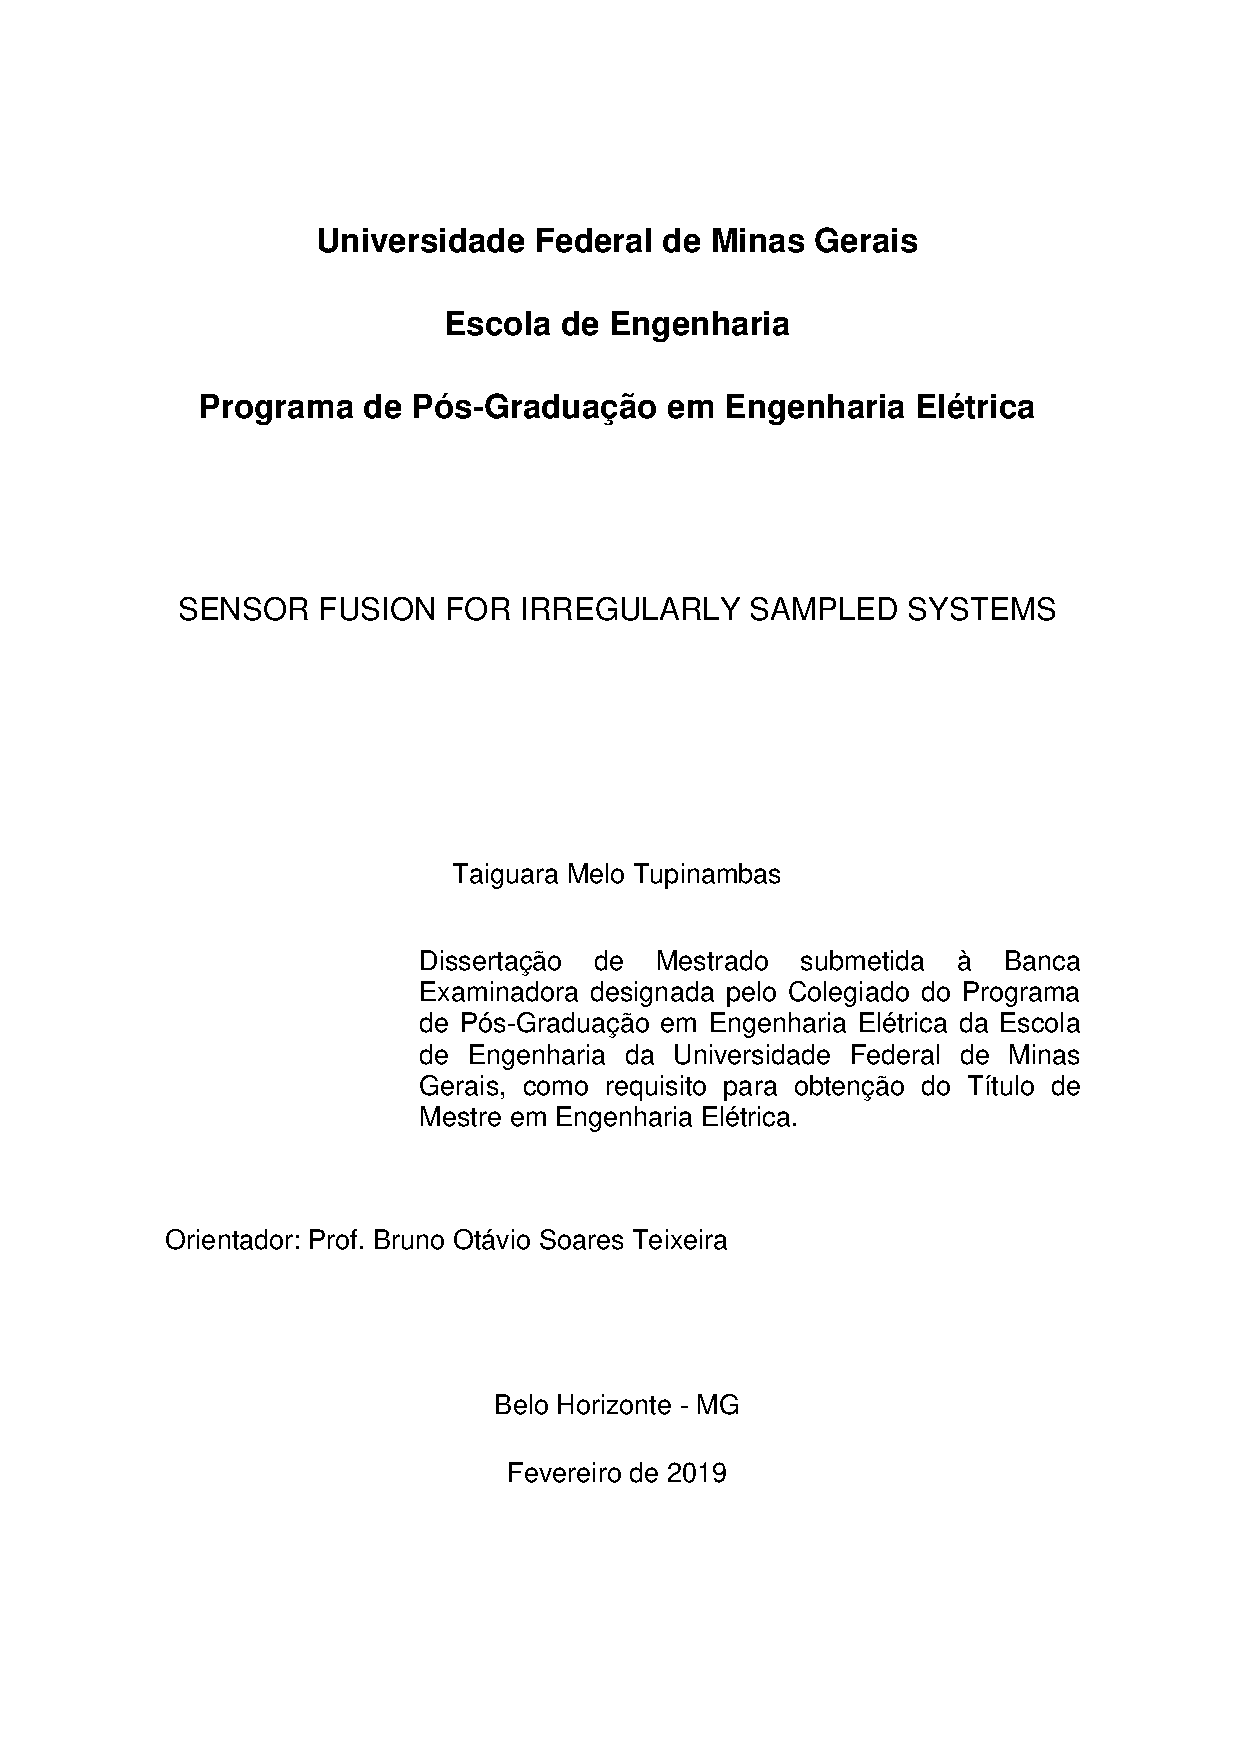
\includepdf[pages=-]{folha_rosto.pdf}
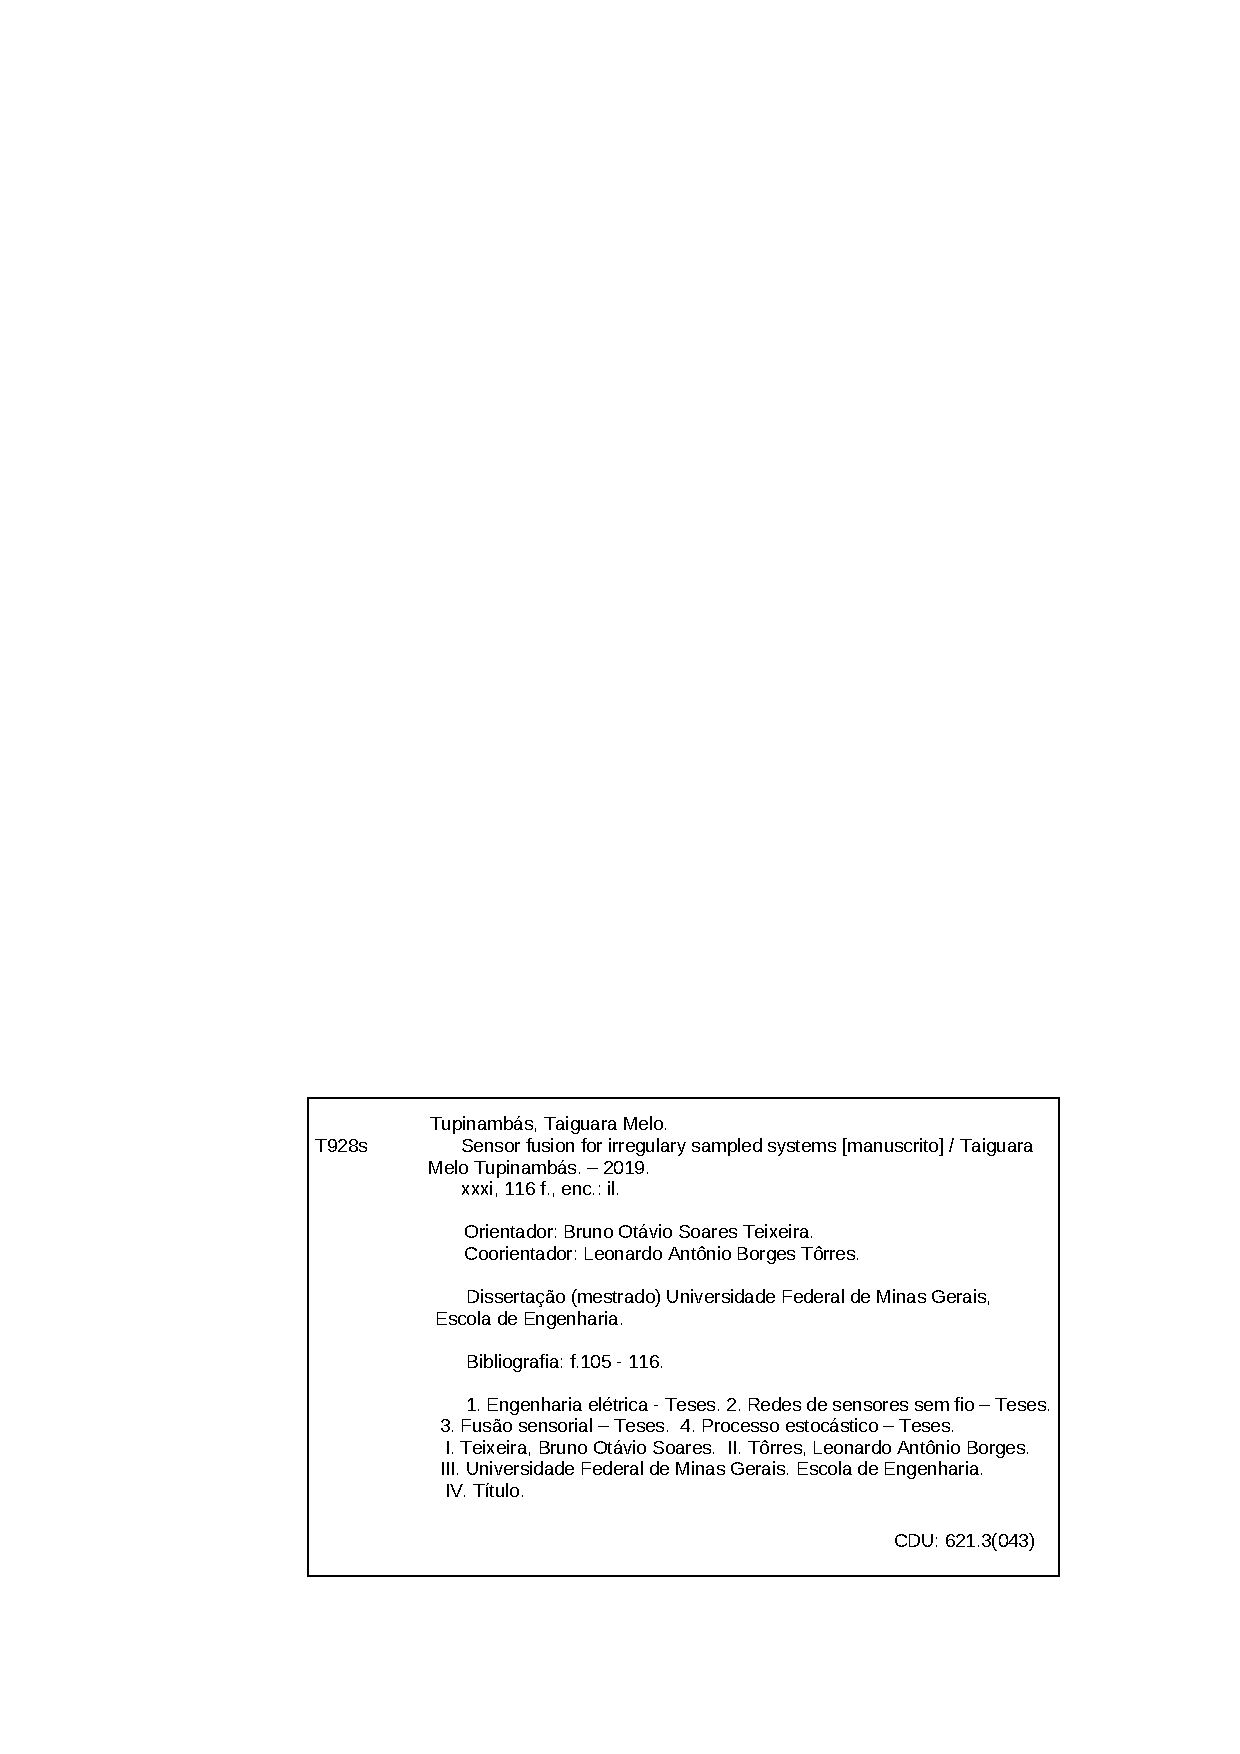
\includepdf[pages=-]{ficha_catalografica.pdf}
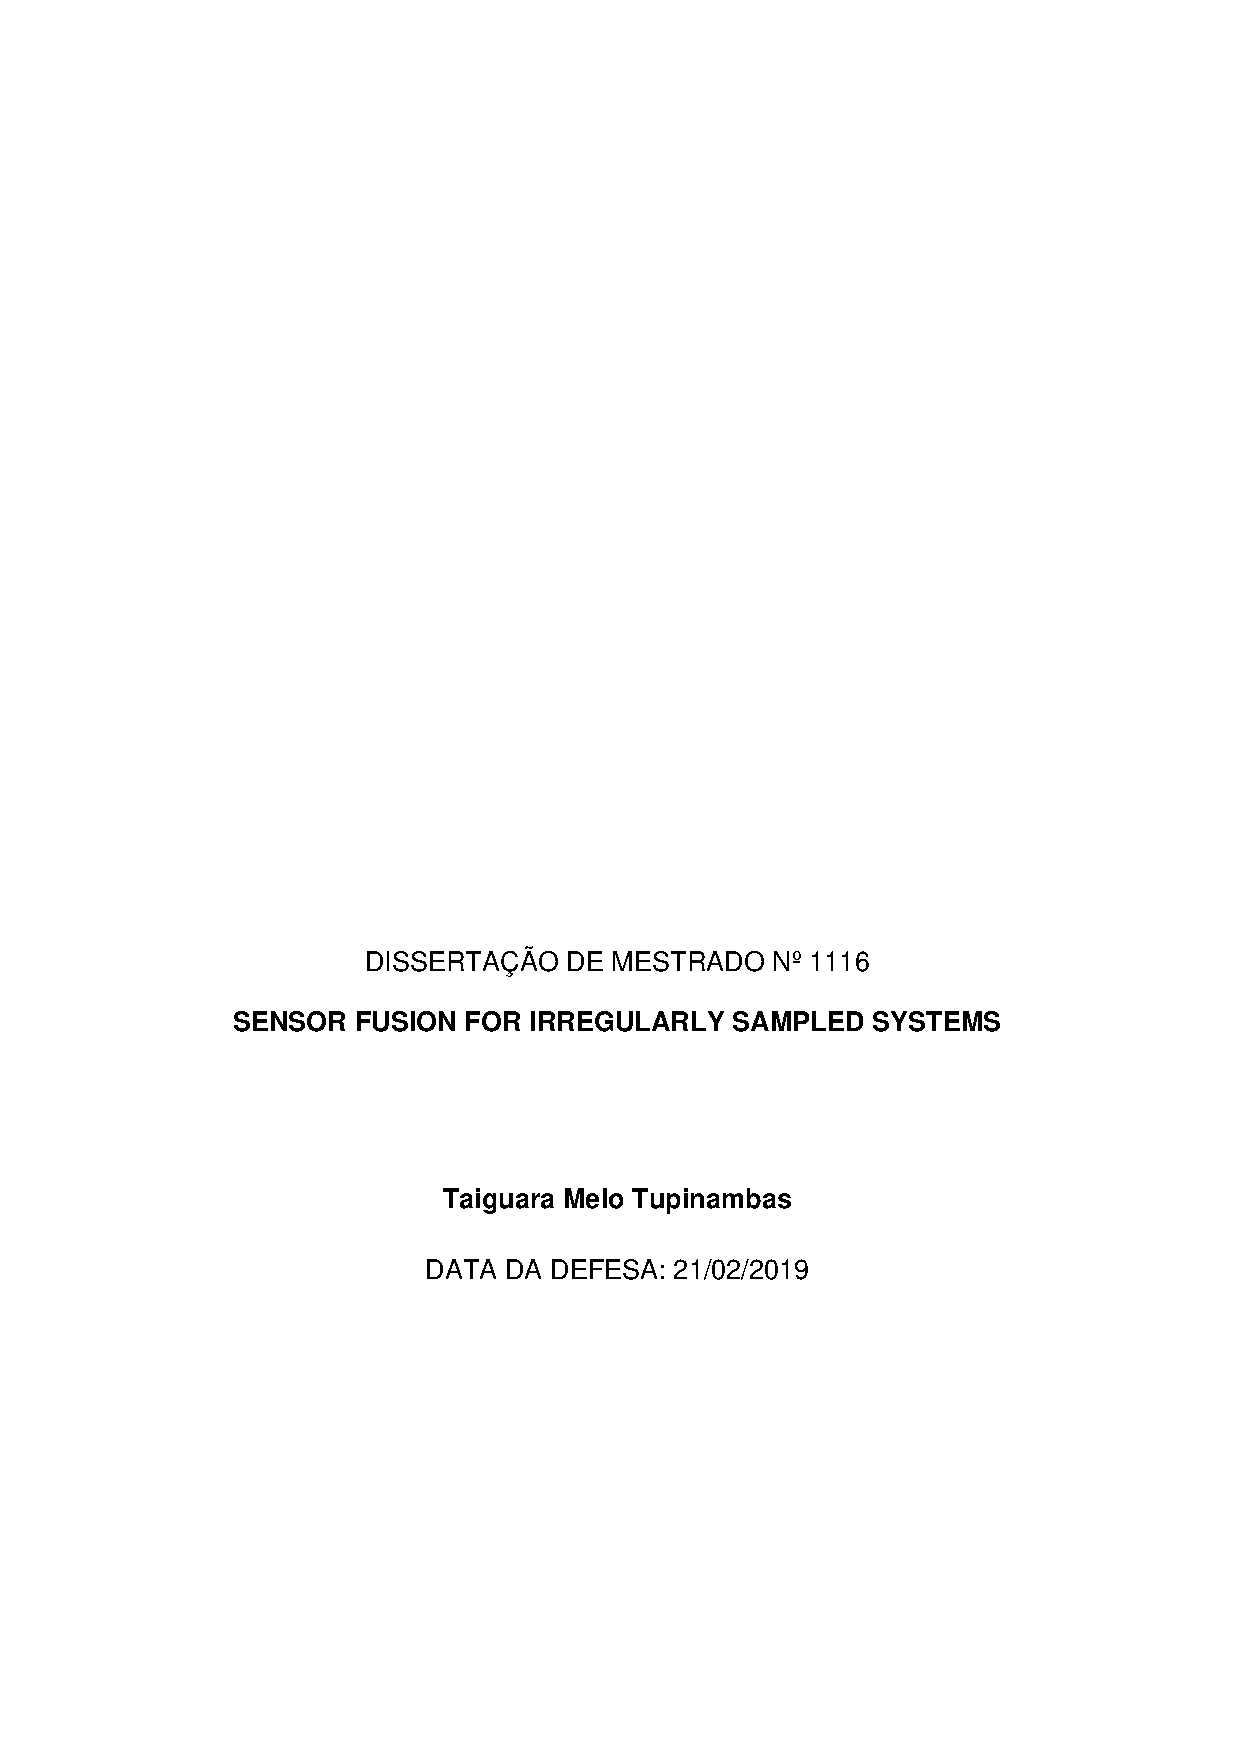
\includepdf[pages=-]{folha_numero.pdf}
%%CAPA
\begin{titlepage}

%Filia��o
%--------------------------------------------------------------------
\begin{figure}[!ht]
\begin{minipage}[b]{0.7\linewidth}
\begin{tiny}
Modeling, Analysis and Control of Nonlinear Systems Laboratory \\
Electronics Engineering Department \\
Federal University of Minas Gerais\\
Av. Ant�nio Carlos 6627, 31270-901 Belo Horizonte, MG Brasil\\
Phone: +55 3499-4866 - Fax: +55 3499-4850 %\\

\end{tiny}
\end{minipage}\hfill
\begin{minipage}[c]{0.3\linewidth}
\begin{flushright}
\vspace{-1.2cm}

\includegraphics[scale=1.37]{Imagens/mac.png}
\end{flushright}
\end{minipage}
\end{figure}
%--------------------------------------------------------------------

%T�tulo
%--------------------------------------------------------------------
\vspace{1.75cm}
\begin{center}
\thickhrulefill
\par\nobreak
\vspace*{10\p@}%
\hrule
\vspace*{10\p@}%
{\bf \Huge \bfseries  Sensor Fusion \\}
\vspace{0.25cm}
{\bf \Huge \bfseries  for Irregularly Sampled Systems}
\vspace*{10\p@}%
\hrule
\vspace*{40\p@}%
%--------------------------------------------------------------------

%Autor
%--------------------------------------------------------------------
{\large \bf Taiguara Melo Tupinamb�s}\\[0.5cm]
\end{center}
%--------------------------------------------------------------------


%Descri��o
%--------------------------------------------------------------------
\vspace{1.75cm}
\begin{flushright}
\begin{minipage}{0.7\linewidth}
Master Dissertation submitted to the Graduate Program in Electrical Engineering of the School of Engineering of the Federal University of Minas Gerais in partial fulfillment of the requirements for the Master's Degree in Electrical Engineering.\\
\end{minipage}
\end{flushright}
\vspace{1.6cm}


%--------------------------------------------------------------------

%Orienta��o
%--------------------------------------------------------------------
\begin{tabular}{ll}
  {\bf Advisors:} & Prof. Bruno Ot�vio Soares Teixeira, Dr.\\
    &                        Prof. Leonardo Ant�nio Borges T�rres, Dr.\\
\end{tabular}
\vspace{1.6cm}

%--------------------------------------------------------------------
%Cidade e Data
%--------------------------------------------------------------------
\centerline{Belo Horizonte, February, 2019}
%--------------------------------------------------------------------
\end{titlepage}

\clearpage
\thispagestyle{empty}
\cleardoublepage

%%--------------------------------------------------------------------
%
%%--------------------------------------------------------------------
%%Dedicat�ria
%Dedicuum cest laborae a quelquis personatum que ajudorat a facirelo.

%\clearpage
%\thispagestyle{empty}
%\cleardoublepage
%%--------------------------------------------------------------------
%
%
%%--------------------------------------------------------------------
%Agradecimentos
\chapter*{Agradecimentos}

Antes de tudo, sou grato � UFMG por ter me proporcionado toda uma estrutura de excel�ncia, para a realiza��o dos meus estudos. � atrav�s de institui��es p�blicas de ensino superior como ela que podemos evoluir como sociedade. Estendo meus agradecimentos ao PPGEE-UFMG e aos seus funcion�rios, professores e alunos que contribuiram para o desenvolvimento deste trabalho. E ao CNPq, pelo apoio financeiro durante grande parte do meu mestrado.

Agrade�o aos meus orientadores, Prof. Bruno Teixeira e Prof. Leonardo T�rres, por todo o ensinamento e pela forma contagiante com que compartilham suas experi�ncias. Serei eternamente grato por terem me acolhido de volta � Academia, ap�s longos anos.

Aos amigos do Laborat�rio de Modelagem, An�lise e Controle de Sistemas N�o-Lineares (MACSIN), pelo companheirismo e apoio. Aprender junto com voc�s foi incr�vel.

Tamb�m tenho muito a agradecer � equipe do Laborat�rio de Nanoespectroscopia (LabNS), � qual me juntei recentemente, e que tem renovado de forma constante a minha paix�o pela ci�ncia.

�s amigas e aos amigos do Bloco Pr�-Sal, por trazerem leveza e alegria aos meus dias, al�m de serem modelos exemplares que tenho para a vida. � turma de gradua��o da El�trica, em especial ao Igor Baratta, grande amigo e conselheiro. 

Termino esses agradecimentos, mencionando aqueles sem os quais nada faria sentido nem seria poss�vel. Aos meus pais, Marilu e Ubiratan, � minha irm� e ao meu cunhado, Moara e Matheus, agrade�o imensamente pela forma��o, pela confian�a, pelos conselhos e pelo amor incondicional. Voc�s me fazem muito feliz. Aos meus sobrinhos, Iara e Cau�, pelo carinho e pela inspira��o. � minha amada esposa Marina, meu porto seguro. Voc� me faz ser uma pessoa melhor todo dia. E �s minhas fam�lias Melo e Tupinamb�s, pelo amor e pelo incentivo constantes.
\\

\clearpage
\thispagestyle{empty}
\cleardoublepage
%%--------------------------------------------------------------------
%
%
%%--------------------------------------------------------------------
%Ep�grafe
\chapter*{Epigraph}

\vspace*{\fill}
\begin{flushright}
\epigraph{\itshape "Vamos colocar nas m�os do �ndio \\ os bot�es da inform�tica. \\ Vamos preparar com raio laser \\ uma grande feijoada.}{---Carlos Fernando, \textit{P�tria Amada}}
\vspace{3cm}
\end{flushright}

\clearpage
\thispagestyle{empty}
\cleardoublepage
%%--------------------------------------------------------------------


%%--------------------------------------------------------------------
%Sum�rio
\pagestyle{myheadings}
\begin{spacing}{1.5}
\tableofcontents
\end{spacing}
\thispagestyle{empty}
\cleardoublepage

%%
%%%--------------------------------------------------------------------
%Resumo
\begin{spacing}{1}
Lorem ipsum dolor sit amet, consectetur adipisicing elit, sed do eiusmod tempor incididunt ut labore et dolore magna aliqua. Ut enim ad minim veniam, quis nostrud exercitation ullamco laboris nisi ut aliquip ex ea commodo consequat. Duis aute irure dolor in reprehenderit in voluptate velit esse cillum dolore eu fugiat nulla pariatur. Excepteur sint occaecat cupidatat non proident, sunt in culpa qui officia deserunt mollit anim id est laborum.

Sed ut perspiciatis unde omnis iste natus error sit voluptatem accusantium doloremque laudantium, totam rem aperiam, eaque ipsa quae ab illo inventore veritatis et quasi architecto beatae vitae dicta sunt explicabo. Nemo enim ipsam voluptatem quia voluptas sit aspernatur aut odit aut fugit, sed quia consequuntur magni dolores eos qui ratione voluptatem sequi nesciunt. Neque porro quisquam est, qui dolorem ipsum quia dolor sit amet, consectetur, adipisci velit, sed quia non numquam eius modi tempora incidunt ut labore et dolore magnam aliquam quaerat voluptatem. Ut enim ad minima veniam, quis nostrum exercitationem ullam corporis suscipit laboriosam, nisi ut aliquid ex ea commodi consequatur? Quis autem vel eum iure reprehenderit qui in ea voluptate velit esse quam nihil molestiae consequatur, vel illum qui dolorem eum fugiat quo voluptas nulla pariatur?

\keywords{Vis�o Computacional, Redes, Sabotagens}

\clearpage
\thispagestyle{empty}
\cleardoublepage
%%--------------------------------------------------------------------
%
%%--------------------------------------------------------------------
%Abstract
\chapter*{Abstract}
\addcontentsline{toc}{chapter}{Abstract}

\vspace{-2cm} 
The use of multiple sensors to improve data quality has grown continuously over the last few decades. With the never-ending advances in technology of microprocessors and communication devices, sensor networks will continue to increase in both size and complexity. The most popular applications for fusing data from various sources are related to estimating the states of a dynamic system. For that, two noisy sources of information are needed: a process model that describes how the states evolve in time; and an observation model, whose data are usually obtained from sensors. Since most sensors are digital, signals must be sampled in order to be processed, leading to sampled-data systems. Classical state estimators in these cases, like the well-known Kalman filter, implicitly consider regularly sampled signals with constant time intervals between samples, such that continuous-time systems can be time discretized into time-invariant representations in most cases. However, because of the widespread use of complex sensor networks without explicit time synchronization, many applications cannot rely on data being transmitted regularly. There are adaptations to state estimation techniques that handle most of the irregularities, provided that timestamps are part of measurement packets and that the increase in computational processing time is acceptable. If timestamps cannot be used in the estimation process, one can either invest in synchronization or accept the assimilation of information at incorrect time instants. The effects in estimation performance of the latter approach has not yet been extensively studied. In this work we investigate how performance is deteriorated by neglecting measurements timestamps in state estimation algorithms. We consider the Poisson process as a model to generate the irregular time instants sequences, and we assess state estimation results for linear and nonlinear systems simulated with aperiodic sampling, using the Kalman filter for the former and its adapted unscented version for the latter. Algorithms are designed to use timestamps or to neglect them in the estimation process, and their results over multiple runs are compared for different simulation scenarios. Finally, we identify and discuss relations between different sets of parameters, such as signal-to-noise ratios and average sampling frequencies, and the degradation in performance.
\\ \\
\textbf{Keywords:} Sensor Fusion; Irregular Sampling; State Estimation; Sampled-data Systems; Time Synchronization; Time-Stamp.

\clearpage
\thispagestyle{empty}
\cleardoublepage
\end{spacing}
%%%--------------------------------------------------------------------
%%
%%%--------------------------------------------------------------------
%%%Lista de figuras
\begin{sloppypar}
\listoffigures
\end{sloppypar}
\addcontentsline{toc}{chapter}{List of Figures}
\clearpage
\thispagestyle{empty}
\cleardoublepage
%%
%%%--------------------------------------------------------------------
%%%Lista de Tabelas

\listoftables
\addcontentsline{toc}{chapter}{List of Tables}
\clearpage
\thispagestyle{empty}
\cleardoublepage

%
%%%--------------------------------------------------------------------
%%%S�mbolos
%%%--------------------------------------------------------------------
\chapter*{List of Symbols and Acronyms}
\addcontentsline{toc}{chapter}{List of Symbols and Acronyms}
%\vspace{-2.0cm}
\section*{Symbols}

\setlength{\LTleft}{10pt}

\subsection*{Chapter 1}

\begin{longtable}{ll}
	$\mathbb{N}^+$			& positive integers; \\
	$\mathbb{R}$			& real numbers; \\
	$\mathbb{R}^n$			& $\mathbb{R}^{nx1}$ $n$-dimensional Euclidean space; \\
	
	$\forall$				& for all; \\
	$\in$					& belongs to; \\
	$>$						& greater than; \\
	$<$						& less than; \\
	$\geq$					& greater than or equal to; \\
	$\leq$					& less than or equal to; \\
	$\triangleq$			& equals by definition; \\	
	$\approx$				& approximately equal to; \\
	$\sim$					& is distributed as; \\
	
	$\mathcal{N}$			& Gaussian distribution; \\
	$\mathcal{E}$			& Exponential distribution; \\
	$x_i$					& $i$th entry of x; \\	
	
	$f$						& process model; \\
	$g$						& observation model; \\
	$t$						& continuous-time index; \\
	$k$						& discrete-time index of measurements; \\
	$i$						& discrete-time index of input; \\
	$t_k$					& continuous-time sampled instants; \\
	$T$						& input sampling interval; \\
	$x(t)$					& state vector; \\
	$x(t_k)$				& state vector at continuous-time sampled instants; \\
	$u(t)$					& input vector; \\
	$u(iT)$					& input vector at continuous-time sampled at time $t = iT$; \\						
	$w(t)$					& process noise vector; \\
	$y_{t_k}$            	& output vector at continuous-time sampled instants;\\
	$\delta_{k}$			& measurements time-delay; \\
	$v(t_k)$				& measurement noise vector; \\
	$h_k$					& time intervals between two continuous-time sampled instants; \\
	$\lambda$ 				& parameter of the exponential distribution; \\
	$\lambda_h$				& parameter of the exponentially distributed random variable $h_k$; \\
	$\lambda_{\delta_{k}}$	& parameter of the exponentially distributed random variable $\delta_{k}$; \\
	$N$						& amount of identical sensors in the sampling model; \\
	$L$						& sampling period of the identical sensors in the sampling model; \\
	$P$						& covariance matrix; \\
	$\alpha$				& relation between output (expected) and input sampling time intervals . \\
\end{longtable}

\subsection*{Chapter 2}

\begin{longtable}{ll}
	$\mathcal{N}$			& Gaussian distribution; \\
	$\mathbb{P}$			& power set; \\
	
	$\mu$ 					& mean of a random variable; \\
	$\sigma$ 				& standard deviation of a random variable;\\
	
	$n$						& number of homogeneous sensors; \\
	$E$						& evidence; \\ 
	$H$						& hypothesis; \\
	$R_r$					& $r^{th}$ fuzzy rule; \\
	$x_k$					& $k^{th}$ input fuzzy variable; \\
	$A_i$					& $i^{th}$ antecedent linguistic value; \\
	$y$						& output variable; \\
	$C_j$					& $j^{th}$ consequent class; \\
	$A$						& fuzzy set; \\
	$U$						& universe of discourse; \\
	$B$						& subset of features; \\
	$B_*(X)$				& \textit{B-lower} approximation of $X$; \\
	$B^*(X)$				& \textit{B-upper} approximation of $X$; \\
	$BN_B(X)$				& \textit{B-boundary} region of $X$; \\
	
	$\rho(x)$				& probability distribution of $x$; \\
	$\rho(A|B)$				& conditional probability distribution of $A$ given $B$; \\
	$\pi_x(u)$				& possibility distribution of $x$ associated with $u$; \\
	$\mu_A(x)$				& membership function of $x$ of a fuzzy se $A$; \\
	
	
	$\subseteq$				& is a subset of; \\
	$\cap$					& set intersection; \\
	$\emptyset$				& empty set; \\
	
\end{longtable}


\subsection*{Chapter 3}

\begin{longtable}{ll}
	$\mathbb{N}$			& natural numbers; \\
	$\mathbb{R}$			& real numbers; \\
	$\mathbb{R}^n$			& $\mathbb{R}^{nx1}$ $n$-dimensional Euclidean space; \\
	
	$Ber(p)$				& Bernoulli distribution; \\
	$\mathcal{N}$			& Gaussian distribution; \\
	$\Gamma$				& gamma distribution; \\
	
	$\forall$				& for all; \\
	$>$						& greater than; \\
	$\geq$					& greater than or equal to; \\
	$\sim$					& is distributed as; \\
	$\pm$					& plus or minus; \\
	
	$y_{t}$, $y{k}$           	& output vector at continuous-time sampled instants;\\
	$z(t)$						& measurement output; \\
	$H(k)$, $L(k)$, $C$, $D$ 	& matrices of the observation model; \\
	$v(t)$, $v(k)$				& measurement noise vector; \\
	$t_i$ 					& continuous-time sampled index; \\
	$k$						& discrete-time index of measurements;  \\
	$T$						& expected time interval; \\
	$d(k)$					& observation sampling time delays; \\
	$l$						& amount of different known delays; \\
	$\xi(t)$				& random variable that models packet dropout; \\
	$\gamma(t)$				& random variable that models uncertain observation; \\
	$C_i(t)$				& real time approximation from the $i^{th}$ computer clock; \\
	$a_i$					& $i^{th}$ clock drift; \\
	$b_i$					& $i^{th}$ clock offset; \\
	$a_{ij}$				& relative drift between $i^{th}$ and $j^{th}$ node; \\
	$b_{ij}$				& relative offset between $i^{th}$ and $j^{th}$ node; \\

	$\Delta$				& measured value interval between observations; \\
	$\delta_k$				& random time interval; \\
	
	$p(k)$					& Bernoulli distribution parameter; \\
	$\epsilon_k$			& deviation from expected time instants; \\
	$\sigma$				& standard deviation; \\
	$\kappa$				& shape parameter; \\
	$\theta$				& scale parameter; \\
	
	$\mu s$					& micro seconds; \\
	$E.E$					& energy efficiency; \\
	$Comp.$					& complexity; \\

\end{longtable}


\subsection*{Chapter 4}

\begin{longtable}{ll}
%	$\mathbb{N}$			& natural numbers; \\
%	$\mathbb{R}$			& real numbers; \\
%	$\mathbb{R}^n$			& $\mathbb{R}^{nx1}$ $n$-dimensional Euclidean space; \\
	
%	$\mathcal{N}$			& Gaussian distribution; \\
	
	$\triangleq$			& equals by definition; \\	
%	$>$						& greater than; \\
%	$\geq$					& greater than or equal to; \\
%	$\sim$					& is distributed as; \\
%	$\pm$					& plus or minus; \\
	$\operatorname{arg}  
	\underset{x}
	{\operatorname{max}} 
					f(x)$	& argument $x$ that maximizes function $f(x)$; \\ 
					
	$\rho(x|y)$				& conditional probability density function of $X$ given $Y$; \\
	$x_k$						& state vector; \\
	$\hat{x_k}$				& estimated state vector; \\
	$y$						& observation vector; \\
	
%
%	$\sigma$				& standard deviation; \\
%	$\kappa$				& shape parameter; \\
%	$\theta$				& scale parameter; \\
	
	
\end{longtable}



\subsection*{Chapter 5}

\newpage
\section*{Acronyms}
\begin{longtable}{ll}
	CDF			& Cumulative Distribution Function; \\
	CU			& Covariance Union; \\
	DAI			& Data In; \\
	DAO			& Data Out; \\
	DEI			& Decision In; \\
	DEO 		& Decision Out; \\
	DMTS		& Delay Measurement Time Synchronization; \\
	DSET 		& Dempster-Shafer Evidence Theory; \\		
	EKF			& Extended Kalman Filter; \\
	FEI			& Feature In; \\
	FEO			& Feature Out; \\
	FIS			& Fuzzy Inference System; \\
	FISST		& Finite-Set Statistics; \\
	FTSP		& Flooding Time Synchronization Protocol; \\
	GPS			& Global Positioning System; \\
	HMM			& Hidden Markov Model; \\
	KF 			& Kalman Filter; \\
	UKF			& Unscented Kalman Filter; \\
	LEETS		& Lightweight and Energy Efficient Time Synchronization; \\
	LTS			& Lightweight Tree-based Synchronization; \\
	LS			& Least Squares; \\
	MAP			& Maximum A Posteriori; \\
	ML			& Maximum Likelihood; \\
	MMSE		& Minimum Mean Square Error; \\
	MOP 		& Measures Of Performance; \\
	NEES		& Normalized Estimation Error Squared; \\
	NIS			& Normalized Innovation Squared; \\
	NMR 		& Nuclear Magnetic Resonance; \\
	NTP			& Network Time Protocol; \\
	NUS 		& Non-Uniform Sampling; \\ 
	OOSM 		& Out-Of-Sequence Measurement; \\
	PDF         & Probability Density Function; \\
	PDAF		& Probabilistic Data Association Filter; \\
	PF 			& Particle Filter; \\
	RBS			& Reference Broadcast Synchronization; \\
	RMSE		& Root Mean Square Error; \\
	RTPF		& Real-Time Particle Filter; \\
	RV			& Random Variable; \\
	SOD			& Send-On-Delta; \\
	SNR			& Signal-to-Noise Ratio; \\
	TDS			& Time-Delay System; \\
	TDP			& Time-Diffusion Protocol; \\
	TPSN		& Timing-sync Protocol for Sensor Networks; \\
	TSST		& Time Synchronization based on Spanning Tree; \\
	TTF 		& Track-to-Track Fusion; \\
	UKF			& Unscented Kalman Filter; \\
	WSN			& Wireless Sensor Networks; \\
	ZOH			& Zero-Order Holder; \\
\end{longtable}


\clearpage
\thispagestyle{empty}
\cleardoublepage
\normalsize
%%%%--------------------------------------------------------------------
%%%
%%%%Abreviaturas
%%%%%--------------------------------------------------------------------
%\chapter*{List of Acronyms}
\addcontentsline{toc}{chapter}{Lista de Acr�nimos}

\vspace{-2.0cm}

\begin{tabular}{ll}
CDF			& Cumulative Distribution Function \\
DAI			& Data In \\
DAO			& Data Out \\
DEI			& Decision In \\
DEO 		& Decision Out \\
DSET 		& Dempster-Shafer Evidence Theory \\		
EKF			& Extended Kalman Filter \\
FEI			& Feature In \\
FEO			& Feature Out \\
KF 			& Kalman Filter \\
MOP 		& Measures Of Performance \\
NMR 		& Nuclear Magnetic Resonance \\
NUS 		& Non-Uniform Sampling \\ 
OOSM 		& Out-Of-Sequence Measurements \\
PDF         & Probability Distribution Function \\
PF 			& Particle Filter \\
SOD			& Send-On-Delta \\
TDS			& Time-Delay System \\
UKF			& Unscented Kalman Filter \\
\end{tabular}

%\clearpage \thispagestyle{empty}
%\cleardoublepage

%--------------------------------------------------------------------


%Come�ando os cap�tulos
%--------------------------------------------------------------------
\clearpage
\pagestyle{myheadings}
\pagenumbering{arabic}
%--------------------------------------------------------------------

%--------------------------------------------------------------------
%Defini��o de cabe�alhos
\pagestyle{fancy}
\renewcommand{\chaptermark}[1]{\markboth{\thechapter\ #1}{}}
\renewcommand{\sectionmark}[1]{\markright{\thesection\ #1}{}}
\fancyhf{}
\fancyhead[LE,RO]{\thepage}
\fancyhead[LO]{\rightmark}
\fancyhead[RE]{\leftmark}
\renewcommand{\headrulewidth}{0.5pt}
\renewcommand{\footrulewidth}{0.0pt}
\addtolength{\headheight}{2.5pt}                % 2.5pt
\fancypagestyle{plain}{
     \fancyhead{}
     \renewcommand{\headrulewidth}{0pt}
     }
 
%--------------------------------------------------------------------
%Cap�tulo 1 - Introdu��o
\chapter{Introduction}
\label{cap1} \vspace{-1cm}

%
%\begin{flushright}
%\begin{minipage}{0.7\linewidth}
%\emph{``Em verdade, em verdade vos digo: quem ouve a minha palavra e
%cr� naquele que me enviou tem a vida eterna, n�o entra em ju�zo, mas
%passou da morte para a vida.''}
%\end{minipage}
%\end{flushright}
%
%\begin{flushright}
%{Jo 5:24}
%\end{flushright}

\section{Motivation}\label{motivation}

In nature it is possible to observe data fusion in a variety of phenomena. Animals combine signals from different senses, such as sight, hearing, smell, taste and touch, to recognize the surroundings. Plants have analogous mechanisms, which are used to modulate water consumption, to change the color of its leaves or to bend its structure towards the light, for instance. Throughout history, the sensory systems in living beings have evolved to assimilate multiple information coming from numerous sources in a highly complex and efficient way, in order to have a better perception of the environment. 

Nowadays information fusion is studied in many fields of science, as a way of exploiting data from multiple sources to achieve better outcomes in comparison to those obtained if any of the sources were used separately \citep{Dasarathy2001}. Other terms have been used to denote the synthesis of information in technical literature, for instance, data fusion, sensor fusion, combination of evidence and synthesis of observations \citep{Goodman1997}. To avoid confusion, the terminology used by \citep{Elmenreich2002} will be adopted, whereby information fusion is understood as the overall term and sensor fusion is used in cases for which the sources of information are sensors. 

Some research fields have been increasingly exploiting the advantages of sensor fusion techniques, such as robotics, military, biometrics and image processing. The main benefits expected are related to accuracy, due to the use of redundant or complimentary data; to dimensionality, that is additional information being created by a group of data; and to robustness against failures and interference. Consequently much effort has been put into the development and investigation of data fusion techniques. The work of \citep{Khaleghi2013} presents an extensive review of different approaches available, categorizing them by the way sensor data imperfection is represented, namely, probabilistic fusion, evidential belief reasoning, fuzzy reasoning, possibilistic fusion, rough set-based fusion, random set-based fusion and hybrid fusion. 

Data fusion techniques based on probability theory are the earliest available and perhaps the most popular until now. They are concerned with estimating the probability distribution functions (PDF) of the system states by means of the Bayesian approach. If the system is linear and Gaussian, then the Kalman filter (KF) guarantees optimal estimation. For nonlinear processes, KF generalizations were proposed, such as the extended Kalman filter (EKF) or the unscented Kalman filter (UKF) \citep{Julier2004}. On the other hand, particle filters (PF) can be used to deal with both nonlinearities in the dynamics and non-Gaussian distributions \citep{Arulampalam2002}.

The most common class of systems studied in state estimation is the class of sampled-data systems, due to the wide use of digital devices. Although often described by continuous time differential equations, they can be modeled using discrete state equations, using approximation techniques \citep{Phillips1995}. Usually the sampling period of such systems are constant and known. In other words, the sensors are considered to transmit data at regular intervals. However, for many applications, such assumption is not valid. The use of several redundant sensors, for example, with different sampling rates or unsynchronized with one another, leads to data being received at irregular instants. Additionally, when data from multiple sensors are transmitted through several subsystems in a network, there might be loss of packets and delays \citep{Schenato2007} or even multiple information arriving simultaneously \citep{Moayedi2011}. In networked control systems, event-triggered sampling schemes have been proposed to optimize the access to communication channels \citep{Hu2017}, which will also generate time-varying sampling intervals. Nowadays, because of the ever-growing scientific advances, the technology of microprocessors, sensors and communication has become increasingly accessible, which continues to ensure that multiple sensor networks are more and more common.

Thus, despite improving accuracy and robustness of the estimation process, the fusion of data from multiple sensors might introduce challenges to the state estimation algorithms, due to sampling irregularities. Depending on how they take place, modifications to the KF and its generalizations can be carried out to tackle these abnormalities. In the work of \citep{Fatehi2017}, a fusion KF is proposed to estimate the states of a system with multi-rate measurements, whereby one of them is fast, regular and delay-free and the other is slow, irregular and randomly delayed. One application of such system is for industrial process control, where there is online instrumentation characterized by the former and data from laboratory analysis, which are much more accurate. For a more general case, when the random delays are unknown, the work of  \citep{Gopalakrishnan2010} presents a critical analysis of the available methods for data fusion. They are separated into two categories: those that incorporate the delayed measurements upon arrival, and methods that rely in state augmentation, in order to assimilate the delayed information between estimation steps. 

In general the proposed methods and their performance will depend on the characteristics of the sampling irregularities and how they are modeled. Time delays can be multiples of a base sampling period, for instance. In those cases, delays can happen at single or multiple lags \citep{Penarrocha2012}, can lead to out-of-sequence measurements \citep{Anxi2005, Westenberger2013} or there can also be data dropout \citep{Zhu2013}. Nevertheless, the system can be described by a time-invariant discrete state equation, but with a particular representation of the measurement model. When the instants take place after random time intervals, the discrete-state representation leads to a time-varying system, since the sampling period changes over time. Some researches treat the variable measurement instants as stochastic processes \citep{Micheli2002} or as a periodic sampling interval subject to noisy perturbations \citep{Shen2016}. Generally, the instant is considered to be known and the methods assimilate such information in the algorithm.

To the best of the author's knowledge, no method was proposed so far to take the irregularity into account and improve the estimation efficiency, for the cases in which the random time instant the signal was measured and its statistics are not known or not reliable. If the sampling irregularity is caused due to the lack of sensor synchronization in the network, several algorithms can ensure a common timescale \citep{Sivrikaya2004}, at the expense of additional investments or energy use. Another approach, believed to be largely used on practice, is to disregard the irregularities, assimilating the measurements as soon as possible \citep{Kwok2004, Huck2011}. In this case, additional noises are tuned in the estimation process, but it might be irrelevant to the overall performance.

Knowing to what extent the estimation accuracy is deteriorated by ignoring the additional uncertainty caused by the sampling irregularity is important to decide whether or not to invest in synchronization. In addition, the investment in more sensors to the network in order to improve accuracy might not pay off, if it increases the occurrence of irregularities. However there are no detailed studies on the behavior of the degradation in accuracy due to neglecting the irregularity in the sampling process. Therefore, this work assesses the differences in state estimation performance for systems with random sampling intervals with and without timestamp for different scenarios. The purpose is to shed some light on the trade-off for investments in sensor networks and synchronization.

\section{Problem Formulation}\label{problem-formulation} 

Consider the stochastic nonlinear sampled system
	
\begin{equation}\label{eq:processo}
\dot{x}(t)=f(x(t), u(t), w(t), t),
\end{equation}
\begin{equation}\label{eq:obs}
y(t_k)=g(x(t_k- \delta_{k}) ,v(t_k), t_k),
\end{equation}
\\
\noindent
where 	$f\!\!: \mathbb{R}^n \times \mathbb{R}^p \times \mathbb{R}^q \times \mathbb{R^+} \rightarrow \mathbb{R}^n $ and $g\!\!: \mathbb{R}^n \times \mathbb{R}^r \times \mathbb{R^+} \rightarrow \mathbb{R}^m $ are, respectively, the process and observation models, considered as known. We assume that for all $k \geq 1$, the observations $y(t_k) \in \mathbb{R}^m$ and the first two moments of the random variables $x_0$, $v(t_k)$ and $w(t)$ are known, where $x_0 \in \mathbb{R}^n$ is the initial state vector, $v(t_k) \in \mathbb{R}^r$ is the observation noise and $w(t_k) \in \mathbb{R}^q$ is the process noise. Observations are taken at random time instants $t_k$ and are considered to be sorted ($t_{k+1}>t_k,\forall k \in \mathbb{N^+}$) and defined by the time intervals $h_0 \triangleq t_1$, $h_k \triangleq t_k-t_{k-1}, \ \forall k \geq 1$. In this work, we assume that the observation time instants $t_k$ are given by a Poisson random process. That is, the time intervals $h_k$ are independent and identically distributed (i.i.d.) exponential random variables with a known parameter $\lambda_{h}$, that is $h_k \sim \mathcal{E} (\lambda_{h})$,  where $\mathcal{E} (\lambda)$ defines an exponential PDF, with parameter $\lambda$, which is also its expected value. An example of time intervals produced by such a random process is illustrated in Figure \ref{fig:amost}.


\begin{figure}[h]
	\centering
	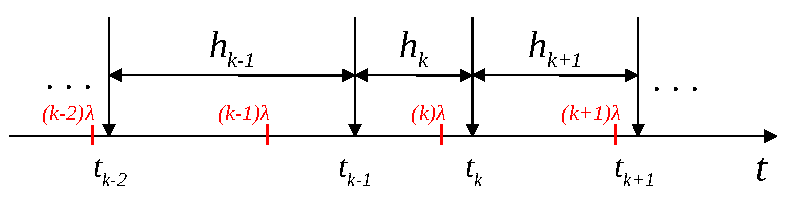
\includegraphics[width=0.8\textwidth]{Imagens/processo_amost.pdf}
	%\setlength{\belowcaptionskip}{-12pt}
	\caption[Irregular sampling process modeled by a Poisson random process]{Irregular sampling process modeled by a Poisson random process. Regularly spaced time intervals $\lambda$ are shown in red. An example of time instants $t_k$ realization is also shown, with the respective random time intervals $h_k$. The expected value of time interval is given by $E(h_k)=\lambda$.}
	\label{fig:amost}
\end{figure}

This sampling model characterizes a common application for an event-based sampling scheme or for a networked control system with unsynchronized sensors. \citep{Micheli2002}, for instance, considers a set of $N$ identical sensors measuring the state variables of a physical process every $L$ seconds. They prove that, if the sensors are independent and unsynchronized and $N$ is big enough, the waiting time between the realization of two consecutive measurements can be approximated by an exponential random variable $\mathcal{E} (\lambda)$, where the parameter is given by $\lambda = N/L$.

Arrival times to the estimator may be delayed during transmission by a random time amount $\delta_{k}$, also given by exponential random variables, with parameter $\lambda_{\delta_{k}}$, according to Figure~\ref{fig:delay}. Out-of-sequence measurements (OOSM) are not considered in this work. We assume that, in case a delayed measurement is to arrive later than future measurements, it gets lost in transmission.


\begin{figure}[h]
	\centering
	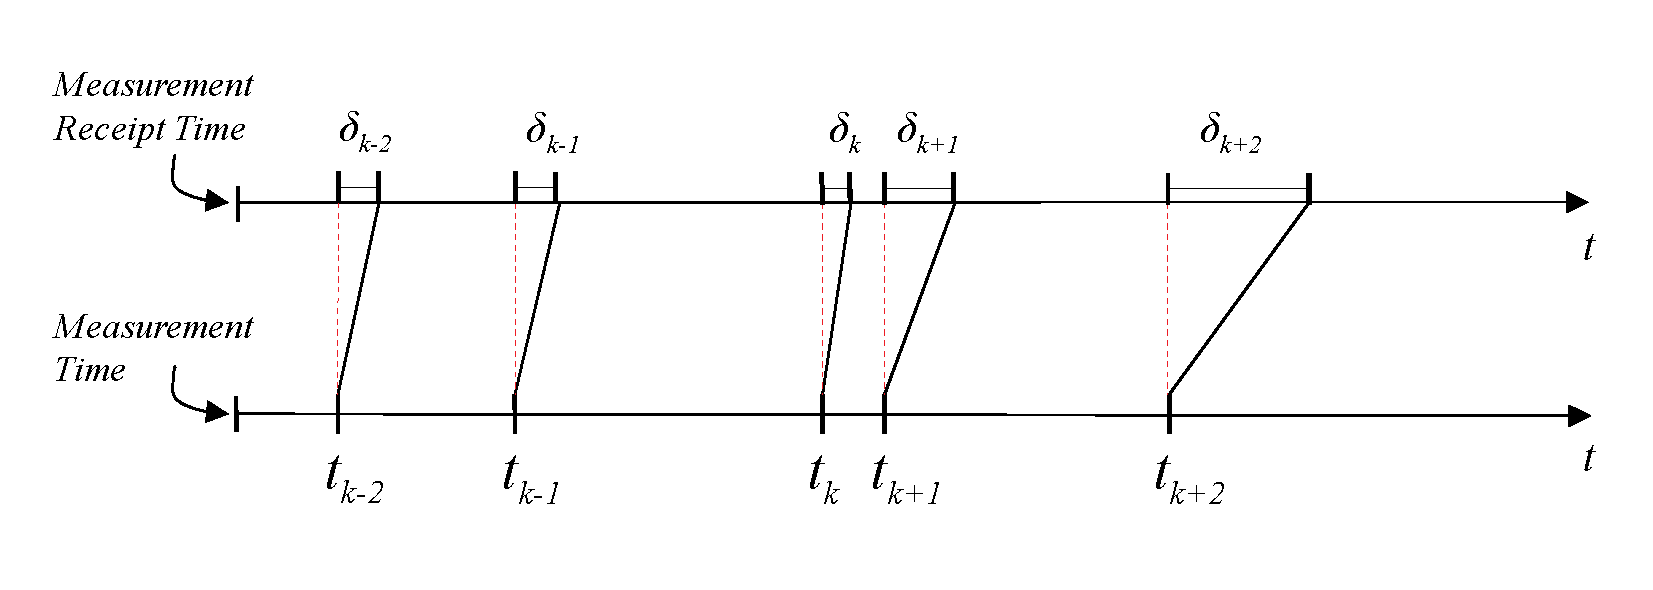
\includegraphics[width=1\textwidth]{Imagens/scheme-timedelay.pdf}
	%\setlength{\belowcaptionskip}{-12pt}
	\caption[Randomly delayed measurements, modeled as exponential random variables]{Randomly delayed measurements, modeled as exponential random variables. Random measurement times $t_k$ are received by the estimator after a random delay $\delta_{k}$}
	\label{fig:delay}
\end{figure}


Input data $u(t)$ are available at regularly spaced intervals $T$, that is $u(iT) \in \mathbb{R}^p$, $\forall i \geq 1$ are known.  $w(t) \in \mathbb{R}^q$ is process noise.

%\duvida{Como tratar a quest�o do filtro cont�nuo para as entradas u(t)}/

When time-stamp information is available, data assimilation can be performed at the correct measurement instants $t_k$. When they are not, the assimilation moment is considered to be the random receipt time instant or the next estimation moment, when there are no transmission time delays. 

We wish to estimate the state vector $x(t)$ and its covariance recursively, at regularly spaced time intervals $T$, given their initial values ($x_0$, $P_0$), the process model (\ref{eq:processo}), the input or control signals, $u(t): t \leq kT$, and the set of past observations, $y(t_k): t_k - \delta_{k} \leq kT$. The knowledge of the time intervals $h_{k-1}: t_k - \delta_{k} \leq kT$ is also taken into consideration when time-stamp information is available. We assume that the average time interval of observations $\lambda_{h}$ is greater than or equal to $T$ by a factor $\alpha\geq1$, i.e. $\lambda_{h}=\alpha T$.






\section{Objectives}\label{objectives}

%1 frase para o objetivo geral
%Objetivos espec�ficos

\section{Text Outline}\label{text-outline}
%
This text is organized in six chapters, including this one. Chapter~\ref{cap1} presents an introduction to the object of study, with an overview of the motivations and historical perspective of the theme, objectives and problem formulation.

Chapter~\ref{cap2} presents a review of the sensor fusion field of science, addressing not only the definitions and taxonomy, but also the advantages of combining information from multiple sources. From the four categorization models of the data fusion problem, the one based on data challenges is further explored. We then introduce and discuss the methods proposed in literature that handles imperfect data. 

Chapter~\ref{cap3} discusses the data-related challenges that arise for sampled-data systems, regarding sampling irregularities. Diagrams are built to organize the types, effects and causes of irregularities. We describe the necessary modifications to state estimation observation models, in order to handle such abnormalities in sampling schemes. In order to perform effective state estimation in the presence of sampling irregularities, methods depend on the knowledge of the exact time measurements were taken. Therefore, we explore time synchronization methods suited for sensor networks.

After the literature review, we focus on the probabilistic sensor fusion approach to sampled-data systems with sampling irregularities without time-stamp. The study of the impact of neglecting time-stamp information is performed.

Chapter~\ref{cap4} describes the methods used for simulation, considering the adaptations for the scenarios with and without time-stamp. We describe the filtering algorithm and the assumptions used for each scenario. Furthermore, we define the performance metrics used for the results assessment.

In Chapter~\ref{cap5} we present results from the simulation of two systems: an arbitrary linear system and a unicycle position estimation system. Signal parameters are varied to assess the impact in performance of both considering and not considering time-stamp in estimation algorithms. Performances are evaluated using estimated state errors and estimation consistency. 

Finally, we conclude the study in Chapter~\ref{cap6}, highlighting the study limitations and suggestions of future work, apart from evaluating if the proposed objectives were achieved.

\clearpage

%
%\subsubsection{Problema 1: In}\label{sec:entrada_regular}
%
%\textit{As entradas $u(t)$ s�o medidas em intervalos regularmente espa�ados $T$, i.e. $u(iT) \in \mathbb{R}^p$, $\forall i \geq 1$ s�o conhecidas. $w(t) \in \mathbb{R}^q$ � o ru�do de processo. 
%}
%
%\subsubsection{Problema 2: Irregular input sampling}\label{sec:entrada_irregular}
%
%\textit{Medi��es feitas em instantes de tempo aleat�rios $t_{\textrm{u},i}$, $\forall i \in \mathbb{N^+}$, ordenados ($t_{\textrm{u},i+1}>t_{\textrm{u},i}$, $\forall i \in \mathbb{N^+}$) e definidos pelos intervalos de tempo $h_{\textrm{u},0} \triangleq t_{\textrm{u},1}$ e $h_{\textrm{u},i} \triangleq t_{\textrm{u},i}-t_{\textrm{u},i}, \ \forall i \geq 1$. $u(t_{\textrm{u},i}) \in \mathbb{R}^p$, $\forall i \geq 1$ s�o conhecidas. $w(t_{\textrm{u},i}) \in \mathbb{R}^q$ � o ru�do de processo. Assim como para a medi��o irregular da sa�da, os instantes de tempo $t_{\textrm{u},i}$ s�o dados por um processo aleat�rio de Poisson com par�metro $\lambda_u=T$, sendo $T$ o valor esperado do intervalo de tempo $h_{\textrm{u},i}$.
%}
%
%\subsubsection{Problema 2: Irregular sampling with time delay}\label{sec:entrada_irregular}
%\hfill 
%


\clearpage
\thispagestyle{empty}
\cleardoublepage

%--------------------------------------------------------------------
%Cap�tulo 2 - Literature Review
%------------------------------------------------------------------------------
\chapter{Irregular Sampling}
\vspace{-1cm} \label{cap2}

%\begin{flushright}
%\begin{minipage}{0.7\linewidth}
%\emph{``Quando uma criatura humana desperta para um grande sonho e
%sobre ele lan�a toda a for�a de sua alma, todo o universo conspira a
%seu favor.''}
%\end{minipage}
%\end{flushright}
%
%\begin{flushright}
%{Goethe}
%\end{flushright}

%\vspace{1cm}

%%Colocar uma descri��o do cap�tulo aqui!
%\section{Introdu��o}\label{sec int_cap_2}


In this chapter, we review the irregular sampling problem. First, in Section \ref{irregular-sampling} we categorize the different types of irregularities that may occur in sampling and discuss the main causes and its particularities. A diagram is built by categorizing the main types studied in the scientific literature. 

\section{Introduction}\label{irregular-sampling}

Sampling irregularities may occur due to a variety of issues, sometimes as undesired side effects of using large sensor networks architectures and others due to deliberate non-uniform sampling schemes. In this section we try to categorize and review the main irregularities observed in practice. The diagram in  Figure \ref{fig:diagrama2} provides a simplified overview of them, separated by their sources.

\tikzstyle{abstract}=[rectangle, draw=black, rounded corners, fill=blue!40, drop shadow,
text centered, anchor=north, text=white, text width=3cm]
\tikzstyle{comment}=[rectangle, draw=black, rounded corners, fill=green, drop shadow,
text centered, anchor=north, text=white, text width=3cm]
\tikzstyle{myarrow}=[->, >=open triangle 90, thick]
\tikzstyle{line}=[-, thick]

\begin{figure}
\begin{center}
	
	\begin{tikzpicture}[grow'=right,level distance=1.25in,sibling distance=.25in]
		\tikzset{edge from parent/.style= 
			{thick, draw, edge from parent fork right},
			every leaf node/.style=
			{draw,minimum width=1in,text width=1in,align=center,fill=blue!50},
			every tree node/.style=
			{draw,minimum width=1in,text width=1in,align=center,fill=orange!50}
			}
	
	\Tree 
	[.{Irregular Sampling} 
		[.{Sensor Networks}
			[.{Transmission Issues}
				{Time Delay} 
				{Packet Loss} 
				{Uncertain Observation} 
			]
			[.{Sensor Failure}
				{Packet Loss}
				{Uncertain Observation}
			]
			[.{Desynchro- nization} 
				{Aperiodic Sampling}
			]
			[.{Sensor Architecture} 
				{Time Delay} 
			]
		]
		[.{Measurement Procedures} 
			[.{Event-Based Sampling} 
				{Aperiodic Sampling}
			]
			[.{NUS scheme}
				{Aperiodic Sampling}
			]
			[.{Industrial Processes} 
				{Multi-Rate Sampling}
				{Time Delay}
				{Scarce Measurements}
			]
		]
		[.{Specific Systems}
			[.{High maneuverability}
				{Uncertain Observation}
			]
		]
	]

	\end{tikzpicture}
	
\end{center}
\caption{Irregular sampling diagram, showing the main causes (in orange) and effects (in blue) of irregularities}
\label{fig:diagrama2}
\end{figure}

Networked system monitoring and control appears to be the main cause of irregular sampling. Unreliable communication channels may lead to random time delays and loss of information, specially if the data are transmitted using a common media \citep{Sahebsara2007, Moayedi2011}. In case they get randomly interrupted during transmission or if a sensor fails at some point, the signal received may predominantly contain noise, causing uncertain observation or packet dropouts \citep{Hadidi1979, Wang2009}. Systems that are observed by a large number of desynchronized sensors will provide observations at random time intervals \citep{Micheli2002}. If they are synchronized but designed to operate in a centralized fashion, there is a chance that different time delays are produced due to distinct transmission routes for each sensor \citep{Bar-Shalom2000, Challa2003, Anxi2005}. 

However the communication networks shall not always be held responsible. Some applications are designed to be measured in an irregular way. In event-based schemes, for example, the measurements are transmitted only when certain conditions are met \citep{Liu2014,Zou2017}. Such approach can reduce communication resource consumption substantially \citep{Hu2017}, but will cause aperiodic sampling. Non-Uniform Sampling (NUS) is also intentionally used as an alias detection method \citep{Kunoh2015} or to enhance the spectral resolution of signals, largely used in Nuclear Magnetic Resonance (NMR) spectroscopy analysis \citep{Hyberts2013}. In other situations, due to the nature of the process being observed, the measurement strategy relies on different procedures. A lot of chemical processes, for instance, can be measured in an online, fast rate and delay free fashion, but provides inaccurate data. Therefore, lab analyses are used to improve estimation quality, but they are usually gathered at slower rates, sometimes irregularly and with possible time delays \citep{Fatehi2017}. Other industrial applications suffer from the same dilemma, and the sampling scheme ends up with a multi-rate data transmission, with random time delays and possibly measurement scarcity \citep{Penarrocha2012}. 

Finally, sampling irregularities might also appear due to a specific nature of a system. In some high maneuverable target-tracking applications, for example, there is a chance that the sensor misses the target, transmitting only noise, leading to the so called uncertain observation issue \citep{Wang2009, Chen2013}.

%\duvida{Vale a pena introduzir o assunto de irregularidades do controlador para o atuador (e n�o s� do sensor para o controlador)?}

On the next sections, we review the main irregular sampling effects.


\section{Time Delay}

Time-delay systems (TDS) are probably the most common mathematical representation to time delays in practice. The works of \citep{Richard2003, Fridman2014} and the references therein provide a good coverage of the subject. In TDSs, there might be delays in the input or in the output signals, introduced by communication networks, or even in the states themselves. The latter phenomenon is called system with aftereffect or dead-time. Since we are studying the irregular sampling issue, only signal delays are relevant to us.

Considering delays in the measurement model only, \citep{Lu2005} studied the estimation problem when they are constant and known. They describe a linear measurement model as

\begin{equation}\label{eq:delay_model}
	y_i(t)=H_i(t)x(t_i)+v_i(t)
\end{equation}


\noindent
where $i=0,\ 1,\ ...,\ l$ and $l$ is the number of different known delays. $y_i(t) \in \mathbb{R}^{p_i}$ are delayed measurements and $v_i(t) \in \mathbb{R}^{p_i}$ the measurement noises. The known delayed time instants are given by $t_i=t_{i-1}-d_i$, with $d_0=0$, $d_i>0$ for $i>0$ and $t_0=t$. 

For some systems, delays might not be known and constant, but still multiple of a fixed value. In such cases, observations might be received in a burst, when more than one packet arrive between two consecutive sampling instants. When that happens, the estimator might use only the latest measurement and discard all others, or implement a buffer to iterate over all received packets \citep{Moayedi2011}.

However, in many applications the measurements are received by the estimator with irregular and unknown delays. In such cases, time delays can be interpreted as a stochastic process $d(k)$, varying randomly throughout time. \citep{Han2009} describes a discrete-time measurement model for random delayed observations as

\begin{equation}\label{eq:delay_model2}
y(k) = H(k)x(k-d(k))+H(k)v(k)
\end{equation}

\noindent
where $d(k)$ is a random but bounded time delay, assumed to be a discrete-time Markov Chain observable at each sampling time k.

Multiple of a known lag or not, delayed measurements from a multisensor system are subject to arrive disordely, which leads to the sampling irregularity commonly known as to as out-of-sequence-measurements (OOSM). It can be classified in three ways, depending on the number of lags, according to Figure~\ref{fig:oosm}. 

\begin{figure}[!htb]
	\centering
	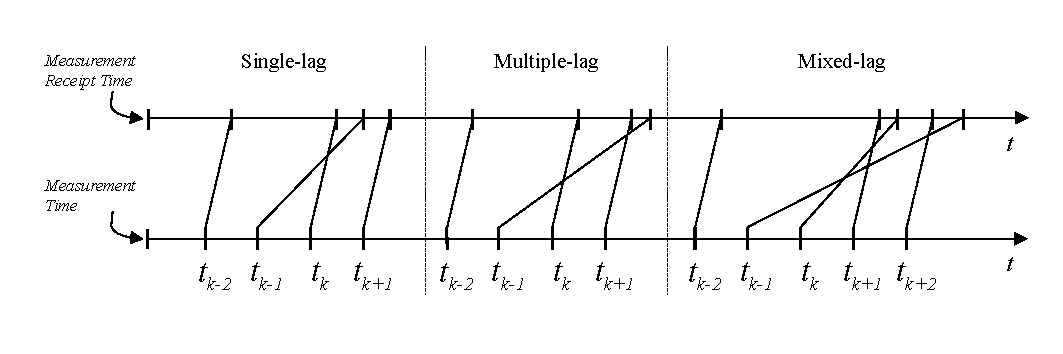
\includegraphics[scale=0.85]{Imagens/oosm.pdf}
	\caption[esquemas]{Different classes of out-of-sequence measurements irregularities}
	\label{fig:oosm}
\end{figure} 

\citep{Anxi2005} describes four different filtering approaches to deal with OOSM: reprocessing, that stores filter results to rollback with the time-delayed measurement; data buffering, that holds a set of measurements, greater than maximum expected lag, to be sorted before filtering; discarding data, that neglects time-delayed measurements; and directly updating, that uses the delayed information to update current state estimate. \citep{Bar-Shalom2000} used the last approach to describe an optimal filter for the single-lag case.

A summary of causes and effects that time delay causes in an estimator are illustrated in Figure \ref{fig:diagrama_delay}.

\begin{figure}[!htb]
	\centering
	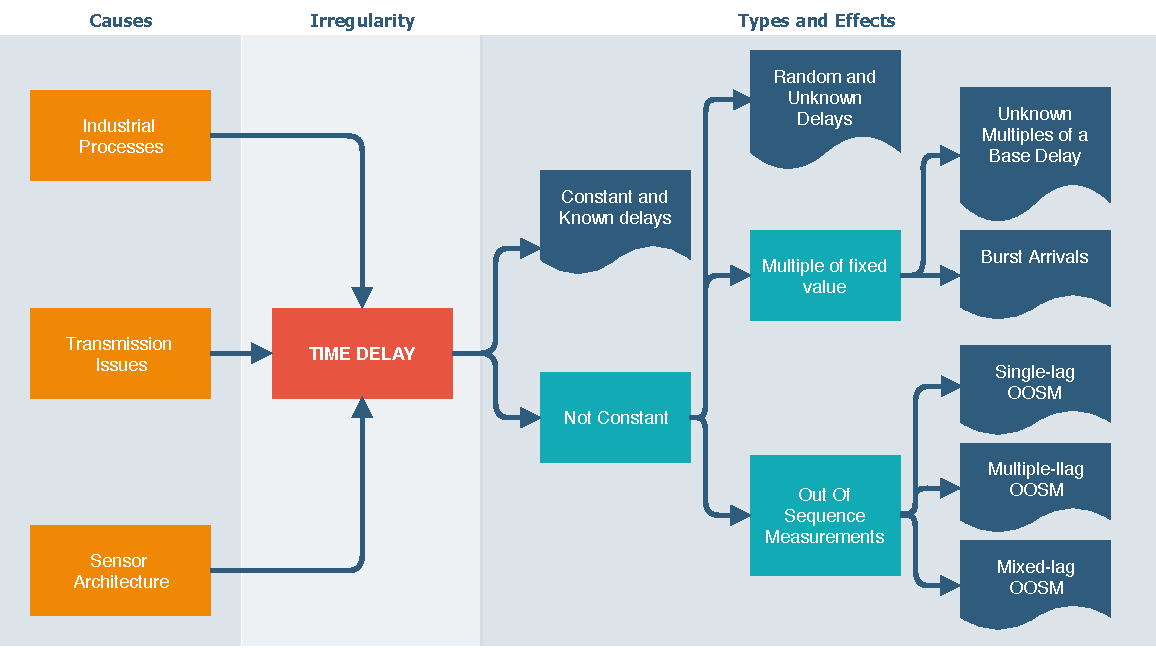
\includegraphics[scale=0.85]{Imagens/scheme_time-delay.pdf}
	\caption{Time delay diagram, showing the main causes (in orange) and effects (in dark blue) of time delay irregularity. The light blue boxes indicate different types that lead to different effects.}
	\label{fig:diagrama_delay}
\end{figure}

%\begin{figure}[!htb]
%	\begin{center}
%		
%		\begin{tikzpicture}[grow'=down,level distance=1.25in,sibling distance=.25in]
%		\tikzset{edge from parent/.style= 
%			{thick, draw, edge from parent fork down},
%			every leaf node/.style=
%			{draw,minimum width=1in,text width=1in,align=center,fill=orange!50},
%			every tree node/.style=
%			{draw,minimum width=1in,text width=1in,align=center,fill=blue!50}
%		}
%		
%		\Tree 
%		[.{Time Delay} 
%		{Transmission Issues} 
%		{Sensor Architecture} 
%		{Industrial Processes} 
%		]
%		
%		\end{tikzpicture}
%		
%	\end{center}
%	\caption{Irregular sampling diagram, showing the main causes (in orange) and effects (in blue) of irregularities}
%	\label{fig:diagrama_delay}
%\end{figure}	

\section{Packet Loss}

When data are being transmitted by a large network of sensors, there is a probability they can get lost in the way or they might arrive after a significant delay, which is equivalent to a loss for practical	 applications~\citep{Sinopoli2004}. Usually referred to as packet dropout/loss, missing or intermittent observations, they may happen due to node failures, network congestion, limited bandwidth or temporal failure. 
	
Mathematical description of packet dropouts can be carried out recursively, as described in~\citep{Sun2011}, by

\begin{align}
\centering
\begin{split}
z(t)=H(t)x(t)+v(t), \\
y(t) = \xi(t)z(t)+(1-\xi(t))y(t-1),
\end{split}
\end{align}

\noindent
where $z(t) \in \mathbf{R}^m$ is the measured output transmitted to the estimator, $v(t) \in \mathbf(R)^m$ is white noise, $y(t) \in \mathbf{R}^m$ is the measurement received by the estimator and $\xi(t) \sim Ber(p)$ is a Bernoulli random variable that takes the value 1 with probability $p$ and 0 with probability $1-p$. That is, when $\xi(t)$ is 1, there is no packet dropout. If $\xi(t)$ is 0, however, the latest output is used at current time, in a recursive fashion.

Another way of describing multiple packet dropouts is by limiting the amount of consecutive dropouts ~\citep{ShuliSun2008}, where the received measurements are defined by

\begin{equation}
\begin{split}
y(t) = 	& \xi(t)z(t) + (1-\xi(t))\xi(t-1)z(t-1)+...\\
		& + (1-\xi(t))(1-\xi(t-1))...(1-\xi(t-N+1))z(t-N), N \geq 1,\\
\end{split}
\end{equation}

Such a model dictates that the measurement used by the estimator will be only the most recent available, and the amount of missing observations is limited to $N$. This conclusion can be drawn by the fact that

\begin{equation}
\xi(t)+(1-\xi(t))\xi(t-1) + ... + (1-\xi(t))(1-\xi(t-1))...(1-\xi(t-N+1)) = 1.
\end{equation}

A summary of causes and effects that time delay causes in an estimator are illustrated in Figure \ref{fig:packet_loss}.

\begin{figure}[!htb]
	\centering
	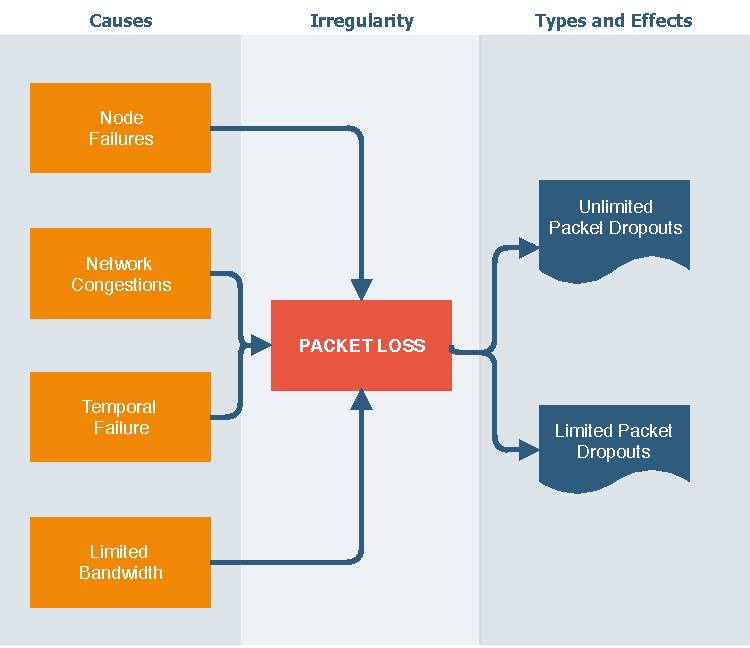
\includegraphics[scale=0.85]{Imagens/scheme_packet-loss.pdf}
	\caption{Packet loss diagram, showing the main causes (in orange) and effects (in dark blue) of time delay irregularity.}
	\label{fig:packet_loss}
\end{figure}


\section{Uncertain Observation}

For some applications, there is a chance that the observation signal sent to the estimator contains only noise. According to \citep{Jaffer1971}, it happens as a consequence of two situations: the observation was taken, but was lost during transmission, due to communication failures; or it was not transmitted at all, as it may happen for target tracking systems, for example, when the object being observed is not tracked at a sample time. An observation model for a sampled-data system can be described as

\begin{equation}
y(k) = \gamma(k)Cx(k) + Dv(k)
\end{equation}

\noindent
where $\gamma(k) \sim Ber(p(k))$ is a Bernoulli random variables, taking values of 0 or 1, with probabilities $p(k)$ and $1 - p(k)$, respectively.

Unlike the packet dropout problem, when the missing data are associated with the total absence of signal, the issue of uncertain observation has to be dealt with differently. A common approach is to detect the existence of signal prior to the assimilation, using a likelihood ratio test.  \citep{Middleton1968} proposes a joint approach to systematically detect and extract information from observation signals. If the estimator and detector are developed separately, te probability of false alarms is not used in the estimator, making it suboptimal. \citep{Nahi1969} developed an optimal recursive estimator, that uses the information of the random variable $\gamma$ in the algorithm, assuming it is independent and identically distributed. \citep{Hadidi1979} generalized the work of Nahi, for the case when the uncertainty of the signals presence is described by a Markovian sequence of binary random variables.

A summary of causes and effects that time delay causes in an estimator are illustrated in Figure \ref{fig:uncertain}.

\begin{figure}[!htb]
	\centering
	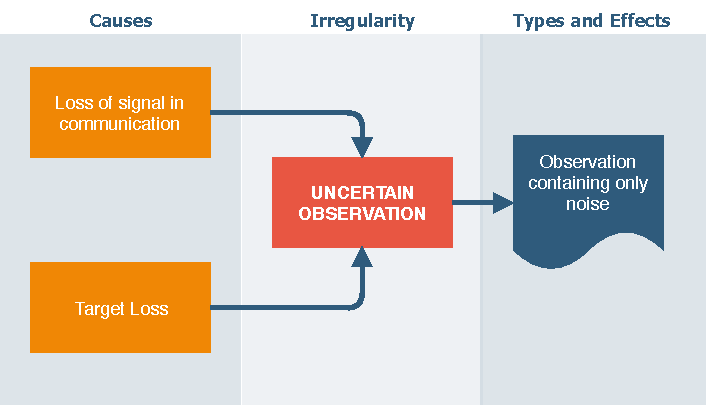
\includegraphics[scale=0.85]{Imagens/scheme_uncertain.pdf}
	\caption{Uncertain observations diagram, showing the main causes (in orange) and effects (in dark blue) of time delay irregularity.}
	\label{fig:uncertain}
\end{figure}

\section{Aperiodic Sampling}\label{sec:aperiodic}
	
All irregularities discussed so far may be present even in a periodic sampling scheme. However, for some applications, the sampling intervals are time-varying due to a variety of phenomena, causing what is called as aperiodic or asynchronous sampling. It can be the case of networked and embedded control systems, with unpredictable networked-induced issues, like irregular faults on samplers, oscillated loads, intermittent saturation or even variations in system components or parameters \citep{Shen2016}. Some imperfections may cause what is known as sampling jitter noise, which leads to time intervals being almost uniform. Automotive applications, radar imaging or event controlled systems are a few examples. In them, jitter noise happens due to sampling frequency similar to clock frequency, sampling requests delayed by the network or imperfect synchronization \citep{Eng2005}. For networks with a large amount of unsynchronized sensors, measurement arrival time intervals are randomly spaced and can be modeled as a stochastic process \citep{Micheli2002}. 

Sometimes, the system being observed has particularities that causes the aperiodic sampling. One example is seismology, where the spatial coordinates are irregularly sampled, because of natural obstacles \citep{Marvasti2001}. Other large scale systems, such as power grids, have sensors with a huge geographical separations, and different communication links to the estimation hub, which causes multiple and random inter-observation intervals \citep{Yan2017}.

Whereas for most cases, the non-uniformities in sampling time intervals appear as unwanted effects, there are cases when the sampling rule is designed to work irregularly. If there are limitations of communication resources (limited bandwidth or computation capacity) or a need for a reduced energy consumption, for example, time-driven sampling might be neglected in favor of an event-based scheme. In such strategy, an event-triggering mechanism is responsible for determining the sampling instants, according to Figure~\ref{fig:event-based}. For time-driven schemes, a clock triggers the transmission instants (a), while event-driven sampling instants depends on the sensor output itself with an optional feedback loop from the estimator, to assess estimation performance. Therefore, the trigger mechanism design provides a trade-off between performance and resource consumption efficiency, attracting a lot of research interest \citep{Liu2014}. The most common strategy for event-driven state estimation is the send-on-delta (SOD) \citep{Miskowicz2006}, which triggers the transmission when the value of the measured state deviates from the previous assimilated observation by an interval $\pm \Delta$, with $\Delta>0$. Other strategies were studied in \citep{Zou2017}. To avoid the risk of unexpected high amount of triggered measurements in a short period of time, which can lead to the dreaded Zeno behavior \citep{Tabuada2007}, lower-bounds can be defined both for the $\Delta$ value or for some explicit minimum inter-event time. 

\begin{figure}[!htb]
	\centering
	\begin{subfigure}
		\centering
		\text{(a)}\\
		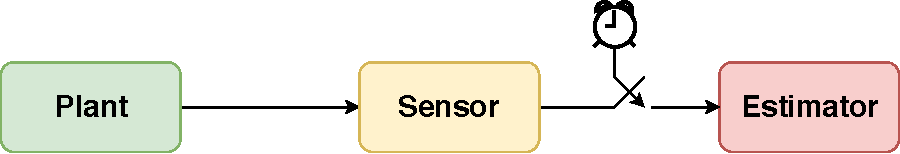
\includegraphics[width=0.75\textwidth]{Imagens/Event-based_clock.pdf}	
		\label{fig:evtb1}
	\end{subfigure}
	\vspace{1cm}\\
	\begin{subfigure}
		\centering
		\text{(b)}\\
		\vspace{0.25cm}
		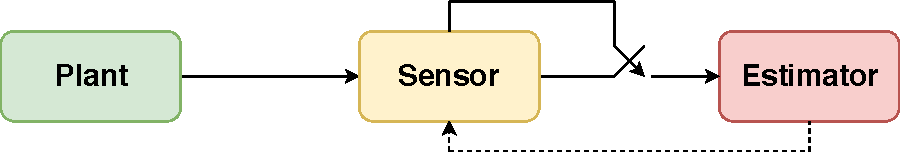
\includegraphics[width=0.75\textwidth]{Imagens/Event-based.pdf}
		%		\caption{}
		\label{fig:evtb2}
	\end{subfigure}
	\caption[Entradas]{Time-driven (a) and event-driven (b) sampling schemes. The connection between sensor and estimator is triggered by different mechanisms.}
	\label{fig:event-based}
\end{figure}

The measurement model of a linear system with aperiodic sampling can be defined as

\begin{equation}\label{eq:aperiodic}
y(t_k) = H(t_k)x(t_k) + v(t_k)
\end{equation}

\noindent
where $t_k$ is the random sampling time instant and the observation model matrix $H(t_k)$ is time-varying, if derived from the discretization of a continuous time system.

Generalizations of aperiodic sampling can be divided in two categories, based on how the estimator perceives the irregularity: as time noise added to a periodic pattern; or as a stochastic process, according to Figure~\ref{fig:aper-samp}. 

\begin{figure}[!htb]
	\centering
	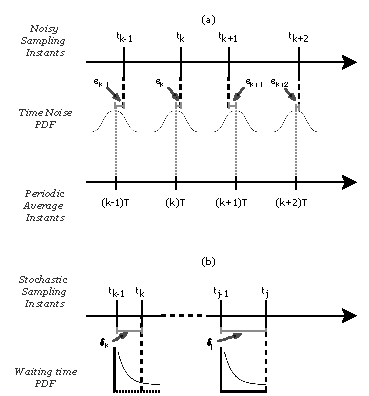
\includegraphics[width=0.85\textwidth]{Imagens/noisy_stoch_samp.pdf}	
	\caption[Entradas]{Aperiodic sampling categories: (a) noisy sampling over periodic intervals, with a Gaussian random variable added to expected time instants $kT$; and (b) sampling instants modeled as a stochastic process, with time intervals characterized by an exponential random variable (cumulative distribution functions are shown, for different $\lambda$ parameter values.)}
	\label{fig:aper-samp}
\end{figure}

For the first case, random time instants $t_k$ and the random time intervals $\delta_k$ can be defined as:

\begin{equation}
\begin{split}
t_k & \triangleq kT + \epsilon_k, \\
\delta_k & \triangleq t_k - t_{k-1} 
\end{split}
\end{equation}

\noindent
where $t_k$ is the k\textsuperscript{th} sampling instant, $T$ is the periodic time interval and $\epsilon_k$ is the deviation from the expected value $kT$. Note that, if the sampling time instants are a sequence of i.i.d Gaussian random variables, with variance $\sigma^2$, that is $t_k \sim \mathcal{N} (kT, \sigma^2)$, $\forall k \sim \mathbb{N}$, then the time interval random variable is Gaussian, with expected value $T$ and variance $2\sigma^2$, that is $\delta_k \sim \mathcal{N}(T,2\sigma^2)$.

For the stochastic process generalization, sampling time instants $t_k$ can be defined by the random time intervals $\delta_k$, such as:

\begin{equation}
\begin{split}
\delta_k & \triangleq t_k - t_{k-1}, \\
\delta_0 & \triangleq t_1
\end{split}
\end{equation}

\noindent
where random time intervals $\delta_k$ can be modeled, in the most flexible way, as a gamma probability density function, that is $\delta_k \sim \Gamma(k,\theta)$. If the shape parameter $k$ is a positive integer, it becomes an Erlang distribution, as used in \citep{Kanchanaharuthai2002}. For the most common case, where $k$ is held constant, the random time interval $\delta_k$ follows an exponential pdf the time sequence $t_k$ is represented by a Poisson stochastic process \citep{Micheli2002}.

A summary of causes and effects that time delay causes in an estimator are illustrated in Figure \ref{fig:aperiodic}.

\begin{figure}[!htb]
	\centering
	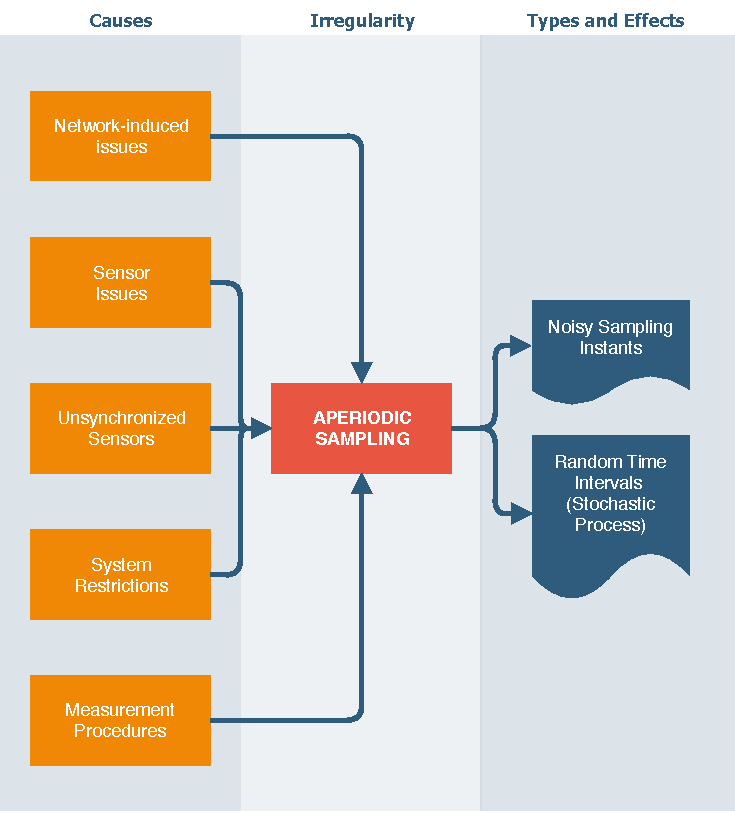
\includegraphics[scale=0.85]{Imagens/scheme_aperiodic.pdf}
	\caption{Uncertain observations diagram, showing the main causes (in orange) and effects (in dark blue) of time delay irregularity.}
	\label{fig:aperiodic}
\end{figure}

\section{Multi-Rate Sampling}

The last irregularity discussed is the multi-rate sampling. Generally, it refers to multiple sensors measuring the same system at different sampling rates. Many industrial processes need to control challenging variables that can be measured by online instruments that provide regular, fast rate and delay free information, but with low precision. Therefore, more accurate data are needed and usually available after slow and irregular laboratory analysis \citep{Penarrocha2012, Fatehi2017}. The combination of both sources of measurements leads to a multi-rate sampling scenario. 

A more common approach is the use of various sensors measuring the same physical information, to obtain better estimates, which has been drawing attention from real world applications, such as target tracking, robotics, surveillance and military. For such strategy, the sampling rates perceived by the estimator are often different from one another. The work of \citep{Lin2016} and the references therein provide a wide coverage of scenarios derived from multi-sensor multi-rate systems. 

Figure \ref{fig:multi-rate} illustrates the ways multi-rate sampling can manifest in a system. The different rates from the various sensor devices can be periodic (a), aperiodic (b) or even a mixture of both, as is the case for most industrial applications with laboratory analysis.

\begin{figure}[!htb]
	\centering
	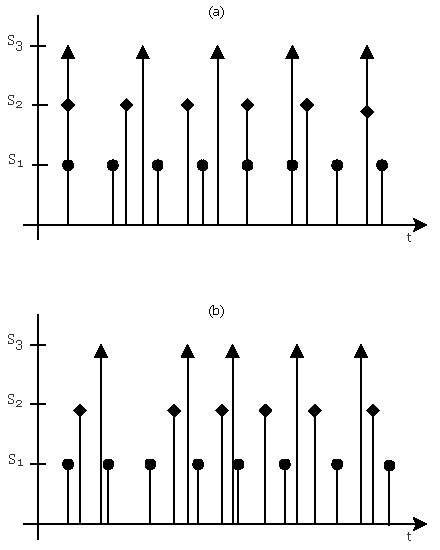
\includegraphics[width=0.5\textwidth]{Imagens/multi_rate.pdf}	
	\caption[Entradas]{(a) Periodic multi-rate and (b) aperiodic sampling scheme.}
	\label{fig:multi-rate}
\end{figure}

Aperiodic sampling rates can be described the same way as in Section \ref{sec:aperiodic}, by equation \ref{eq:aperiodic}. Periodic multi-rate measurements can be modeled as

\begin{equation}
	y_i(k_i) = H_i(x(k_i)) + v_i(k_1)
\end{equation}

\noindent
where $y_i(k_i)$ represents the $k_i^{th}$ observation from sensor $i$ and $H_i$ is the discrete measurement model matrix.

A summary of causes and effects that time delay causes in an estimator are illustrated in Figure \ref{fig:multi_rate}.

\begin{figure}[!htb]
	\centering
	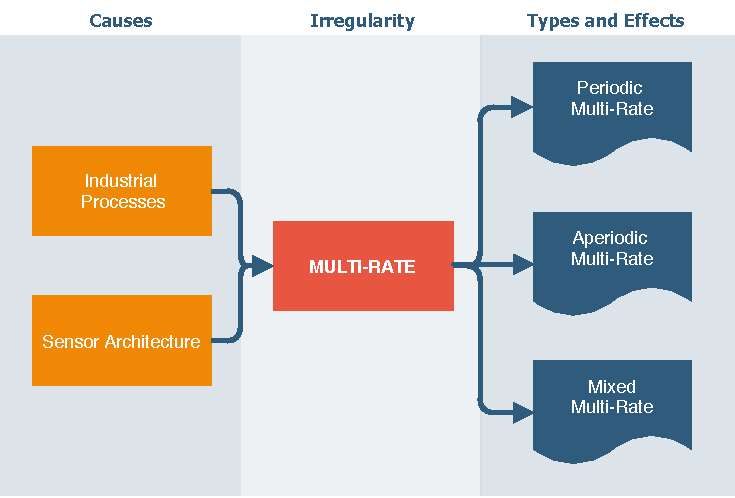
\includegraphics[scale=0.85]{Imagens/scheme_multi-rate.pdf}
	\caption{Uncertain observations diagram, showing the main causes (in orange) and effects (in dark blue) of time delay irregularity.}
	\label{fig:multi_rate}
\end{figure}


\clearpage
\clearpage
\thispagestyle{empty}
\cleardoublepage

%%--------------------------------------------------------------------
%Cap�tulo 3 - Methods
%------------------------------------------------------------------------------
\hypertarget{lcap3}{}
\chapter{Irregular Sampling}
\vspace{-1cm} \label{cap3}

%\begin{flushright}
%\begin{minipage}{0.7\linewidth}
%\emph{``Quando uma criatura humana desperta para um grande sonho e
%sobre ele lan�a toda a for�a de sua alma, todo o universo conspira a
%seu favor.''}
%\end{minipage}
%\end{flushright}
%
%\begin{flushright}
%{Goethe}
%\end{flushright}

%\vspace{1cm}

%%Colocar uma descri��o do cap�tulo aqui!
%\section{Introdu��o}\label{sec int_cap_2}

In the last chapter, we reviewed the main motivations and advantages behind the sensor fusion field of science, as well as its techniques. Despite all the growth and benefits obtained by fusing data from multiple sensors, some challenges naturally appear. For the state estimation problem for sampled-data systems, a common challenge is related to sampling irregularities introduced in a network.

In this chapter, we review the irregular sampling problem. First, the concept of irregular sampling adopted in this study is discussed. In Section \ref{sec:intro} we categorize the different types of irregularities that may occur in sampling and discuss their main causes and characteristics. Then, in Secton~\ref{sec:irreg_types}, each irregularity is further discussed, with examples, mathematical models and their subdivisions, where applicable. We end this chapter with a discussion of time synchronization in Section~\ref{sec:sync}, which is needed to guarantee a common time scale for all nodes in a network, enabling the irregularities to be dealt with appropriately.

\section{Definition of Irregular Sampling}

Most of the systems studied in estimation and control theories take place in an analog environment with dynamics evolving according to continous-time differential equations. However, due to the many benefits of digital technology implementations, their signal must be sampled in order to be processed, giving rise to the so-called \textit{sampled-data systems}. 

In practice, the sampling process is modeled by a sampler and a data hold device, that enables signal reconstruction. The most common data hold configuration is the zero-order holder (ZOH), that outputs a constant value equals to the signal value at the sampling instant during the whole time interval, until the next sample is available. 
%Therefore, the output of a sampler that transmits data every $T$ seconds and a ZOH is given by~\citep{Phillips1995}
%
%\begin{equation}\label{eq:sampled}
%\bar{f}(t)=f(0)[u(t)-u(t-T)]+f(T)[u(t)-u(t-2T	)]+f(2T)[u(t-2T)-u(t-3T)]+ \ ...,
%\end{equation}
%
%\noindent
%where $\bar{f}(t)$ represents the reconstructed sampled signal, $f(t)$ is the original continuous-time signal and $u(t)$ is the unit-step function. Taking the Laplace transform of (\ref{eq:sampled}) we have
%
%\begin{align}\label{eq:sampled_laplace}
%\bar{F}(s)=\mathcal{L}[f(t)]&=f(0)\left[\frac{1}{s}-\frac{e^{-Ts}}{s}\right]+f(T)\left[\frac{e^{-Ts}}{s}-\frac{e^{-2Ts}}{s}\right] + f(2T)\left[\frac{e^{-2Ts}}{s}-\frac{e^{-3		Ts}}{s}\right] + \ ... \notag \\
%&= \left[\sum_{n=0}^\infty f(nT) e^{-nTs}\right] \left[\frac{1-e^{-Ts}}{s}\right].
%\end{align}
%
%Only the first term of (\ref{eq:sampled_laplace}) is dependent on $f(t)$ and thus can be interpreted as the sampler, whereas the second term represents the ZOH. Note that neither exists alone, since the real physical signal is composed by both terms. Taking the inverse Laplace transform of the sampler term yields
%
%\begin{equation}\label{eq:sampled_invlaplace}
%\mathcal{L}^{-1}\left[\sum_{n=0}^\infty f(nT) e^{-nTs}\right] = f(0)\delta(t)+f(T)\delta(t-T)+f(2T)\delta(t-2T)+ \ ... \ ,
%\end{equation}
%
%\noindent
%where $\delta(t)$ is the unit impulse function, also known as Dirac delta function. Although it does not represent a real signal, (\ref{eq:sampled_invlaplace}) is referred to as the \textit{ideal sampler}~\citep{Phillips1995}.

Thus the state observations of a sampled-data system can be modeled as

\begin{equation}\label{eq:reg_sampled_obs}
y(t) = g(x(kT),v(kT),kT), \quad \textrm{for } kT\leq t<(k+1)T,
\end{equation}

\noindent
where $g\!\!: \mathbb{R}^n \times \mathbb{R}^r \times \mathbb{R^+} \rightarrow \mathbb{R}^m $ represents the observation model, $x(kT) \in \mathbb{R}^n$ is the state vector, $v(kT) \in \mathbb{R}^m$ is the measurement error, $k \in \mathbb{N}$ is the discrete-time index and $T \in \mathbb{R^+}$ is the sampling interval. 

Therefore, a sampled-data system is regularly sampled if its observation model can be modeled by (\ref{eq:reg_sampled_obs}), as a consequence of an \textit{ideal sampler}. In other words, in this study we refer to \textit{regular sampling} as measurements being taken periodically, with single-rate and transmitted without time-delay and any loss of information. Anything else will be framed as \textit{irregular sampling}.

\section{Contextualization}\label{sec:intro}

Sampling irregularities may occur due to a variety of issues. Sometimes they occur as undesired side effects of using large sensor networks architectures and others due to deliberate non-uniform sampling schemes. In this section we try to categorize and review the main irregularities observed in practice. The diagram in Figure \ref{fig:diagrama2} provides a simplified overview of them, separated by their sources.

\begin{figure}[!htb]
\centering
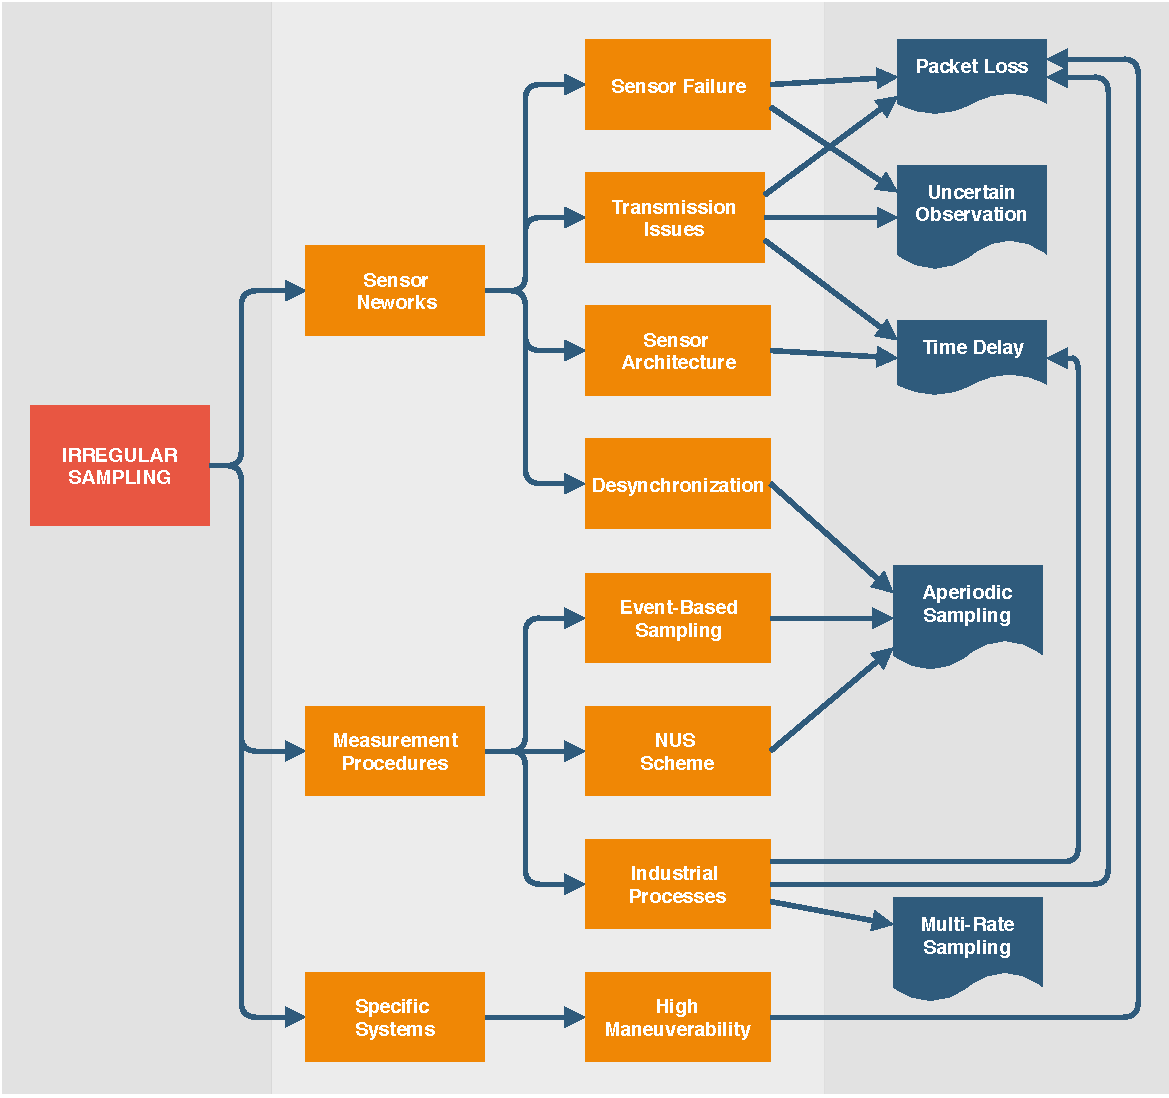
\includegraphics[width=\textwidth]{Imagens/irreg_sampling.pdf}
\caption[Irregular sampling diagram]{Irregular sampling diagram, showing the main causes (in orange) and effects (in blue)}
\label{fig:diagrama2}
\end{figure}

The use of imperfect communication networks seems to be the main cause of irregular sampling. Unreliable communication channels may lead to random time delays and loss of information, specially if data are transmitted using a common medium \citep{Sahebsara2007, Moayedi2011}. In case they get randomly interrupted during transmission or if a sensor fails at some point, the signal received may predominantly contain noise, causing uncertain observation or packet dropouts \citep{Hadidi1979, Wang2009}. Systems that are observed by a large number of desynchronized sensors will provide observations at random time intervals \citep{Micheli2002}. If they are synchronized but designed to operate in a centralized fashion, there is a chance that different time delays are produced due to distinct transmission routes for each sensor \citep{Bar-Shalom2000, Challa2003, Anxi2005}. 

However, the communication networks shall not always be held responsible. Some applications are designed to be measured in an irregular way. In event-based schemes, for example, the measurements are transmitted only when certain conditions are met \citep{Liu2014,Zou2017}. Such approach can reduce communication resource consumption substantially \citep{Hu2017}, but it will cause aperiodic sampling. Non-Uniform Sampling (NUS) is also intentionally used as an alias detection method \citep{Kunoh2015} or to enhance the spectral resolution of signals, largely used in Nuclear Magnetic Resonance (NMR) spectroscopy analysis \citep{Hyberts2013}, for instance. In other situations, due to the nature of the process being observed, the measurement strategy relies on different procedures. For a lot of chemical processes, for instance, the variables can be measured in an online, fast rate and delay free fashion, but providing inaccurate data. Therefore, laboratory analyses are used to improve estimation quality, but  usually at slower rates, sometimes irregularly and with possible time delays \citep{Fatehi2017}. Other industrial applications suffer from the same dilemma, and the sampling scheme ends up with a multi-rate data transmission, with random time delays and possibly measurement scarcity \citep{Penarrocha2012}. 


Finally, sampling irregularities might also appear due to a specific nature of a system. In some high maneuverable target-tracking applications, for example, there is a chance that the sensor misses the target, transmitting only noise, leading to the so called uncertain observation issue \citep{Wang2009, Chen2013}.

Whatever the reason for the irregularities, data need to be properly associated to the same observed phenomenon in order to be fused into knowledge. A crucial part of this association is the temporal synchronization of information on the time when the observations were taken \citep{Ping2003}. Most sensor fusion methods for irregularly sampled systems rely on the correct timestamps to develop modifications in classical algorithms. If observations are imprecisely time stamped, some alternatives have been proposed to incorporate some aspects of that imprecision in the estimation method \citep{Julier2005, Huck2011}. Still, some knowledge about the irregularity is assumed to be known. Alternatively, many techniques for time synchronization can be performed, to ensure a common temporal reference for all the sensors. 

On the next sections, we review the main irregular sampling types and the main approaches to deal with time synchronization in sensor networks.

\section{Types of Sampling Irregularity}\label{sec:irreg_types}

\subsection{Time Delay}

Signal time delays might affect state estimation in various ways and due to different reasons, as shown in Figure \ref{fig:diagrama_delay}. In some cases, delays can be modeled as constant and known \citep{Lu2005}. Alternatively they might not be known and constant, but still multiple of a fixed value. In such cases, observations might be received in a burst, when more than one packet arrive between two consecutive sampling instants. State estimation algorithms can be adapted to handle such irregularity by using only the latest measurement and discarding all others, or implementing a buffer to iterate over all received packets \citep{Moayedi2011}.

\begin{figure}[!htb]
	\centering
	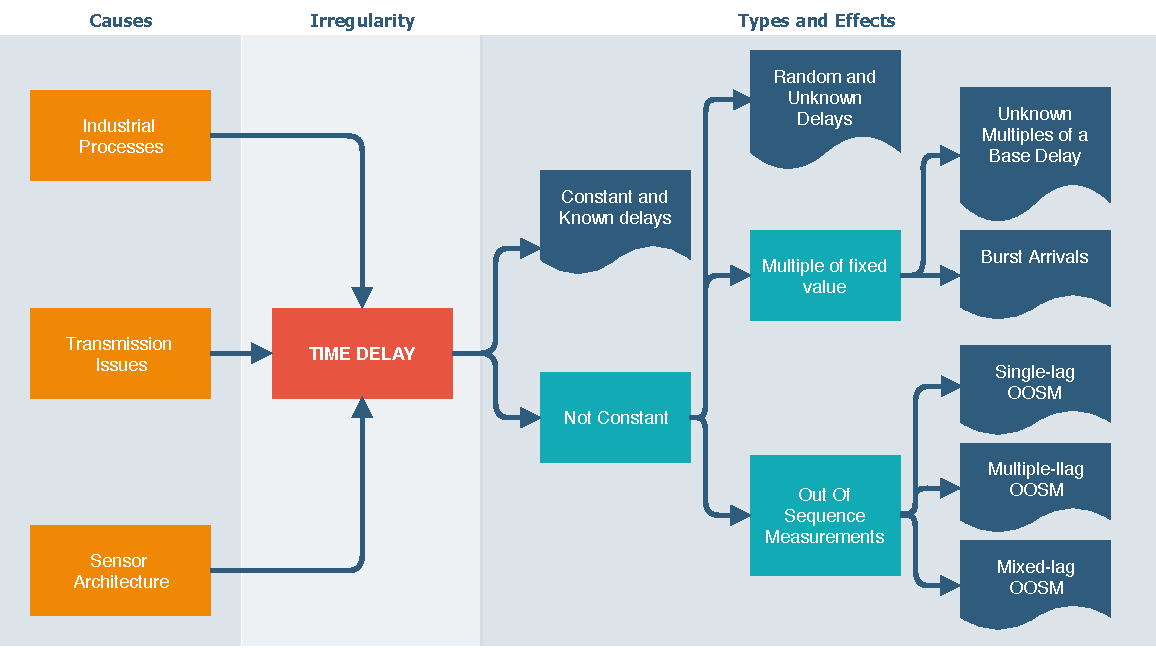
\includegraphics[width=\textwidth]{Imagens/scheme_time-delay.pdf}
	\caption[Time delay diagram]{Time delay diagram, showing the main causes (in orange) and effects (in dark blue) of time delay irregularity. The light blue boxes indicate different types that lead to different effects.}
	\label{fig:diagrama_delay}
\end{figure}

%Time-delay systems (TDS) are probably the most common mathematical representation to time delays in practice. The works of \citep{Richard2003, Fridman2014} and the references therein provide a good coverage of the subject. In TDSs, there might be delays in the input or in the output signals, introduced by communication networks, or even in the states themselves. The latter phenomenon is called system with aftereffect or dead-time. Since we are studying the irregular sampling issue, only signal delays are relevant to us. A summary of causes and effects that time delay causes in an estimator are illustrated in Figure \ref{fig:diagrama_delay}.

%Considering delays in the measurement model only, \citep{Lu2005} studied the estimation problem when they are constant and known. They describe a discrete linear measurement model observed by $l$ different systems with delays as 
%
%\begin{equation}\label{eq:delay_model}
%	y_i(kT)=H_i(kT)x(t_i)+v_i(kT)
%\end{equation}
%
%
%\noindent
%where $k$ is the discrete-time index of measurements, $T$ is the sampling interval, $i=0,\ 1,\ ...,\ l$ and $l$ is the number of different known delays for each observation system. $y_i(kT) \in \mathbb{R}^{p_i}$ are delayed measurements and $v_i(kT) \in \mathbb{R}^{p_i}$, the measurement noise. The known delayed time instants are given by $t_i=t_{i-1}-d_i$, with $d_0=0$, $d_i>0$ for $i>0$ and $t_0=kT$. For a given time instant $kT$, $y_i(kT)$ represents the observation of state $x(t_i)$ at time $kT$, with total delay $\sum_{k=1}^{i}d_k$. Thus, if $T \geq d_1 \ + \ ...\  + \ d_l$, the complee observation vector of state $x(t_i)$ at time $kT$, becomes $[y_0^T(kT) \ ... \ y_l^T(kT)]^T$. On the other hand, if the sampling interval is smaller than the delay of one or more observation system, that is $ d_1 \ + \ ... \ + \ d_{i-1}\leq T < d_1 \  + ... \ + \ d_l$, then observation of the system is given by $[y_0^T(kT) \ ... \ y_{i-1}^T(kT) \ 0 \ ... \ 0]^T$.
%



However, in many applications the measurements are received by the estimator with irregular and unknown delays, although taken at regular time intervals. In such cases, time delays can be interpreted as a stochastic process $d(k)$, varying randomly throughout time \citep{Han2009}.

% describes a discrete-time measurement model for random delayed observations as
%
%\begin{equation}\label{eq:delay_model2}
%y(k) = H(k)x(k-d(k))+L(k)v(k)
%\end{equation}
%
%\noindent
%where $d(k) \in \mathbb{N}$ is a random but bounded time delay, assumed to be a discrete-time Markov Chain with finite space $\{0,\ d\}$, observable at each sampling time $k$.

Multiples of a known lag or not, delayed measurements from a multisensor system can arrive disordely, which leads to the sampling irregularity commonly known as out-of-sequence-measurements (OOSM). It can be classified in three ways, depending on the number of lags, according to Figure~\ref{fig:oosm}. 

\begin{figure}[!htb]
	\centering
	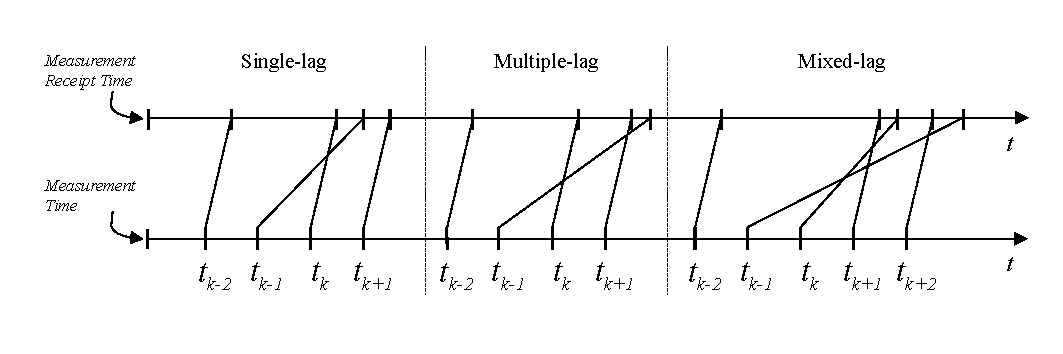
\includegraphics[width=0.95\textwidth]{Imagens/oosm.pdf}
	\caption{Different classes of out-of-sequence measurements irregularities}
	\label{fig:oosm}
\end{figure} 

\citep{Anxi2005} describes four different filtering approaches to deal with OOSM: reprocessing, that stores filter results to rollback with the time-delayed measurement; data buffering, that holds a set of measurements, greater than the maximum expected lag, to be sorted before filtering; discarding data, that neglects time-delayed measurements; and directly updating, that uses the delayed information to update current state estimate. \citep{Bar-Shalom2000} used the last approach to describe an optimal filter for the single-lag case.


\subsection{Packet Loss}

When data are being transmitted by a large network of sensors, there is a probability that they get lost in the way or they might arrive after a significant delay, which is equivalent to a loss for practical	 applications~\citep{Sinopoli2004}. Usually referred to as packet dropout or loss, missing or intermittent observations or scarse measurements~\citep{Albertos2004}, they may happen due to node failures, network congestion, limited bandwidth or temporal failure. A summary of causes and effects associated with packet loss are shown in Figure \ref{fig:packet_loss}.

\begin{figure}[!htb]
	\centering
	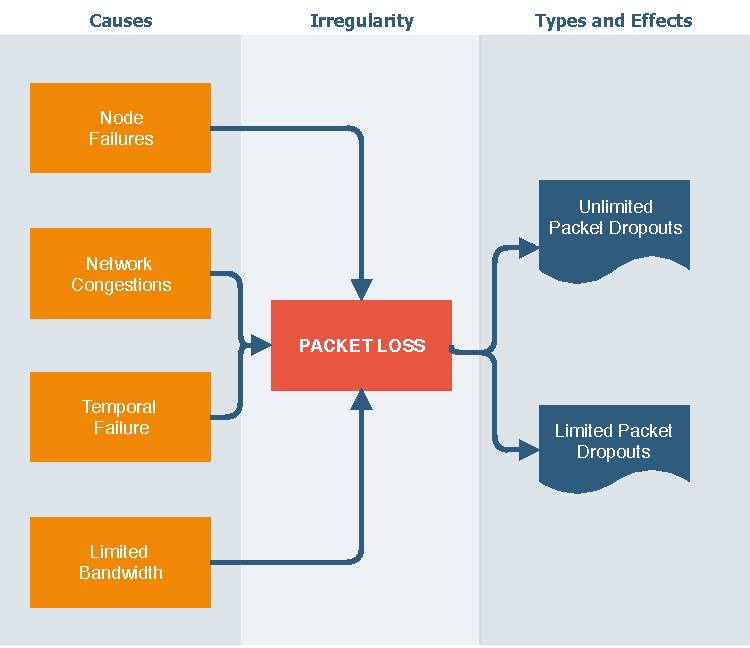
\includegraphics[width=0.75\textwidth]{Imagens/scheme_packet-loss.pdf}
	\caption[Packet loss diagram]{Packet loss diagram, showing the main causes (in orange) and effects (in dark blue) of time delay irregularity.}
	\label{fig:packet_loss}
\end{figure}

	
Mathematical description of packet dropouts can be carried out recursively, as described in~\citep{Sun2011}, by

\vspace{-2pt}
\begin{equation}
\centering
y(k)  = \xi(k)z(k)+(1-\xi(k))y(k-1),
\end{equation}

\noindent
where $z(k) \in \mathbb{R}^m$ is the $k$-th measured output transmitted to the estimator, $y(k) \in \mathbb{R}^m$ is the $k$-th measurement received by the estimator and $\xi(k) \sim Ber(p)$ is a Bernoulli stochastic process that takes the value 1 with probability $p$ and 0 with probability $1-p$. That is, when $\xi(k)$ is 1, there is no packet dropout. If $\xi(k)$ is 0, however, the latest output is used at current time, in a recursive fashion.

Another way of describing multiple packet dropouts is by limiting the amount of consecutive dropouts ~\citep{ShuliSun2008}, where the received measurements are defined by
\vspace{-1pt}
\begin{equation}
\begin{split}
y(k) = 	& \xi(k)z(k) + (1-\xi(k))\xi(k-1)z(k-1) + (1-\xi(k))(1-\xi(k-1))\xi(k-2)z(k-2)  +\ ...\\
		& + (1-\xi(k))(1-\xi(k-1))...(1-\xi(k-N+1))\xi(k-N)z(k-N), \quad N \geq 1.\\
\end{split}
\end{equation}

Such a model dictates that the measurement used by the estimator will be only the most recent available, and the amount of missing observations is limited to $N$. 

\subsection{Uncertain Observation}\label{sec:uncertain}

For some applications, there is a chance that the observation signal sent to the estimator contains only noise. According to \citep{Jaffer1971}, it happens as a consequence of two situations: the observation was taken, but it was lost during transmission, due to communication failures; or it was not transmitted at all, as it may happen for target tracking systems, for example, when the object being observed is not tracked at a sample time. A summary of causes and effects associated with uncertain observations are shown in Figure \ref{fig:uncertain}.

\begin{figure}[!htb]
	\centering
	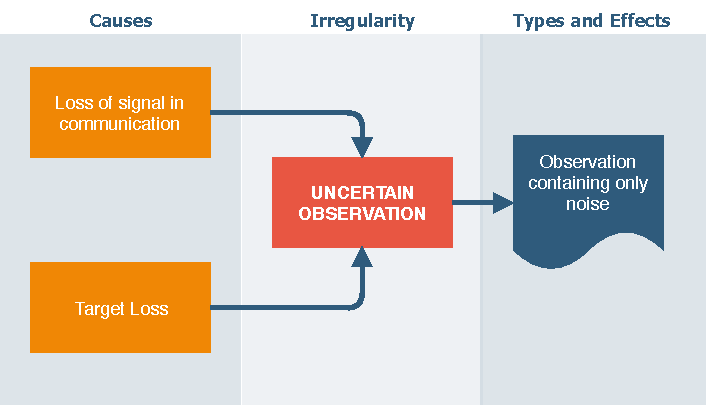
\includegraphics[width=0.75\textwidth]{Imagens/scheme_uncertain.pdf}
	\caption[Uncertain observations diagram]{Uncertain observations diagram, showing the main causes (in orange) and effects (in dark blue) of time delay irregularity.}
	\label{fig:uncertain}
\end{figure}

An observation model for a sampled-data system with uncertain observations can be described as

\begin{equation}
y(k) = \xi(k)z(k) + v(k)
\end{equation}

\noindent
where $z(k) \in \mathbb{R}^m$ is the $k$-th measured output transmitted to the estimator, $y(k) \in \mathbb{R}^m$ is the $k$-th measurement received by the estimator and $\xi(k) \sim Ber(p(k))$ is a Bernoulli random variables, taking values of 0 or 1, with probabilities $p(k)$ and $1 - p(k)$, respectively.

Unlike the packet dropout problem, when the missing data are associated with the total absence of signal, the issue of uncertain observation has to be dealt with differently. A common approach is to detect the existence of signal prior to the assimilation, using a likelihood ratio test.  \citep{Middleton1968} proposes a joint approach to systematically detect and extract information from observation signals. If the estimator and detector are developed separately, the probability of false alarms is not used in the estimator, making it sub-optimal. \citep{Nahi1969} developed an optimal recursive estimator that uses the information of the stochastic process $\xi(k)$ in the algorithm, assuming its sequence is independent and identically distributed. \citep{Hadidi1979} generalized the work of Nahi, for the case when the uncertainty of the signals presence is described by a Markovian sequence of binary random variables.



\subsection{Aperiodic Sampling}\label{sec:aperiodic}
	
All irregularities discussed so far may be present even in a periodic sampling scheme. However, for some applications, the sampling intervals are time-varying due to a variety of phenomena, causing the so-called aperiodic or asynchronous sampling. A summary of causes and types of aperodic sampling is presented Figure \ref{fig:aperiodic}.

\begin{figure}[!htb]
	\centering
	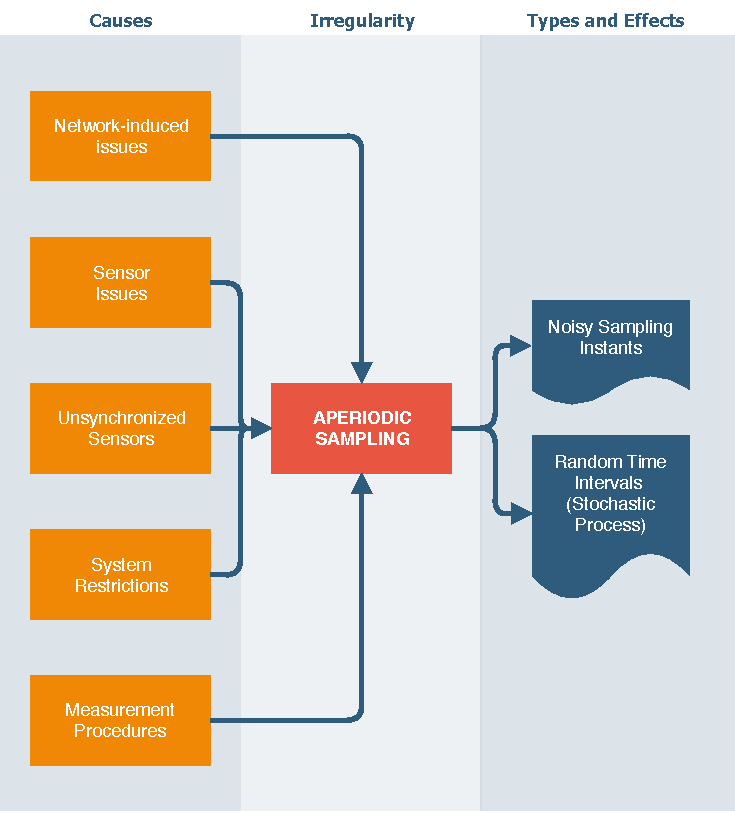
\includegraphics[width=0.75\textwidth]{Imagens/scheme_aperiodic.pdf}
	\caption[Aperiodic sampling diagram]{Aperiodic sampling diagram, showing the main causes (in orange) and types (in dark blue) of irregularity.}
	\label{fig:aperiodic}
\end{figure}

Usually such irregularity happens in networked and embedded control systems, with unpredictable networked-induced issues, such as irregular faults on samplers, oscillated loads, intermittent saturation or even variations in system components or parameters \citep{Shen2016}. Some imperfections may cause what is known as sampling jitter noise, which leads to time intervals being almost uniform. Automotive applications, radar imaging or event controlled systems are a few examples. In such cases, jitter noise happens due to a sampling frequency similar to the clock frequency; to sampling requests delayed by the network; or to imperfect synchronization \citep{Eng2005}. For networks with a large amount of unsynchronized sensors, measurement arrival time instants are randomly spaced and can be modeled as stochastic processes \citep{Micheli2002}. Sometimes, the system being observed has particularities that causes the aperiodic sampling. One example is seismology, where the spatial coordinates are irregularly sampled, because of natural obstacles \citep{Marvasti2001}. Other large scale systems, such as power grids, have sensors with huge geographical separations and different communication links to the estimation hub, causing multiple and random inter-observation intervals \citep{Yan2017}.

Whereas for most cases the variations in sampling time intervals appear as unwanted effects, there are cases when the sampling rule is designed to work aperiodically. If there are limitations of communication resources (limited bandwidth or computation capacity, for instance) or a need for reduced energy consumption, time-driven sampling might be replaced in favor of an event-based scheme. In such strategy, an event-triggering mechanism is responsible for determining the sampling instants, as depicted in Figure~\ref{fig:event-based}. For time-driven schemes, a clock triggers the transmission instants, while event-driven sampling instants depends on the sensor output itself with an optional feedback loop from the estimator to assess estimation performance. Therefore, the trigger mechanism design provides a trade-off between performance and resource consumption efficiency, attracting a lot of research interest \citep{Liu2014}. The most common strategy for event-driven state estimation is the send-on-delta (SOD) \citep{Miskowicz2006}, which triggers the transmission when the value of the measured state deviates from the previous assimilated observation by an interval $\pm \Delta$, with $\Delta>0$. Other strategies were studied in \citep{Zou2017}. To avoid the risk of unexpected high amount of triggered measurements in a short period of time, lower-bounds can be defined both for the $\Delta$-value or for some explicit minimum inter-event time.



\begin{figure}[!htb]
	\centering
	\begin{subfigure}
		\centering
		\text{(a)}\\
		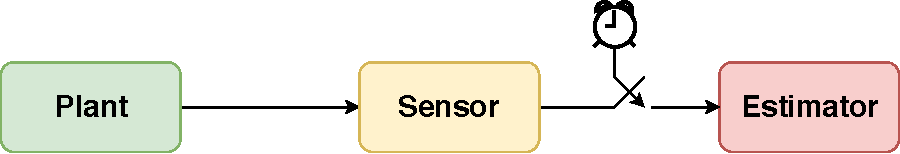
\includegraphics[width=0.75\textwidth]{Imagens/Event-based_clock.pdf}	
		\label{fig:evtb1}
	\end{subfigure}
	\vspace{1cm}\\
	\begin{subfigure}
		\centering
		\text{(b)}\\
		\vspace{0.25cm}
		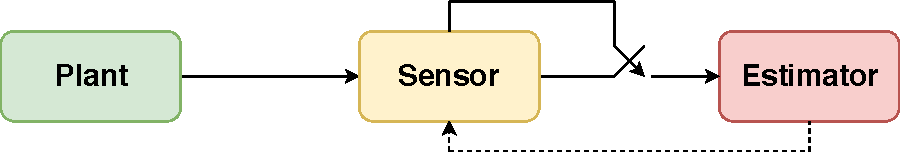
\includegraphics[width=0.75\textwidth]{Imagens/Event-based.pdf}
		%		\caption{}
		\label{fig:evtb2}
	\end{subfigure}
	\caption[Time-driven and event-driven sampling schemes]{(a) Time-driven and (b) event-driven sampling schemes. The connection between sensor and estimator is triggered by different mechanisms.}
	\label{fig:event-based}
\end{figure}




The measurement model with aperiodic sampling can be defined as

\begin{equation}\label{eq:aperiodic}
y(t_k) = z(t_k) + v(t_k)
\end{equation}

\noindent
where $t_k$ is the random sampling time instant and $z(t_K)$ is the transmitted measurement.

Generalizations of aperiodic sampling can be divided in two categories, based on how the estimator perceives the irregularity: as time signal noise added to a periodic pattern; or as a stochastic process, as illustrated in Figure~\ref{fig:aper-samp}. 

\begin{figure}[!htb]
	\centering
	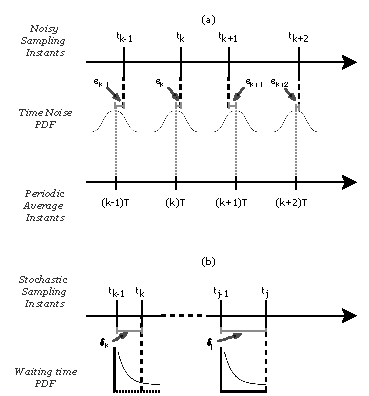
\includegraphics[width=0.8\textwidth]{Imagens/noisy_stoch_samp.pdf}	
	\caption[Two models of aperiodic sampling]{Two models of aperiodic sampling: (a) noisy sampling over periodic intervals, with a Gaussian random variable added to expected time instants $kT$; and (b) sampling instants modeled as a stochastic process, with time intervals characterized by an exponential random variable. For (b), the cumulative distribution functions are shown, for different $\lambda$ parameter values.}
	\label{fig:aper-samp}
\end{figure}

For the first case, random time instants $t_k$ and the random time intervals $\delta_k$ can be defined as:
\vspace{-1pt}
\begin{equation}
\begin{split}
t_k & \triangleq kT + \epsilon_k, \\
\delta_k & \triangleq t_k - t_{k-1} 
\end{split}
\end{equation}

\noindent
where $t_k$ is the $k$\textsuperscript{th} sampling instant, $T$ is the constant time interval and $\epsilon_k$ is the deviation from the expected value $kT$. Note that, if the sampling time instants are a sequence of i.i.d Gaussian random variables, with variance $\sigma^2$, that is $t_k \sim \mathcal{N} (kT, \sigma^2)$, $\forall k \sim \mathbb{N}$, then the time interval random variable is Gaussian, with expected value $T$ and variance $2\sigma^2$, that is $\delta_k \sim \mathcal{N}(T,2\sigma^2)$.

For the stochastic process generalization, sampling time instants $t_k$ can be defined by the random time intervals $\delta_k$, such as:

\begin{equation}
\begin{split}
\delta_k & \triangleq t_k - t_{k-1}, \\
\delta_0 & \triangleq t_0
\end{split}
\end{equation}

\noindent
where random time intervals $\delta_k$ can be modeled, in the most flexible way, as a gamma probability density function, that is $\delta_k \sim \Gamma(\kappa,\theta)$. If the shape parameter $\kappa$ is a positive integer, then it becomes an Erlang distribution, as done in \citep{Kanchanaharuthai2002}. For the most common case, where $\kappa$ is held constant, the random time interval $\delta_k$ follows an exponential PDF and the time sequence $t_k$ is represented by a Poisson stochastic process \citep{Micheli2002}. In fact, Micheli and Jordan proved that for a network with $N$ unsynchronized sensors with sampling period $T$, the waiting time between two arrivals tends, in distribution, to the exponential random variable, that is 
$\delta_k \sim \mathcal{E} (\lambda)$, where $\lambda = N/T$, as $N$ tends to infinity. In such cases, the expected value of the RV $\delta_k$ is $E[\delta_k] = 1/\lambda$ and its variance is $Var[\delta_k] = 1/\lambda^2$.


\subsection{Multi-Rate Sampling}

The last irregularity discussed is the multi-rate sampling. Generally, it refers to multiple sensors measuring variables from the same system at different sampling rates. Figure \ref{fig:multi_rate} shows a schematic of causes and effects associated with multi-rate sampling irregularity.

\begin{figure}[!htb]
	\centering
	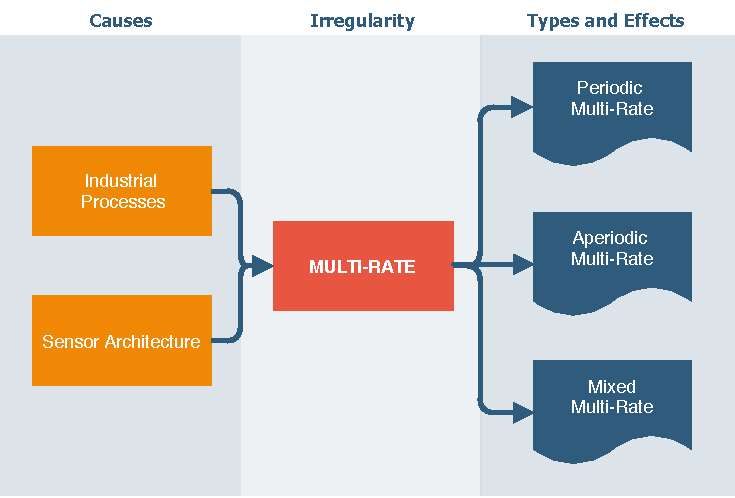
\includegraphics[width=0.75\textwidth]{Imagens/scheme_multi-rate.pdf}
	\caption[Multi-rate sampling diagram]{Multi-rate sampling diagram, showing the main causes (in orange) and types (in dark blue) of multi-rate sampling.}
	\label{fig:multi_rate}
\end{figure}

Many industrial processes need to control variables that can be measured by online instruments that provide regular, fast rate and delay free information, but with low precision. Therefore, more accurate data are needed and usually available after slow, irregular and human-dependent laboratory analysis \citep{Penarrocha2012, Fatehi2017}. The combination of both sources of measurements leads to a multi-rate sampling scenario. 

A more common approach is the use of various sensors measuring the same physical information, to obtain better estimates, which has been drawing attention from real world applications, such as target tracking, robotics, surveillance and military. For such strategy, the sampling rates perceived by the estimator are often different from one another. The work of \citep{Lin2016} and the references therein provide a wide coverage of scenarios derived from multi-sensor multi-rate systems. 

Figure \ref{fig:multi-rate} illustrates the ways multi-rate sampling can be manifested in a system. The different rates from the various sensor devices can be periodic (a), aperiodic (b) or even a mixture of both, as it is the case for most industrial applications with laboratory analysis.

\begin{figure}[!htb]
	\centering
	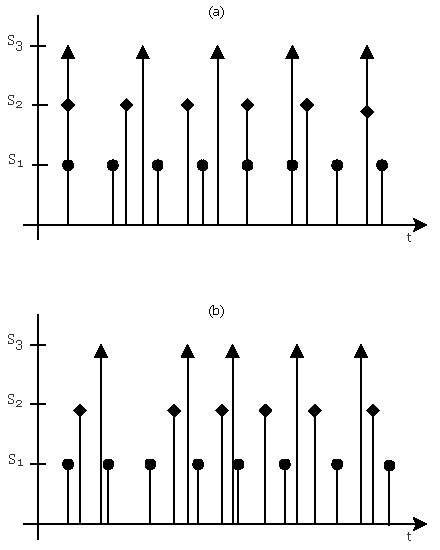
\includegraphics[width=0.5\textwidth]{Imagens/multi_rate.pdf}	
	\caption[Periodic and aperiodic multi-rate sampling scheme]{(a) Periodic and (b) aperiodic multi-rate sampling scheme. Labels $S_1$, $S_2$, $S_3$ refer to the sampling instants of three different sensors, from the highest sampling rate to the lowest sampling rate.}
	\label{fig:multi-rate}
\end{figure}

Aperiodic sampling rates can be described the same way as in Section \ref{sec:aperiodic}. Periodic multi-rate measurements can be modeled as

\begin{equation}
	y_i(k_iT_i) = z(k_iT_i) + v_i(k_iT_i)
\end{equation}

\noindent
where $y_i(k_iT_i)$ represents the $k_i^{th}$ observation from sensor $i$ with periodic sampling rate $T_i$ and $z(k_iT_i)$ is the $k$-th transmitted measurement of the $i$-th sensor.

\section{Time Synchronization}\label{sec:sync}

There are techniques to handle all the irregularities discussed in this chapter and still achieve efficient state estimation performance. Provided that the estimator is able to use the information on the time that measurements were taken, there are many algorithms that provide interesting results. 

In general, multi-sensor data fusion techniques for state estimation require that exact measurement timestamps are available in order to assimilate data properly \citep{Ping2003, Brahmi2013}. However, that is not always the case and situations may arise in which timestamps were not collected or their values are unreliable. Examples of the latter may occur when measurements are time stamped when they are received by the estimator instead of being time stamped at the moment it was taken, or when they are time stamped using temporal information from local clocks without centralized synchronization \citep{Julier2005}. 

In many practical applications, if sampling irregularity cannot be accounted for accordingly, data are fused using the time of arrival as timestamp \citep{Huck2011}, or irregularities such as OOSM are just disregarded completely \citep{Kwok2004}. The effects of such neglect has seldom been investigated, however. In one of the few studies, \citep{Julier2005} considered the state estimation problem for delayed but periodic observations with imprecise and unknown timestamps, with the assumption that they could be statistically characterized. They proposed an implementation of the covariance union (CU) technique, using the timestamp statistics in the filter update step. First, the method calculates the updates considering both the maximum and minimum expected delayed and then merged both results with a convex combination designed to minimize the state covariance matrix. CU algorithm was tested for the problem of estimating the states of a linear system, considering a random time delay, uniformly distributed between 2 and 10 time steps. Estimation performance was tested against four other methods: \textit{known delay}, that considers the time delay to be known perfectly, as a baseline for comparison; \textit{mean delay}, that assumes the delay to be always an average of 6 time steps; maximum likelihood, that calculates the likelihood of each possible time step and selects the highest; and Probabilistic Data Association Filter (PDAF) \citep{Bar-shalom2009}, that also calculates the likelihood of each step and averages the results using the likelihood as weight. They used the normalized state estimation error (NEES) test for consistency assessment, which we explain later in Section~\ref{sec:metrics}, for a linear system with two states. Therefore, the expected value of NEES for a consistent filter should be 2. The results are replicated in Table~\ref{tab:cu_consistency} for all algorithms. 

\begin{table}[!ht]
	\centering
	\setlength{\tabcolsep}{12pt}
	\caption[Consistency test results for fusion of time delayed measurements with uncertain timestamps]{Comparison of NEES consistency test results for fusion of time delayed measurements with uncertain timestamps for a linear system with two states}
	\renewcommand{\arraystretch}{1.5}
	\begin{tabular}{l  c }
		\toprule
		Method				& E$\left[\textrm{NEES}\right]$  \\
		\midrule
		Known delay 		& 1.9992  \\
		Mean delay 			& 37.6949  \\
		Max likelihood 		& 54.9323 \\
		Covariance union 	& 1.3172 \\
		PDAF & 1.8749 \\
		\bottomrule
	\end{tabular}
	\label{tab:cu_consistency}
\end{table}

As expected, the method with known delay was the most consistent, that is with $E\left[ \textrm{NEES} \right]$ results closer to 2. CU and PDAF were both consistent, with slightly overestimated state error. They argued that, although PDAF obtained better consistency results, it has significantly higher computational costs. Nevertheless, the results of the mean delay and maximum likelihood are highly inconsistent, showing that the neglect or oversimplification of the imprecision in timestamp leads to considerable performance degradation.

Another approach to overcome unknown timestamps on the presence of sampling irregularities was studied by \citep{Kwok2004}. In the presence of OOSM, when sensor information is sampled at much faster rates than filter update rates, the real-time particle filter (RTPF) proposed by them makes efficient use of all sensor information, instead of discarding sensor readings. That is achieved by dividing the received measurements among sample sets and then representing the states as a mixture of those sets.

Alternatively, in order to avoid performance degradation, one can make use of time synchronization schemes, widely used in communication networks, to ensure global time stamps. Wireless sensor networks (WSN) are particularly dependent on such techniques, due to limited computation, energy and communication resources of the sensing devices used. The works of \citep{Sivrikaya2004} and \citep{Roemer2003} provide detailed reviews on the time synchronization problem in sensor networks. 

%They explain the problem through computer clock mechanism. 
%
%With the aid of a hardware oscillator, local clocks from a sensing device node $i$ approximates real time $t$ as $C_i(t)$ by
%	
%\begin{equation}\label{eq:clock1}
%C_i(t) = a_it+b_i
%\end{equation}
%
%\noindent
%where $a_i(t)$ is the clock \textit{drift}, that is the clock frequency, and $b_i(t)$ represents an \textit{offset} value, or the difference from real value $t$.
%
%Clock approximations from two nodes in a network are compared by
%
%\begin{equation}\label{eq:clock2}
%C_1(t) = a_{12}C_2(t)+b_{12}
%\end{equation}
%
%\noindent
%where $a_{12}$ is the relative \textit{drift} and $b_{12}$ is the relative offset between nodes. 
%
%Under equations (\ref{eq:clock1}) and (\ref{eq:clock2}), the synchronization problem becomes the equalization of the computer clocks from all different $n$ devices, in its most strict form. Thus, synchronization strategies can either match all clock frequencies and offsets once or perform repeated offset corrections over time. There are more relaxed versions of synchronizations, such as the one proposed by \cite{Roemer2003}, that aims at maintaining only the order of events.	

Probably the most popular time synchronization method is the one being used in the internet environment for years, the Network Time Protocol (NTP), designed by \citep{Mills1991}. For most control and WNS applications, however, it is not suitable, due to very different requirements, such as energy consumption, precision and scalability \citep{Ganeriwal2003}. 

Another easy solution would be to equip all sensing devices in the network with a global positioning system (GPS) for a global time synchronization, but such solution is very expensive, not energy efficient and its signal might not work properly in every environment.

Therefore, many alternative methods have been proposed, and the work of \citep{Kaur2015} updates the studies from \citep{Sivrikaya2004}, with an exploration of the most recent synchronization protocols for sensor networks, that is: reference broadcast synchronization (RBS) \citep{Elson2002}; timing-sync protocol for sensor networks (TPSN) \citep{Ganeriwal2003};  delay measurement time synchronization (DMTS) \citep{Ping2003}; lightweight tree-based synchronization (LTS) \citep{Greunen2003}; tiny-sync mini-sync \citep{Sichitiu2003}; flooding time synchronization protocol (FTSP) \citep{Maroti2004}; lightweight and energy efficient time synchronization (LEETS) \citep{MingxiaXu2005}; time diffusion protocol (TDP) \citep{Su2005}; and time synchronization based on spanning tree (TSST) \citep{He2008}. A comparison adapted from Kaur ad Abhilasha is presented in Table~\ref{tab:sync}.


\begin{table}[!htb]
	\renewcommand{\arraystretch}{1.3}
	\caption[Comparison of time synchronization methods]{Comparison of time synchronization methods. Parameters are \textit{Precision, Energy Efficiency ($E.E.$) and Complexity ($Comp.$)}. Adapted from \citep{Kaur2015}}
	\label{tab:sync}
	\centering
	\begin{flushleft}
		
		{
			\footnotesize
			\begin{tabularx}{\linewidth}{
					>{\hsize=0.45\hsize}X
					>{\hsize=1.475\hsize}X
					>{\hsize=1.475\hsize}X
					>{\hsize=0.6\hsize}X}
				\hline
				\textbf{Protocol} 			& \textbf{Advantages}    			&  \textbf{Limitations} 		& \textbf{Parameters}\\ 
				\hline
				RBS & Eliminates random delays on the sender side & High amount of message exchanges and low transmission range & 29.1 $\mu s$ \ \ \ High $E.E.$ High $Comp.$ \\ \\
					
				TPSN & Eliminates the access, byte alignment and propagation times  & Does not estimate the clock drift; does not handle dynamic topology changes and demands high communication load & 16.9 $\mu s$ \ \ \ High $E.E.$ Low $Comp.$ \\ \\

				DMTS & Reduces the number of message exchanges  & Restricted to low resolution and low frequency external clocks & 32 $\mu s$ \ \ \ \ \ \ \ \ \ \ \ \ V. High $E.E.$ Low $Comp.$ \\ \\
					
				LTS & Robust and works well in the presence of dynamic links and fading.  & The accuracy of synchronization decreases linearly in the depth of the synchronization tree & Unknown \ \ \ Low $E.E.$ Low $Comp.$ \\ \\
									
				Tiny-Sync Mini-Sync & Tolerant to message losses and adequate for networks with limited bandwidth and computational power & Unsuited for mobile sensor networks, high convergence time, not scalable and little robustness & 945 $\mu s$ \ \ \ \ \ \ High $E.E.$ Low $Comp.$ \\ \\		
									
				FTSP & Robust, handles dynamic topology changes well and eliminates maximum delay components  & Does not eliminate propagation delay and is not scalable & 1.48 $\mu s$ \ \ \ High $E.E.$ High $Comp.$ \\ \\
										
				LEETS & Low power consumption and low amount of message exchanges & Requires a GPS receiver in the root node & 30 $\mu s$ \ \ \ \ \ \ \ 	High $E.E.$ Low $Comp.$ \\ \\
				
				TDP & Tolerant to message losses, high mobility and performs well even without external servers  & Very high convergence time & 100 $\mu s$ \ \ \ \ \ \ 	High $E.E.$ High $Comp.$ \\ \\
									
				TSST & Low synchronization error & Not scalable & Unknown  \ \ \ Low $E.E.$ Low $Comp.$ \\ \\
				
			\end{tabularx}
		}
	\end{flushleft}
\end{table}


\section{Chapter Summary and Final Remarks}

In this chapter, the main sampling irregularities are reviewed: time delay, packet loss, uncertain observation, aperiodic and multi-rate. Diagrams describing their causes, types and effects are shown for each of them. We also describe the necessary modifications to the observation models of state estimation algorithms. Most of the methods proposed in the literature to handle sampling irregularities rely on the correct time stamping of observations. Thus, time synchronization in sensor networks becomes crucial and its further explored. The most recent protocols developed to ensure a global time scale from sensing devices in large sensor networks are shown and compared.

However, the use of any time synchronization method requires computational, energy and resource consumption to some extent, apart from complex algorithms implementations. For sensor fusion performance applications in state estimation of sampled-data systems with irregular sampling, the investment might not be worth it. Thus, the next chapters try to shed some light in the evaluation of performance degradation in state estimation in the presence of irregular sampling, if timestamps are not available.


\clearpage
\afterpage{\blankpage}
\clearpage
\thispagestyle{empty}
\cleardoublepage
%
%%%%%--------------------------------------------------------------------
%Cap�tulo 4 - Results
%-------------------------------------------------------------------------------
\chapter{Simulation Methods and Assumptions}
\vspace{-1cm} \label{cap4}
%
%\begin{flushright}
%\begin{minipage}{0.7\linewidth}
%\emph{``Se quiser por � prova o car�ter de um homem, d�-lhe
%poder.''}
%\end{minipage}
%\end{flushright}
%
%\begin{flushright}
%{Abraham Lincoln}
%\end{flushright}

%\section{Introdu��o}\label{introducao_cap_3}
%%\markright{\thesection ~~~ Modelos de Previs�o} \label{previsao}
%%

Conside

If the hypothesis represents some system's state and the event is a set of measurements, 


likelihood function, based on the measurement model, $\rho(x_k|Y^{k-1})$ is the prior distribution, given by the system's transition model and the denominator is a normalizing term. For certain conditions, that is linearity and Gaussianity, the Bayes estimator known as Kalman Filter (KF) provides optimal solution and, due to its simplicity it is one of the most popular state estimation method used to fuse data. As such, it is the chosen method for the next sections of this study and will be further discussed later on.

\section{State Estimation with Irregular Sampling}

%\todo[caption = {Atualizar Se��o de M�todos}, inline]{Falta traduzir e atualizar para o cen�rio com irregularidade na entrada. Al�m do texto do artigo, foi introduzido esquem�tico da nova irregularidade com pequeno texto.}
%
%Para avaliar o efeito de se considerar ou n�o o carimbo de tempo das medi��es no desempenho de sistemas de estima��o via fus�o sensorial, filtros de Kalman \textit{unscented} (UKF) s�o utilizados. O algoritmo UKF � descrito de forma detalhada no trabalho de \citep{Julier2004} e uma revis�o recente e bastante completa pode ser encontrada em \citep{Menegaz2015}. Assim como o filtro de Kalman original \citep{Kalman1960}, o UKF � composto pelas etapas de predi��o e de assimila��o de dados. As informa��es dos modelos em  s�o utilizadas durante a predi��o, enquanto as observa��es medidas s�o introduzidas nas estimativas de estado na fase de assimila��o de dados.
%
%
%Devido � amostragem irregular descrita na Se��o 1, os instantes de medi��o $t_k$ das observa��es n�o coincidem com os de estima��o $iT$. Al�m disso, o modelo de processo � discretizado a uma taxa $1/T$ mais r�pida que a frequ�ncia m�dia das observa��es $1/\lambda$. Como consequ�ncia, h� intervalos de tempo $T$ em que apenas a etapa de predi��o pode ser realizada e outros em que h� dados a serem assimilados. Um exemplo de aplica��o em que essa caracter�stica acontece � o problema de rastreamento de alvos. Sensores inerciais que fornecem as informa��es de entrada para o modelo, e.g. acelera��o linear e velocidade angular, operam em uma frequ�ncia mais alta que os sensores GPS, mas, geralmente, apresentam n�veis de ru�do superiores. 
%
Um esquem�tico ilustrativo � apresentado na Fig., onde $\alpha=5$, i.e. a taxa m�dia de amostragem das observa��es $1/\lambda$ � cinco vezes mais lenta que a frequ�ncia de amostragem $1/T$ dos sensores que disponibilizam informa��es de entrada. A cada $T$ segundos, ou seja no intervalo de tempo entre dois instantes de amostragem das entradas pode haver ou n�o informa��es de observa��o. No cen�rio ilustrado pela letra \textbf{A} na Fig.~\ref{fig:esquema}, n�o h� medi��es dispon�veis. Durante o intervalo \textbf{B} h� apenas uma medi��o, ao passo que em \textbf{C} h� mais de uma observa��o dispon�vel.


\begin{figure}[!htb]
	\centering
	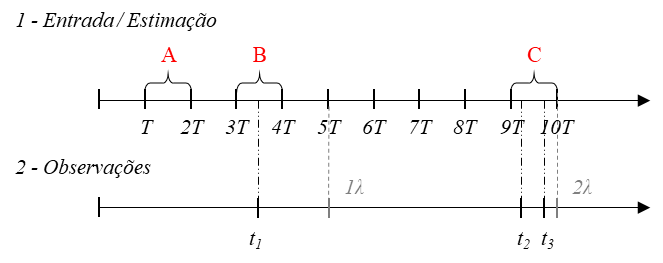
\includegraphics[scale=0.65]{Imagens/esquema2}
	\caption[Exemplos de instantes de amostragem da entrada e das estima��es]{Exemplos de instantes de amostragem da entrada e das estima��es (1) e das observa��es (2). Os instantes m�ltiplos de $\lambda$, igual ao intervalo m�dio de amostragem das observa��es s�o apresentados em cinza escuro, para refer�ncia.}
	\label{fig:esquema}
\end{figure} 



\subsection{Input Irregular Sampling}

Em caso de amostragem irregular tamb�m na entrada, um esquem�tico dos instantes de estima��o, amostragem e entrada pode ser observado na Fig.~\ref{fig:esquema2}

\begin{figure}[!htb]
	\centering
	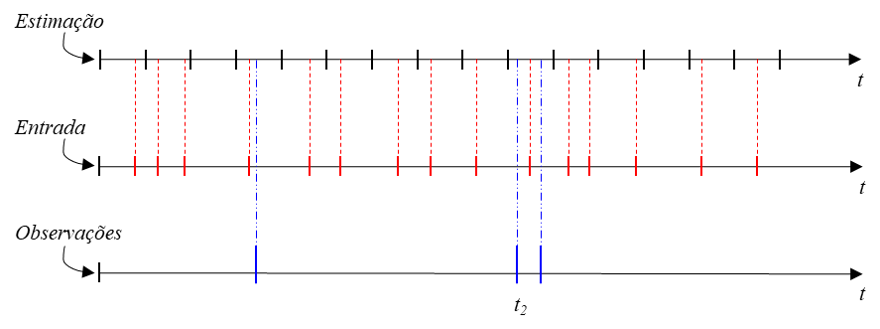
\includegraphics[scale=0.65]{Imagens/esquema3}
	\caption[Exemplos de instantes de amostragem de estima��o]{Exemplos de instantes de amostragem de estima��o(1), da entrada (2) e das observa��es (3). Os instantes m�ltiplos de $\lambda$, igual ao intervalo m�dio de amostragem das observa��es s�o apresentados em cinza escuro, para refer�ncia.}
	\label{fig:esquema2}
\end{figure} 

Para atrasos de transmiss�o:

\begin{figure}[!htb]
	\centering
	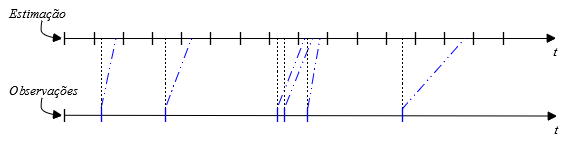
\includegraphics[scale=0.65]{Imagens/esquema4}
	\caption[Exemplos de instantes de amostragem de estima��o com atraso de tempo]{Exemplos de instantes de amostragem de estima��o(1), da entrada (2) e das observa��es (3). Os instantes m�ltiplos de $\lambda$, igual ao intervalo m�dio de amostragem das observa��es s�o apresentados em cinza escuro, para refer�ncia.}
	\label{fig:esquema3}
\end{figure} 

Nas pr�ximas subse��es � apresentado como os algoritmos de estima��o tratam os cen�rios \textbf{A}, \textbf{B} e \textbf{C} para os casos em que o carimbo de tempo est� e n�o est� dispon�vel.


\section{With Timestamp}\label{sec:carimbo}

Sabendo o momento exato $t_k$ em que as observa��es s�o medidas, � poss�vel assimil�-las no instante correto, considerando intervalos de tempo vari�veis para o algoritmo de filtragem. Para isso, o modelo matem�tico em () � discretizado a uma taxa $\delta t^*_j$ vari�vel. Para a simula��o deste artigo, os valores de $\delta t^*_j$ s�o calculados a partir da uni�o de todos os instantes de tempo correspondentes �s chegadas de sinais de entrada ou de medi��o em um �nico vetor, de forma ordenada. Por meio da subtra��o de dois instantes consecutivos, � poss�vel obter os intervalos de tempo de integra��o $\delta t^*_j$ correspondente. No caso de uma vers�o \textit{online}, a integra��o das equa��es diferenciais � executada a medida que um sinal de entrada ou um sinal de medi��o de sa�da � recebido. Nesses momentos, s�o utilizados o intervalo de tempo entre o �ltimo sinal recebido e o instante atual. Al�m disso, quando o sinal recebido � um sinal de entrada, � executada apenas a etapa de predi��o. E, quando o sinal for de medi��o, acontecem as duas etapas de predi��o e assimila��o de dados, considerado um segurador de ordem zero para a entrada. O fluxograma da Fig.~\ref{fig:diagrama} representa o passo a passo desse algoritmo, apresentando as etapas executadas quando o sinal � de entrada ou de observa��o.

Dessa forma, no cen�rio \textbf{B} da Fig.~\ref{fig:esquema}, o algoritmo executa uma etapa completa de predi��o e assimila��o de dados dos instantes $3T$ at� $t_1$, considerando o intervalo $\delta t^*_4 =t_1-3T$ (note que h� 3 intervalos de tempo $\delta t^*_j$, antes o instante $t_1$). Em seguida � feita uma etapa de predi��o entre $t_1$ e $4T$. Durante o intervalo de tempo de integra��o entre $t_1$ e $4T$, considerou-se que a entrada permaneceu constante desde a sua �ltima atualiza��o em 3T. Ou seja, assume-se que n�o houve varia��o na entrada para essa etapa de predi��o. Caso mais de uma observa��o seja medida entre duas entradas (cen�rio \textbf{C}), s�o executadas etapas completas de filtragem para cada observa��o dispon�vel e, ao final, uma etapa de predi��o entre a �ltima observa��o e a pr�xima entrada.

\section{Without Timestamp}

Quando o carimbo de tempo est� dispon�vel, a assimila��o de dados do algoritmo pode ser feita nos momentos exatos da medi��o. Para isso, a integra��o das equa��es diferenciais via discretiza��o deve acontecer com intervalos de tempo vari�veis, no caso deste trabalho utilizando o m�todo de Runge-Kutta de 4� ordem. Dessa forma, (\ref{eq:processo}) pode ser reescrita como
\\
\begin{equation}\label{eq:disc_carimbo}
x(t^*_j)=f_\textrm{d}(x(t^*_{j-1}),u(t^*_{j-1}),w(t^*_{j-1}),t^*_{j-1}),
\end{equation}
\\
\noindent
em que $t^*_j= t^*_{j-1} + \delta t^*_j$ e $t^*_0=0$. Cada valor $\delta t^*_j$ corresponde ao intervalo de tempo entre o �ltimo instante $t^*_{j-1}$ em que se registrou a chegada de um sinal, seja ele de entrada ou de observa��o, e o pr�ximo instante de tempo $t^*_{j}$ em que um valor de entrada ou de observa��o � obtido, conforme ser� detalhado no Cap�tulo \ref{cap3}. Entre instantes de observa��o e de entrada � utilizado um segurador de ordem zero, considerando a ultima informa��o dispon�vel. 

Por outro lado, se o carimbo de tempo n�o � levado em conta, (\ref{eq:processo}) pode ser reescrito como

\begin{equation}\label{eq:disc_semcarimbo}
x_n=f^*_\textrm{d}(x_{n-1},u_{n-1},w_{n-1},n),
\end{equation}
\\
\noindent
em que $t=nT$.


Quando n�o h� carimbo de tempo nas medi��es, o algoritmo de filtragem n�o sabe o momento exato da medi��o $t_k$. Assim, o instante de tempo considerado para a etapa de assimila��o de dados � sempre o pr�ximo instante m�ltiplo de \textit{T}, i.e. quando a pr�xima informa��o de entrada est� dispon�vel.
%
Existem apenas dois cen�rios de estima��o nesse caso. Primeiro, quando n�o h� medi��es dispon�veis entre duas entradas, o estimador executa apenas a etapa de predi��o entre os intervalos de tempo $iT$ e $(i+1)T$, conforme cen�rio \textbf{A} da Fig.~\ref{fig:esquema}. Segundo, nos casos representados pela letra \textbf{B}, o estimador considera que a observa��o foi feita no pr�ximo instante multiplo de $T$ em que h� informa��es de entrada. No exemplo da Fig.~\ref{fig:esquema}, a medi��o feita no instante $t_1$ � assimilada no instante $4T$. Caso haja mais de uma observa��o entre duas entradas (cen�rio \textbf{C}), a mais antiga � descartada. Os passos de discretiza��o do modelo utilizados pelo UKF s�o sempre $\delta t=T$, havendo ou n�o observa��es dispon�veis. 

\vspace{0.5cm}
\begin{figure}
	\centering
	\begin{adjustbox}{width=\textwidth/2,height=\textheight,keepaspectratio}
		
		\begin{tikzpicture}[node distance=2cm, font = \scriptsize]
		
		\node(start)[startstop][text width=3cm,align=center]{\textbf{In�cio} \\ $t^*_0=0$; \\ $i=j=k=1$; \\};
		
		\node (dec1) [decision, below of=start,yshift=-0.5cm] {Sinal Recebido};
		
		\node (pro1) [process, below right of=dec1, yshift=-0.7cm, xshift=0.25cm][text width=3cm,align=center]{Calcula \\ $\delta t^*_{j} = iT - t^*_{j-1}$ \\ $t^*_{j} = t^*_{j-1} + \delta t^*_{j}$};
		
		\node (pro12) [process, below of=pro1][text width=3cm,align=center, yshift=0.5cm]{Etapa de Predi��o};
		
		\node (pro2) [process, below left of=dec1,  yshift=-0.7cm, xshift=-0.25cm][text width=3cm,align=center]{Calcula \\ $\delta t^*_{j} = t_k - t^*_{j-1}$ \\ $t^*_{j} = t^*_{j-1} + \delta t^*_{j}$};
		
		\node (pro22) [process, below of=pro2][text width=3cm,align=center, yshift=0.5cm]{Etapa de Predi��o, utilizando ZOH};
		
		\node (pro23) [process, below of=pro22][text width=3cm,align=center, yshift=0.5cm]{Etapa de Assimila��o de Dados};
		
		\node (pro3) [startstop, below of = pro23][text width=3cm,align=center, xshift=1.8cm]{Estimativa em $t^*_{j}$};
		
		\draw [arrow] (start) -- node[pos=0.5](h){} (dec1);
		\draw [arrow] (dec1) -| node[text width=3cm,align=center,anchor=west,xshift=-1cm] {Sinal de \\ Entrada} (pro1);
		\draw [arrow] (dec1) -| node[text width=3cm,align=center,anchor=east,xshift=0.8cm] {Sinal de \\ Observa��o} (pro2);
		\draw [arrow] (pro1) -- (pro12);
		\draw [arrow] (pro2) -- (pro22);
		\draw [arrow] (pro22) -- (pro23);
		\draw [arrow] (pro12) -- node[text width=3cm,align=center,anchor=south,xshift=1cm] {$i=i+1$} (pro3);
		\draw [arrow] (pro23) -- node[text width=3cm,align=center,anchor=east,xshift=0.6cm] {$k=k+1$}(pro3);
		\draw [arrow] (pro3) --+(-4cm,0) |- node[text width=3cm,align=center,anchor=south,xshift=1cm] {$j=j+1$}(h);
		\end{tikzpicture}
	\end{adjustbox}
	
	\caption[Diagrama ilustrativo da vers�o \textit{online} do estimador]{Diagrama ilustrativo da vers�o \textit{online} do estimador que considera o carimbo de tempo. Os �ndices $i$, $j$ e $k$ representam, respectivamente os contadores dos sinais de entrada, estima��o e da sa�da.}
	\label{fig:diagrama}
\end{figure}	





\clearpage

\clearpage
\thispagestyle{empty}
\cleardoublepage
%
%%%%--------------------------------------------------------------------
%Cap�tulo 5 - Conclusions
%-------------------------------------------------------------------------------
\chapter{Results}
\label{cap4} \vspace{-1cm} \vspace{1cm}

%\begin{flushright}
%\begin{minipage}{0.7\linewidth}
%\emph{``O homem � como uma fun��o, cujo numerador � o que ele � e
%cujo denominador � o que ele pensa dele mesmo. Quanto maior o
%denominador, menor a fra��o.''}
%\end{minipage}
%\end{flushright}
%
%\begin{flushright}
%{L. N. Tolst�i}
%\end{flushright}

%\section{Introdu��o}

In this chapter, we present simulation results for two different systems: a linear system with two under damped modes and a nonholomonic unicycle position system.

REVISAR

\textit{We begin by describing the simulated systems as a state-space representation. First system is discretized and a discrete Kalman filter is used for the estimation of the unicycle position. The second one is represented as a continuous-time process model with digital measurements of one stby aate. We wish to estimated a all states  sampled-data Kalman filter.}

For both cases, we start evaluating the effect of time-stamp information in the estimation algorithm for three different irregular sampling scenarios, without time-delay in the observations: variation of the observation signal-to-noise ratio, variation of the observation average sampling rate, and variation of the relation between estimation regular sampling rate and output irregular average sampling rate. 

Then we add random time-delay to the observation model and evaluate the effect for the same three scenarios plus a fourth one, where we vary the average time-delay.


\section{Linear System}

\textit{Descrever as motiva��es por tr�s do estudo do sistema linear: vari�veis controladas, resultado esperado conhecido, compara��o mais clara.}


\subsection{System Description}

The linear system designed for simulation is the serial combination of two under damped modes, with distinct band pass behaviors.

One of the modes, henceforth termed as low-pass (lp) system, has time constant $\tau_{lp} = 1$ s, natural frequency $\omega_{n,lp} = 10$ Hz and a damping constant of $\zeta_{lp}=0.1$. The frequency response is given by:

\begin{equation}\label{eq:aircraft}
G_{lp}(s) = \frac{100}{s^2 + 2s + 100}\\
\end{equation}


The second mode is a high-pass (hp) system, with a much lower time constant $\tau_{hp} = 0.01$ s, natural frequency $\omega_{n,hp} = 1000$ Hz, same damping constant of $\zeta_{hp}=0.1$ and two zeros, one at the origin and another one at $0.001$. The high-pass frequency response is given by:

\begin{equation}\label{eq:aircraft}
G_{hp}(s) = \frac{s^2-0.001s}{s^2 + 200s + 10^6}\\
\end{equation}

Figure~\ref{fig:bode} shows the bode diagrams of both systems separately.

%\begin{figure}[!htb]
%	\centering
%	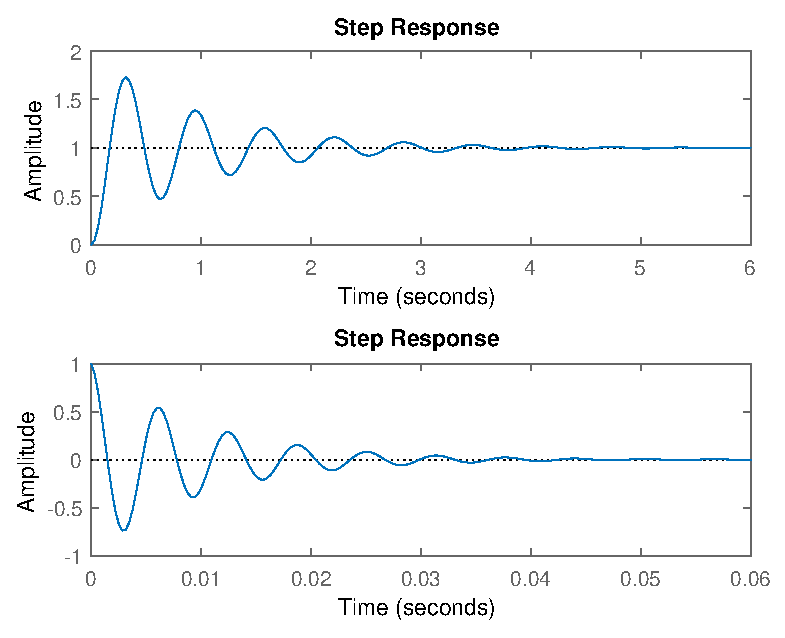
\includegraphics[width=0.6\textwidth]{Imagens/stepResponse.eps}
%	\caption[entrada]{Step response of both low-pass and high-pass modes.}
%	\label{fig:stepResponse}
%\end{figure}

\begin{figure}[!htb]
	\centering
	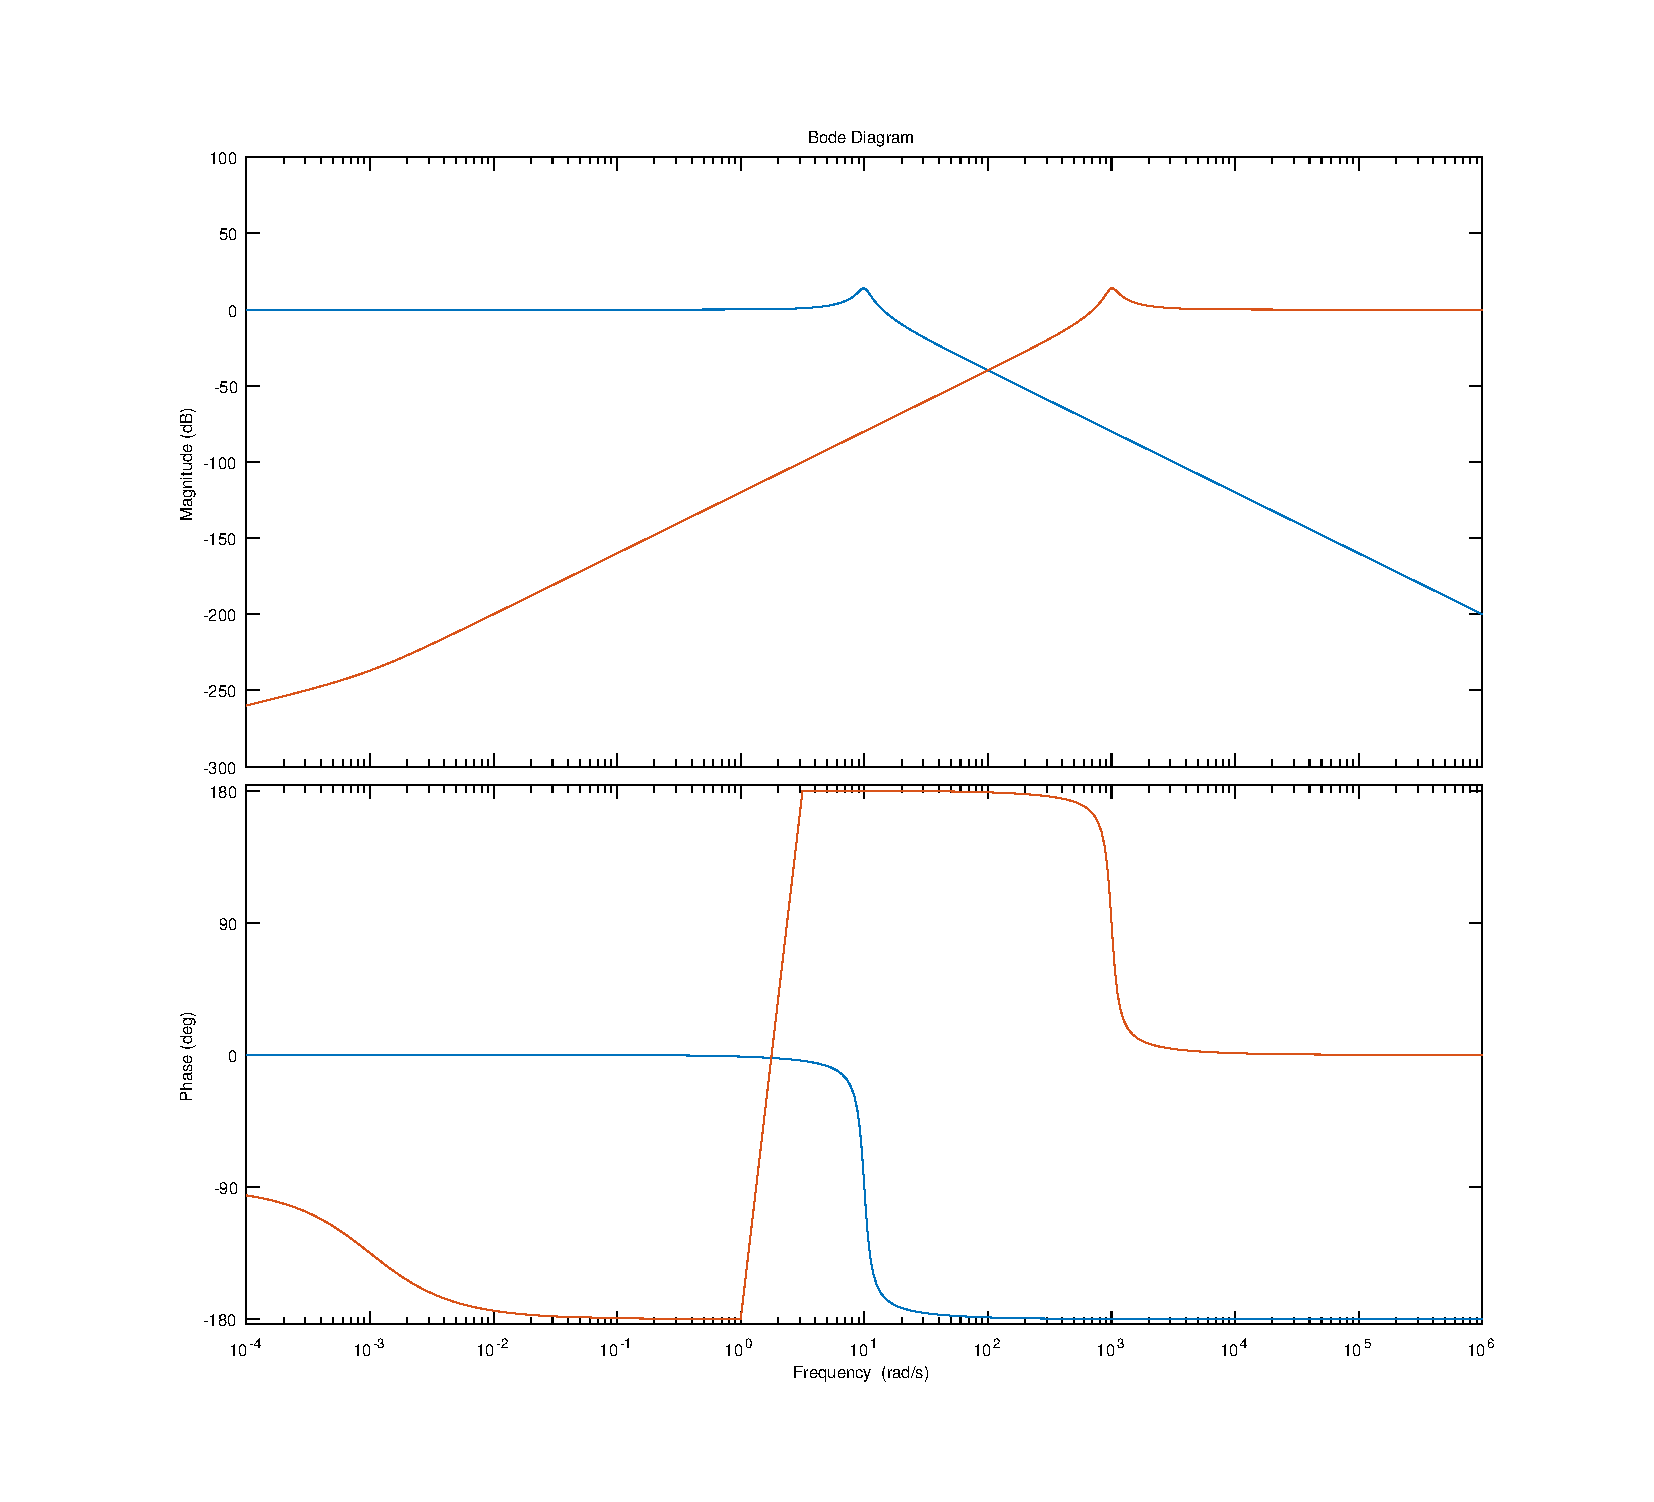
\includegraphics[width=0.6\textwidth]{Imagens/bode.eps}
	\caption[entrada]{Bode diagram of both modes.}
	\label{fig:bode}
\end{figure}

%\begin{figure}[!htb]
%	\centering
%	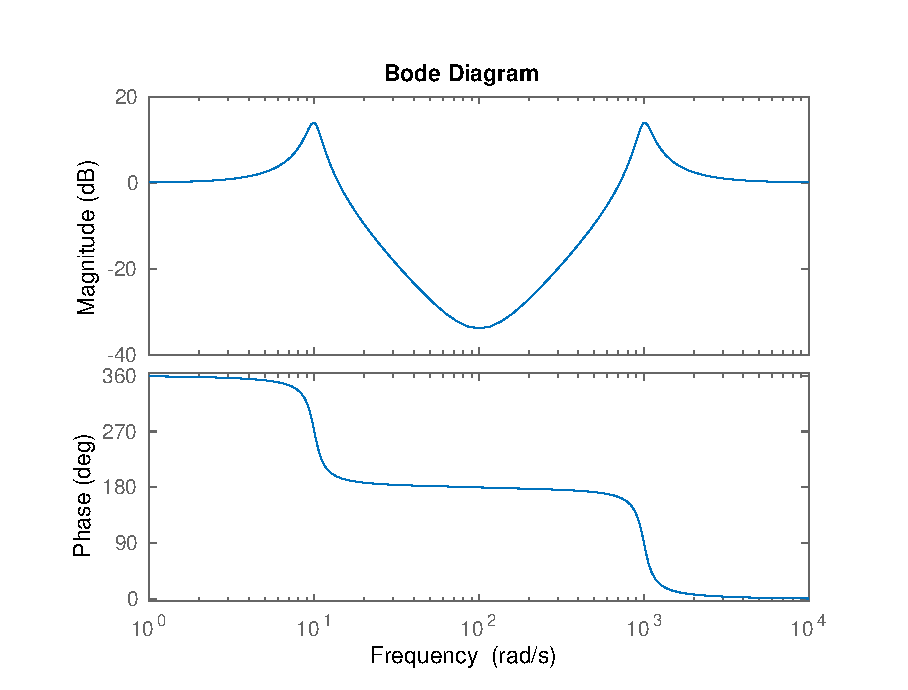
\includegraphics[width=0.6\textwidth]{Imagens/bodeS.eps}
%	\caption[entrada]{Bode diagram of the resulting fourth order system.}
%	\label{fig:bodeS}
%\end{figure}


The resulting fourth order system is described as a state space representation, in a modal canonical form given by:

\begin{equation}
\begin{split}
\dot{x}(t) & = Ax(t) + Bu(t) \\
y(t) & = Cx(t) + Du(t)
\end{split}
\end{equation}


\noindent
where $x(t) \in \mathbf{R}^4$ is the state vector, $u(t) \in \mathbf{R}^1$ is the single input vector and $y(t) \in \mathbf{R}^1$ is the single output vector, and

\begin{equation}
\begin{split}
A & =\begin{bmatrix}
-100 & 994.99 & 0 & 0\\
-994.99 & -100 & 0 & 0\\
0 & 0 & -1 & 9.949\\
0 & 0 & -9.949 & -1
\end{bmatrix} \\
\\
B & =\begin{bmatrix}
-24.6435 \\
-18.8943 \\
-4.1746 \\
-0.2675
\end{bmatrix} \\
\\
C & =\begin{bmatrix}
24.41 & -21.2522 & -0.1537 & 2.3977 \\
\end{bmatrix} \\
\\
D & =1
\end{split}
\end{equation}

%
%\begin{equation}\label{eq:sistemaLinear}
%\begin{split}
%Z_{de} & := (\partial Z/\partial \delta_e)/m = -61.655 \ m/s^2,\\
%Z_q & := (\partial Z/\partial q)/m = -5.132 \ m/s,\\
%Z_w & := (\partial Z/\partial W)/m = -3.1332 \ s^{-1},\\
%M_{de} & := (\partial M/\partial \delta_e)/I_y = -40.465 \ s^{-2},\\
%M_q & := (\partial M/\partial q)/I_y = -2.6864 \ s^{-1},\\
%M_w & := (\partial M/\partial W)/I_y = -0.04688 \ (s-m)^{-1},\\
%\tau & = 0.1 \ s \\
%U_o & = 306.42 \ m/s
%\end{split}
%\end{equation}

We simulate a pseudo-random binary sequence (PRBS) as input, with 200 samples and simulate the high-pass and low-pass systems separately according to Figure~\ref{fig:PRBS_and_systems}. As expected, the low-pass response is much slower. Just for comparison, if the same 200 samples of PRBS was generated over 20 seconds, the low-pass system response would account for more variations in the input. Figure~\ref{fig:outputS} show the response of the final fourth order system.
\begin{figure}[!htb]
	\centering
	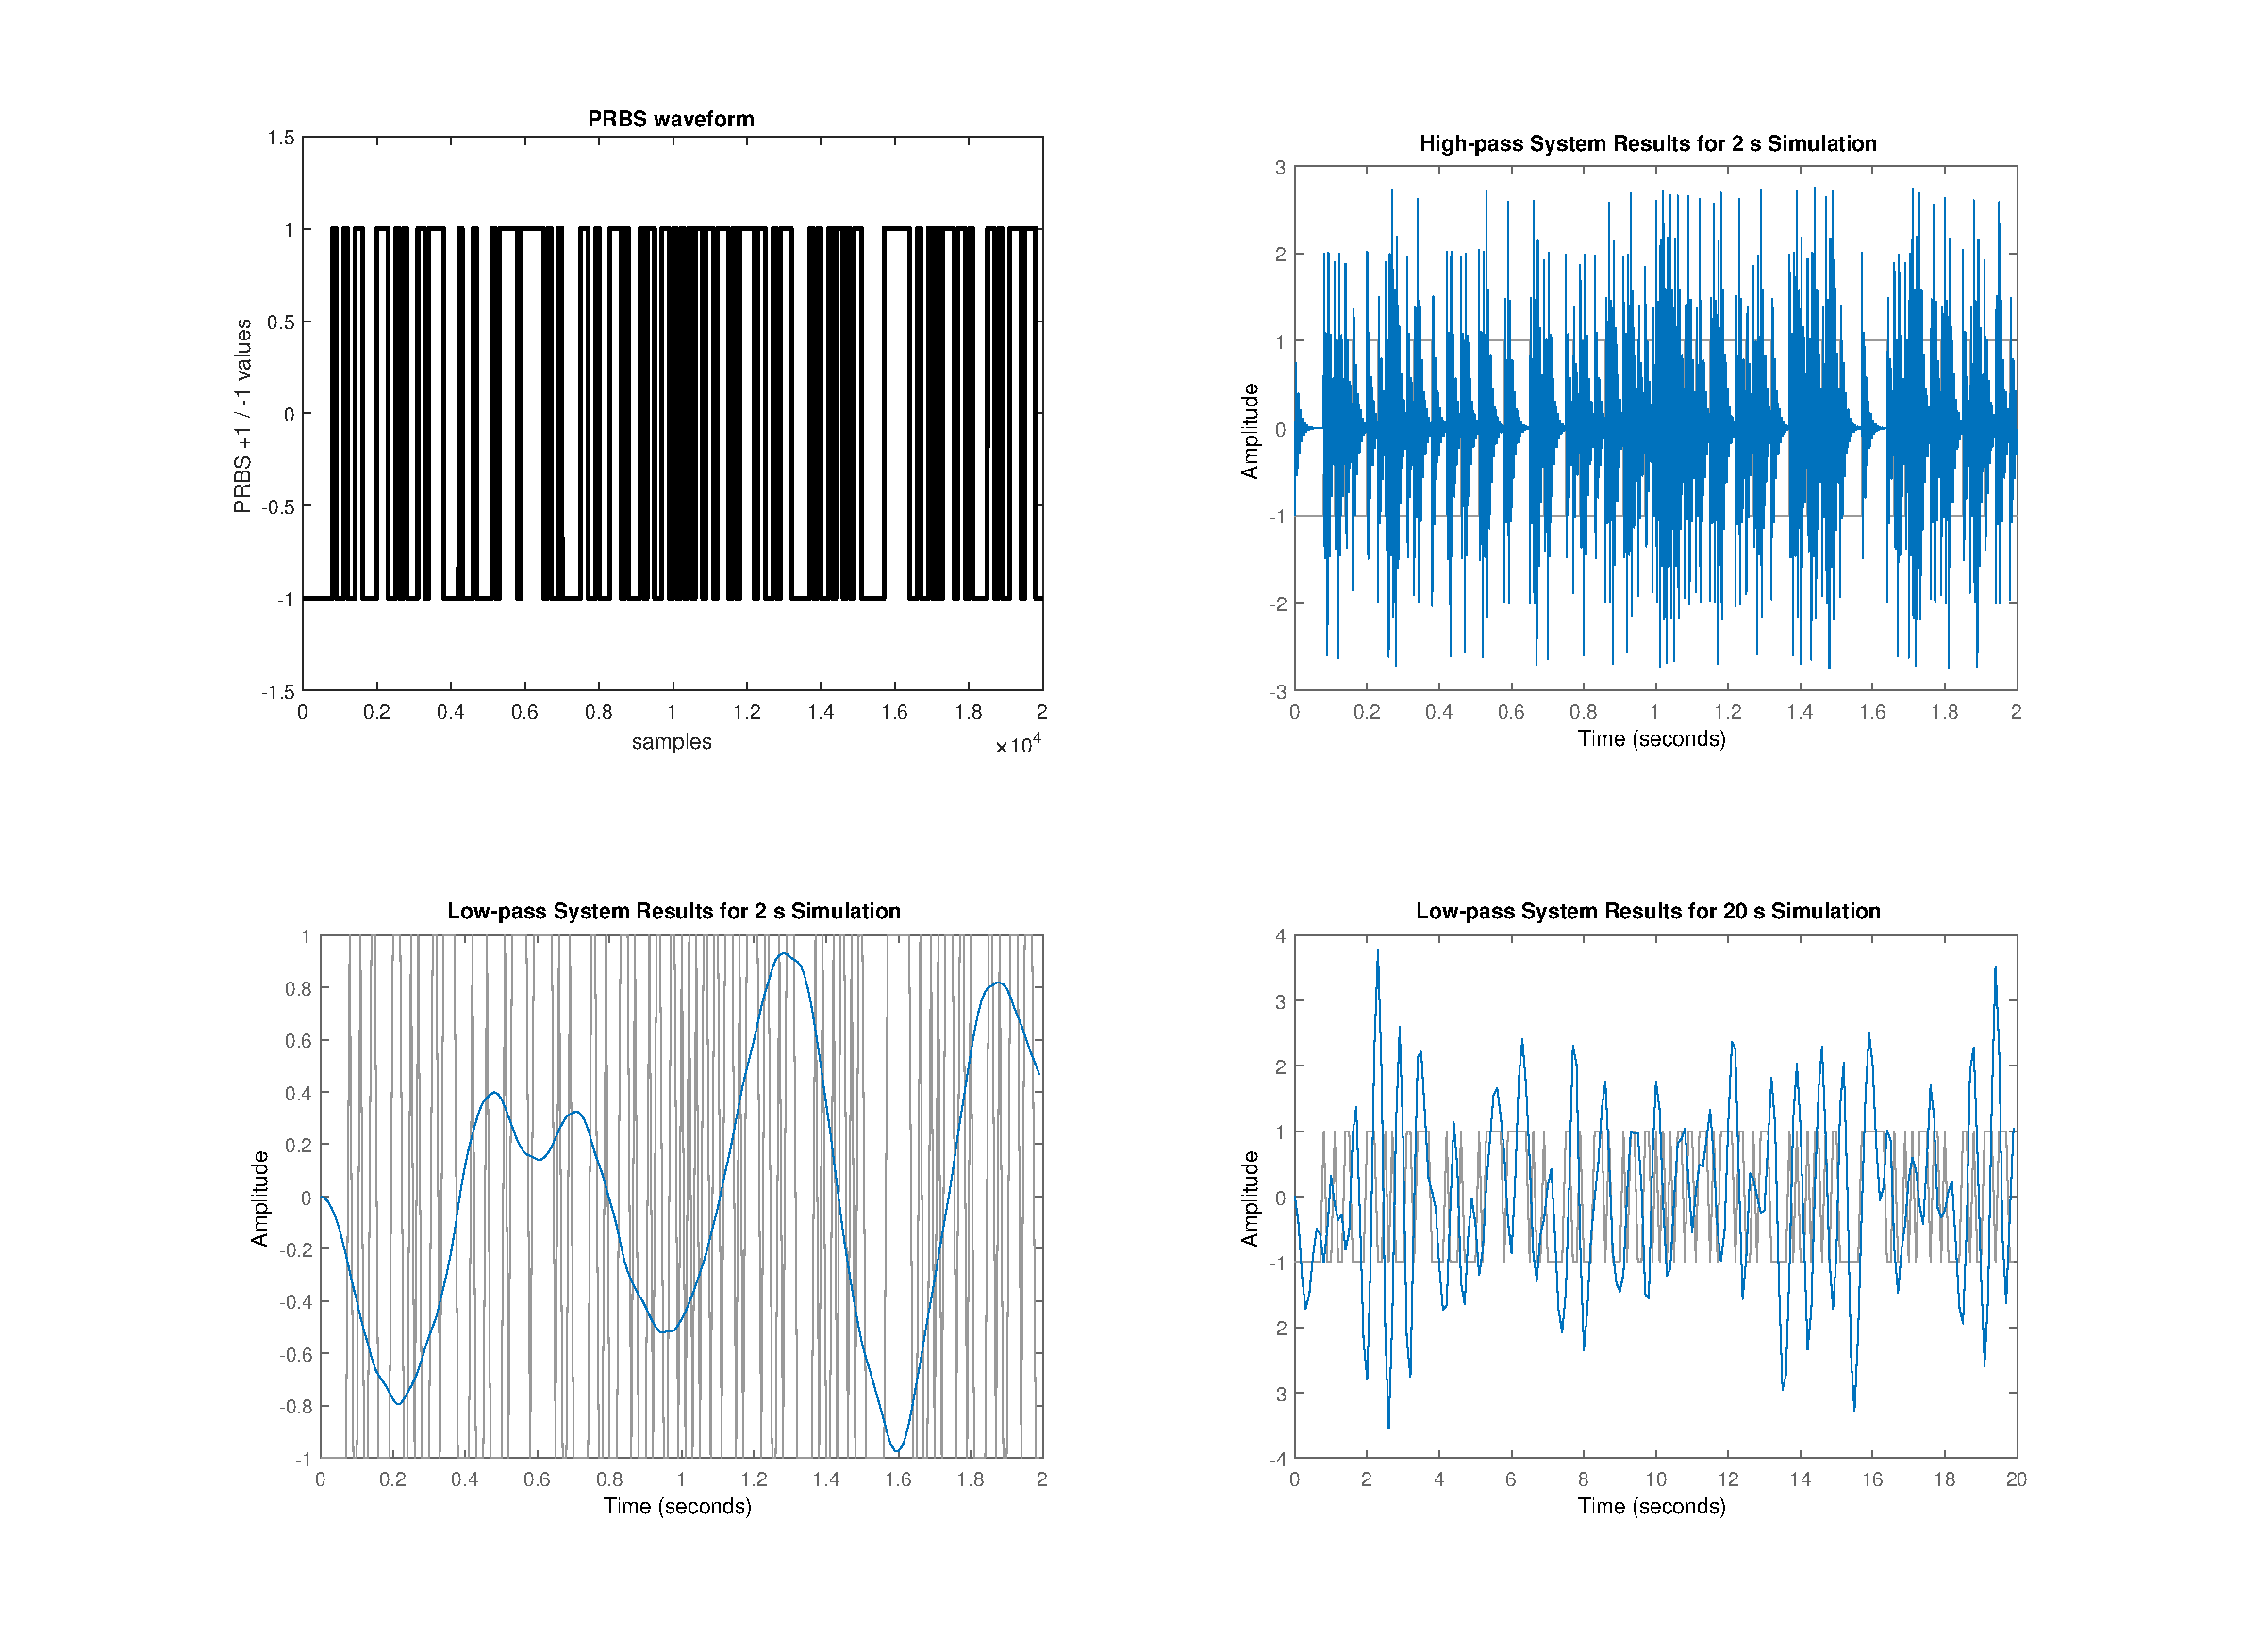
\includegraphics[width=\textwidth]{Imagens/PRBS_and_Systems.eps}
	\caption[entrada]{PRBS samples used as input; output of high-pass system, considering 2 seconds of simulation and low-pass system results for 2 and 20 seconds simulation}
	\label{fig:PRBS_and_systems}
\end{figure}

%\begin{figure}[!htb]
%	\centering
%%	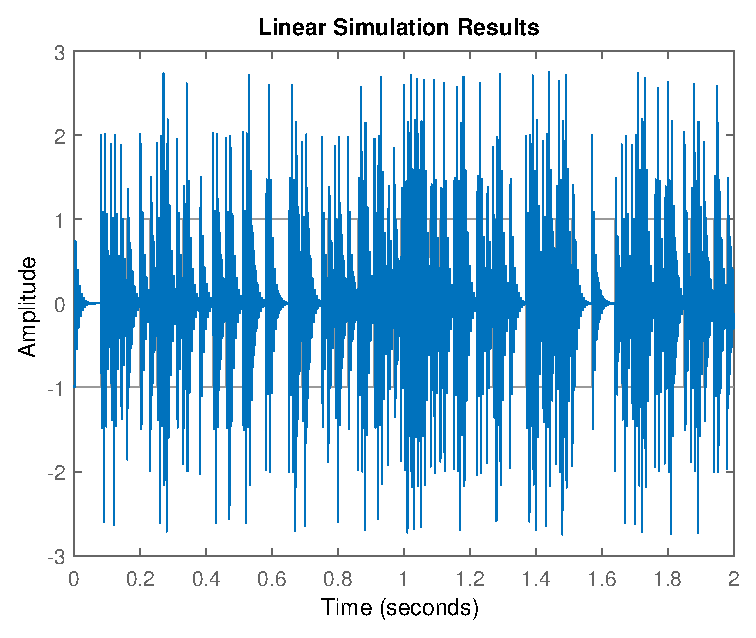
\includegraphics[width=0.6\textwidth]{Imagens/outputS2.eps}
%	\caption[entrada]{Output of high-pass system to the PRBS input signal}
%	\label{fig:outputS2}
%\end{figure}
%
%As expected, the low-pass response is much slower. Just for comparison, if the same 200 samples of PRBS was generated over 20 seconds, the low-pass system response would account for more variations in the input, as shown in Figure~\ref{fig:outputS1_2}
%
%\begin{figure}[!htb]
%	\centering
%	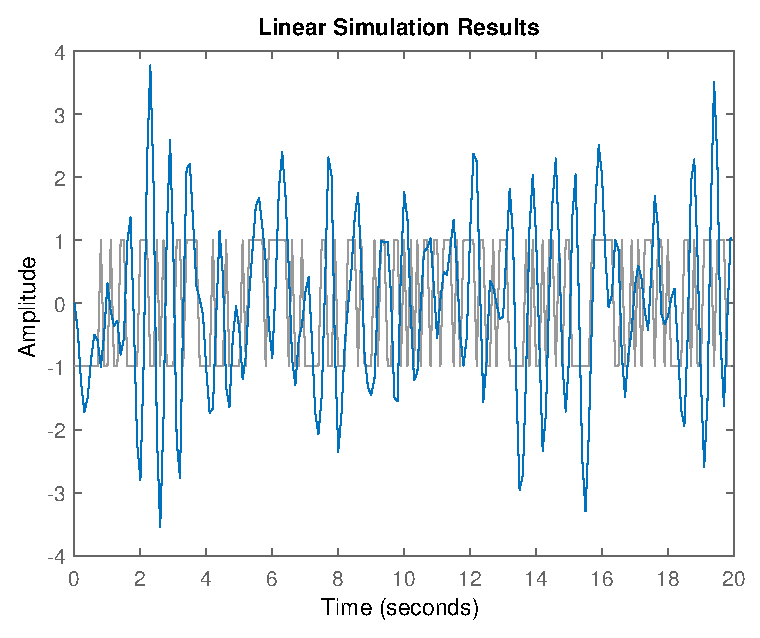
\includegraphics[width=0.6\textwidth]{Imagens/outputS1_2.eps}
%	\caption[entrada]{Output of low-pass system to the PRBS input signal extended over 20 seconds}
%	\label{fig:outputS1_2}
%\end{figure}
%
%The response of the final fourth order system, considering both modes is presented in Figure~\ref{fig:outputS}, where both modes dynamics can be observed.
%
\begin{figure}[!htb]
	\centering
	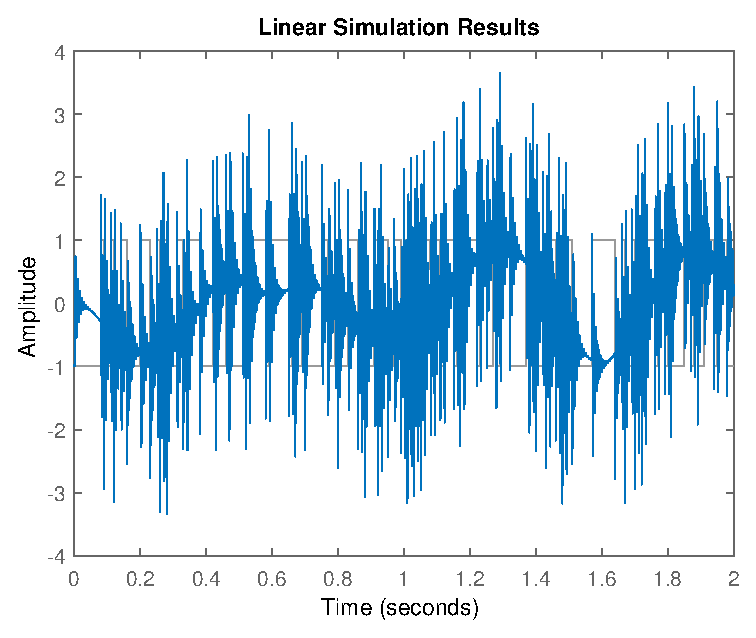
\includegraphics[width=0.5\textwidth]{Imagens/outputS.eps}
	\caption[entrada]{Output of the fourth order system to the PRBS input signal}
	\label{fig:outputS}
\end{figure}

The linear system is discretized using MATLAB's `c2d`fic

The sampled-data observations are available according to:

\begin{equation}
y(t_k) = \textbf{B}_dx(t)+\textbf{D}_du(t) + v(t_k)
\end{equation}

\noindent
where $v(t_k) \sim \mathcal{N} (0,R_{t_k})$ is the observation noise, with zero mean and covariance $R_{t_k}$. When time-stamp is not available, the observation vector is approximated by $\tilde{y}_i \approx y(t_k)$, where $i$ is the index of the next time instant, multiple of $T$.

Discrete-time Kalman filter is used for estimation. Realizations of the estimated states and true values for both scenarios, with and without time-stamp, for a signal-to-noise ration in the observations of $40$ dB are shown in Figures~\ref{fig:StatesWithAndWithoutTimeStamp} 

\begin{figure}[!htb]
	\centering
	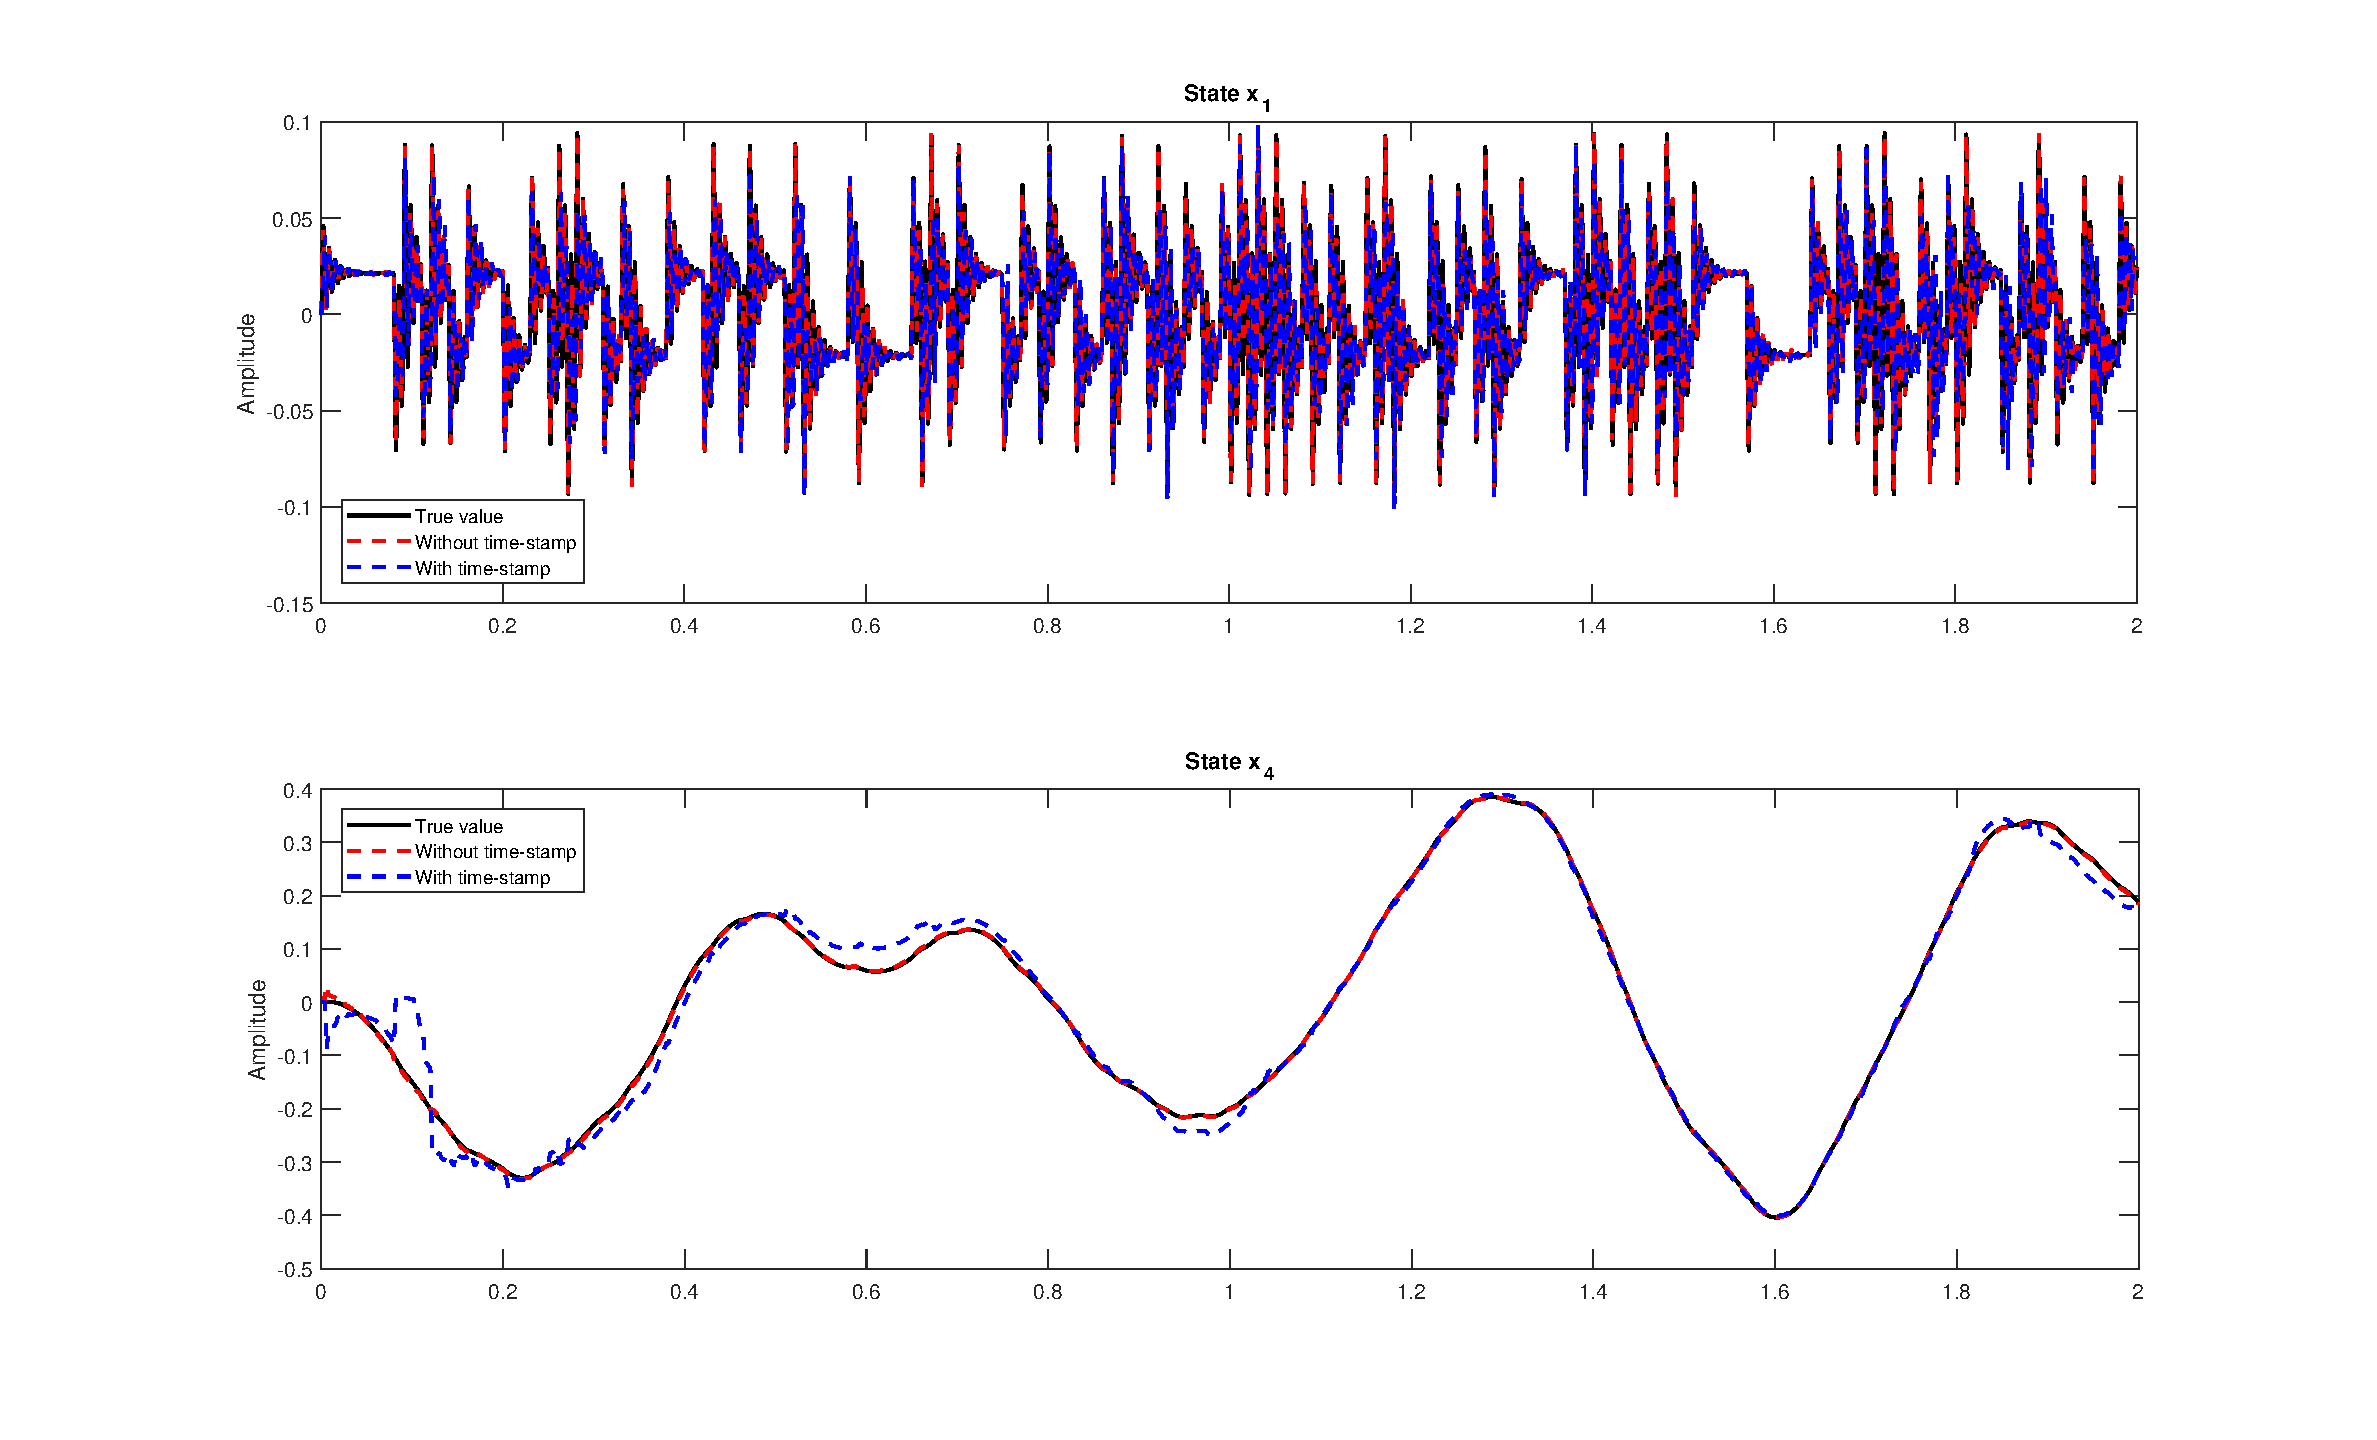
\includegraphics[width=\textwidth]{Imagens/StatesWithAndWithoutTimeStamp.eps}
	\caption[entrada]{Estimated with time-stamp (red), without time-stamp (blue) and true (black) states $x_1$ and $x_4$.}
	\label{fig:StatesWithAndWithoutTimeStamp}
\end{figure}

%\begin{figure}[H]
%	\centering
%	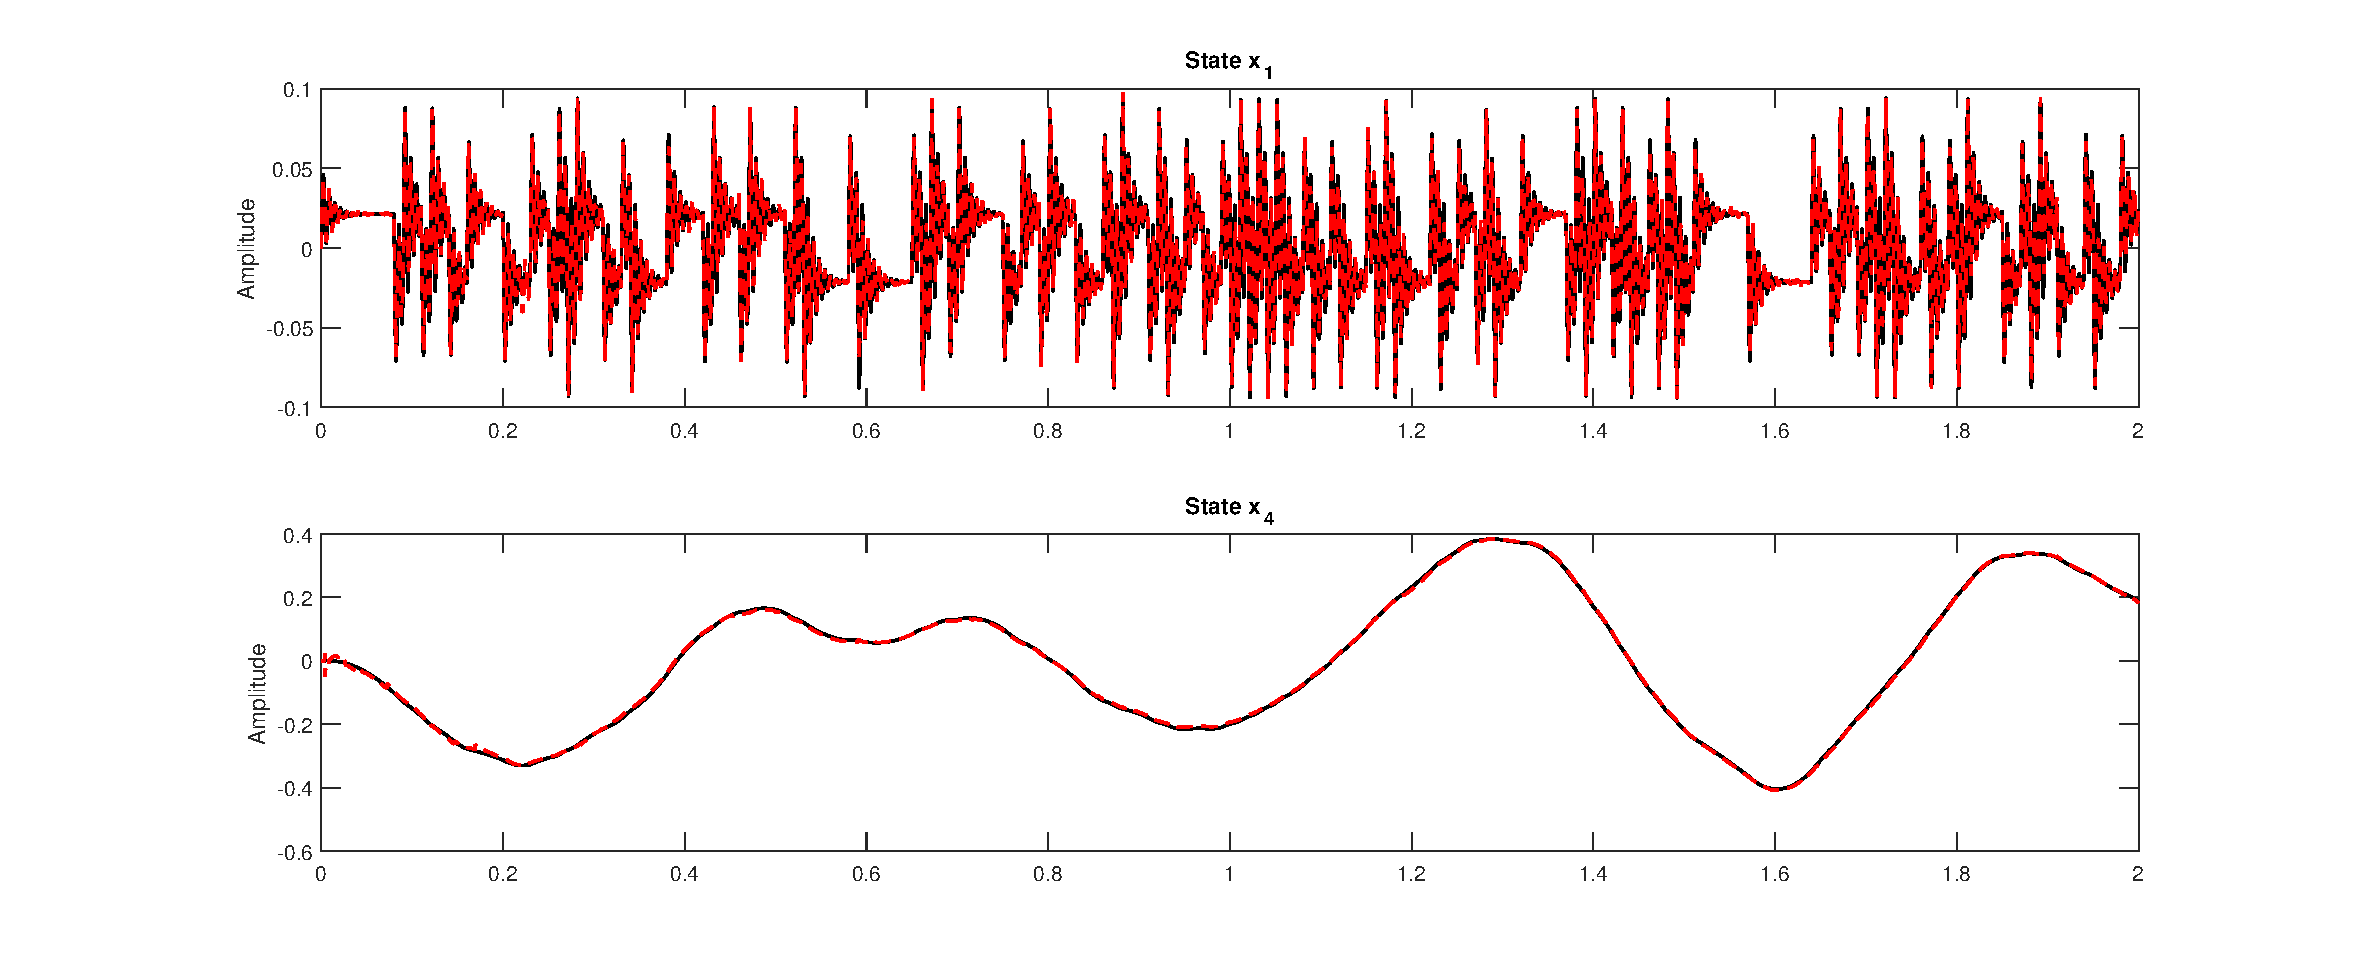
\includegraphics[width=\textwidth]{Imagens/StatesWithTimeStamp14.eps}
%	\caption[entrada]{Estimated (red) and true (black) states $x_1$ and $x_4$ considering time-stamp in the estimation algorithm.}
%	\label{fig:StatesWithTimeStamp}
%\end{figure}
%
%\begin{figure}[H]
%	\centering
%	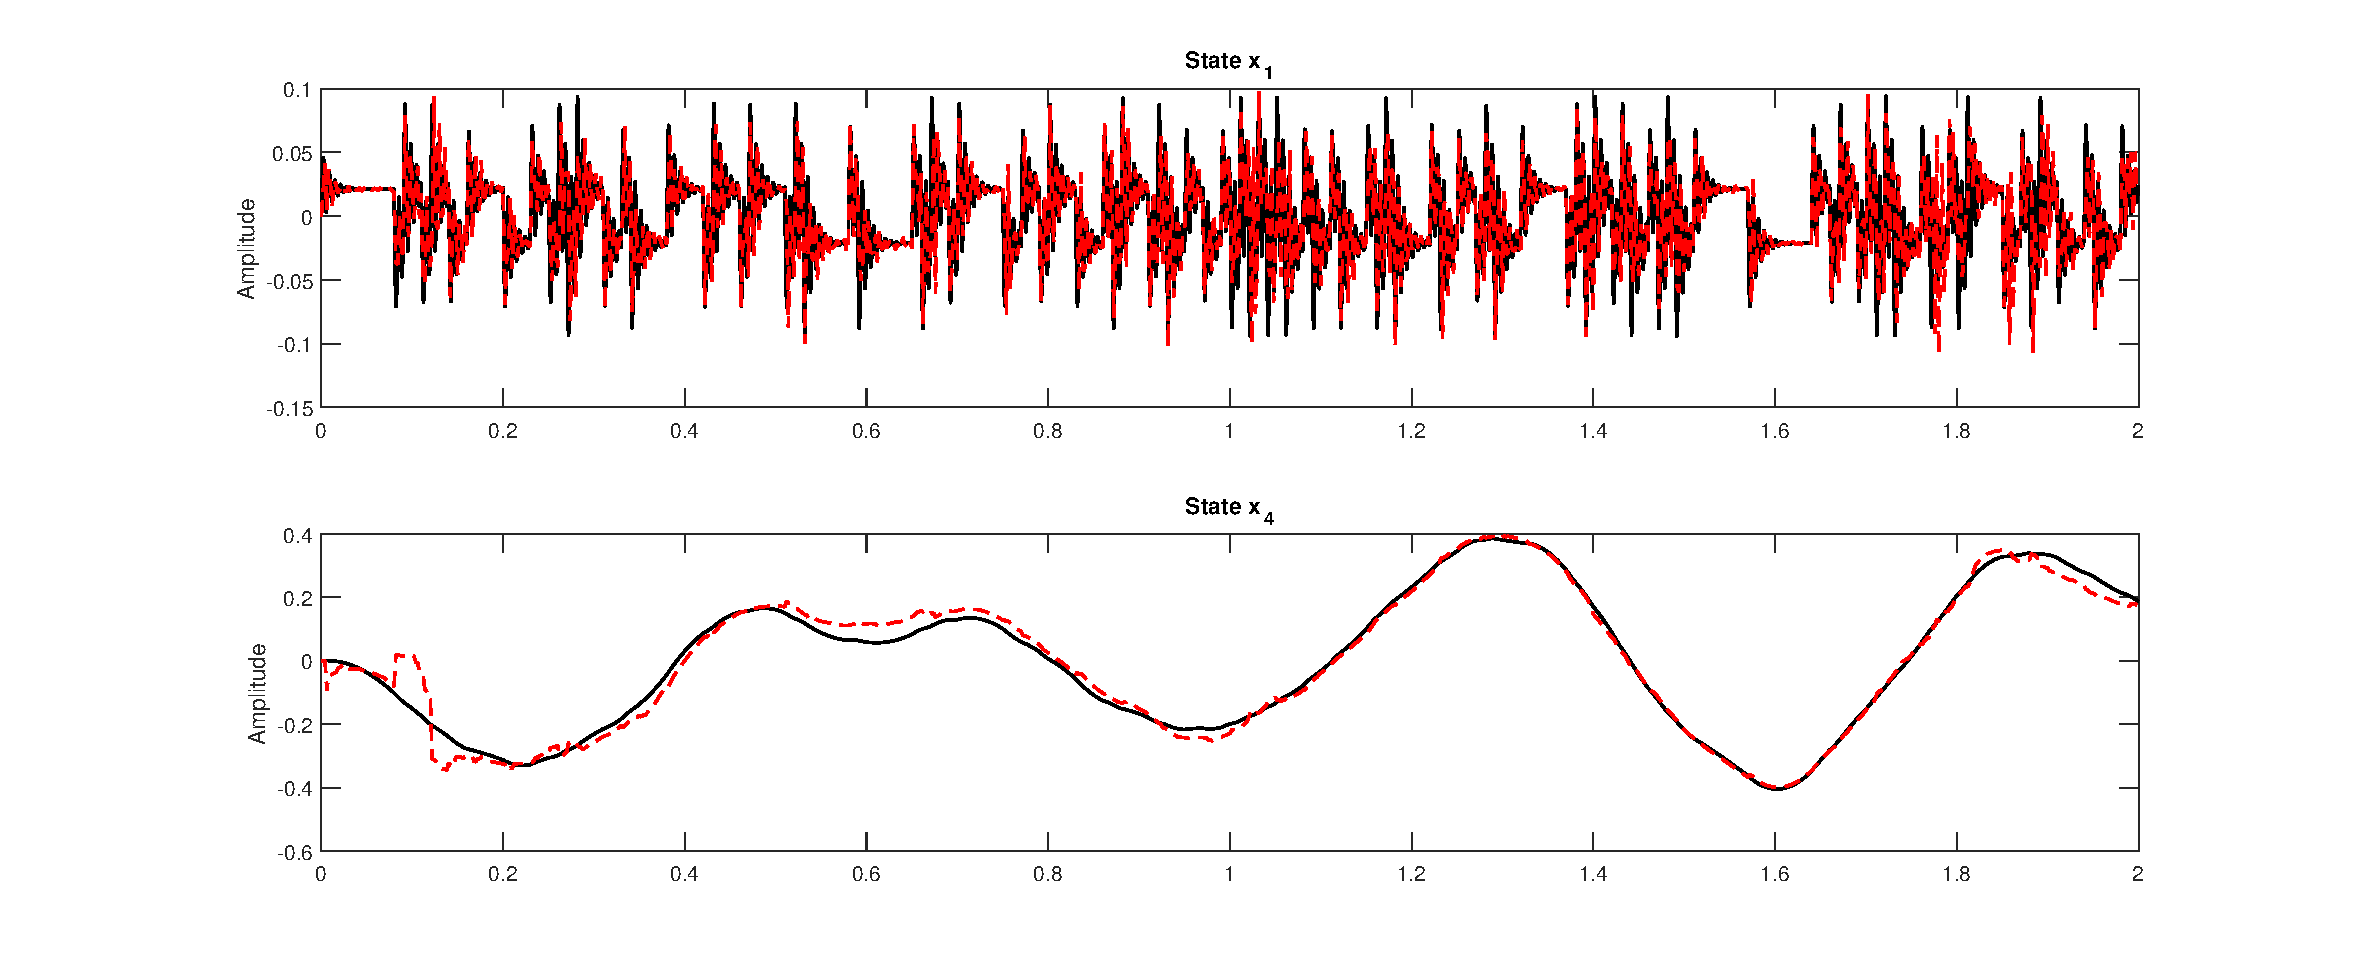
\includegraphics[width=\textwidth]{Imagens/StatesWithoutTimeStamp14.eps}
%	\caption[entrada]{Estimated (red) and true (black) states$x_1$ and $x_4$ not considering time-stamp in the estimation algorithm.}
%	\label{fig:StatesWithoutTimeStamp}
%\end{figure}

Figure~\ref{fig:LinearJevolution} presents a window data from 0 to 0.045 seconds of the first state RMSE for the algorithms with and without time-stamp. As expected, we observe a distancing from the RMSE at the instant the first observation was taken $t_1$, favoring the algorithm that considers time-stamp.

\begin{figure}[H]
	\centering
	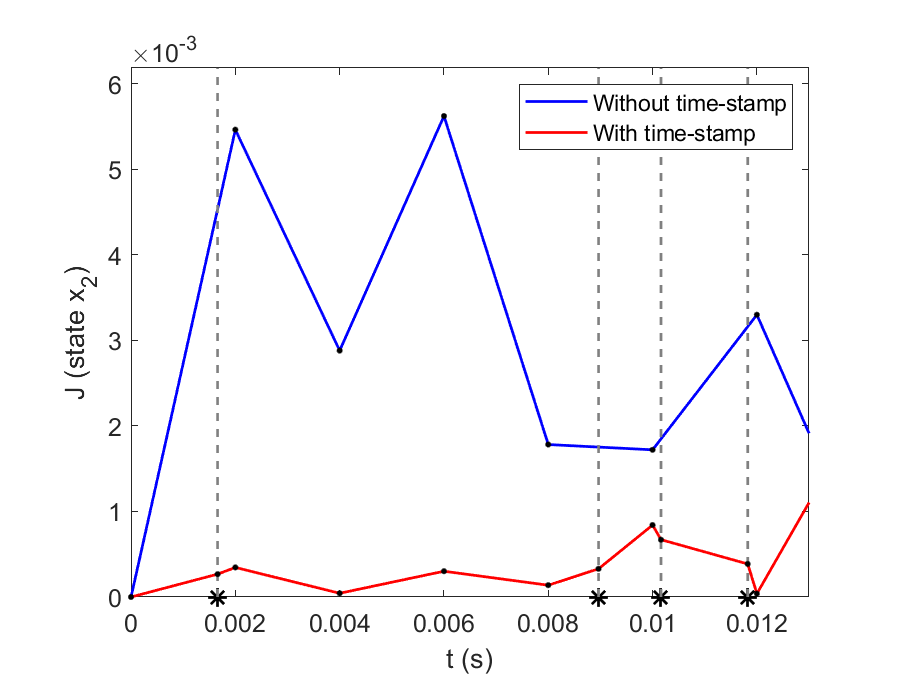
\includegraphics[width=0.6\textwidth]{Imagens/LinearJEvolution.eps}
	\caption[entrada]{Temporal cut from 0.02 to 0.045 seconds, for a realization of pitch rate about the center of mass RMSE of both estimators, with (\textcolor{red}{---}) and without (\textcolor{blue}{---}) time-stamp. Vertical dashed lines match the measurement sampling instants $t_k$. Black dots represent the regular estimation instants.}
	\label{fig:LinearJevolution}
\end{figure}



\begin{figure}[H]
	\centering
	{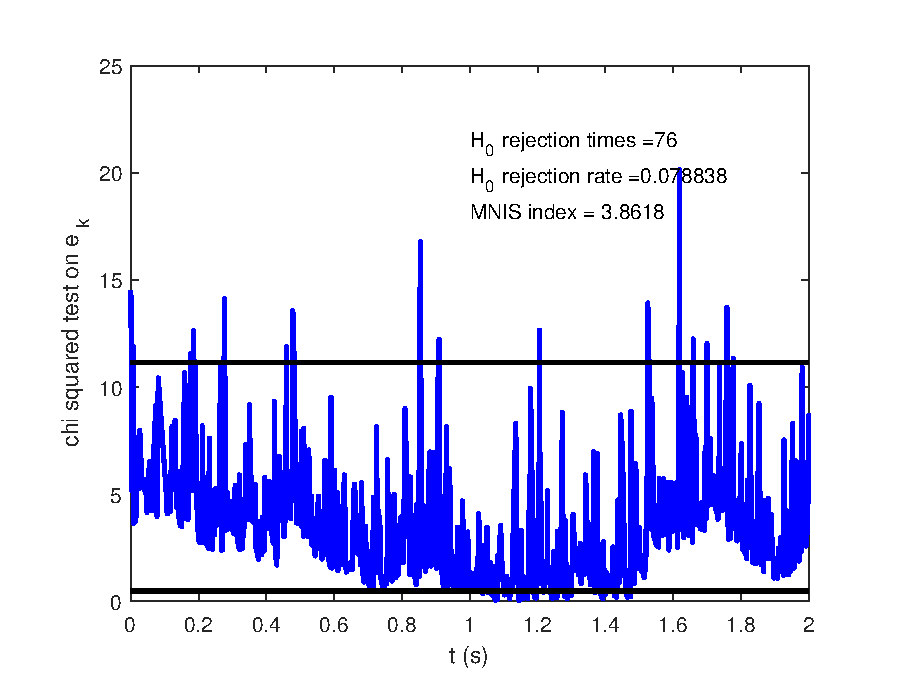
\includegraphics[width=.45\textwidth]{Imagens/chi_e_with.eps}}\quad
	{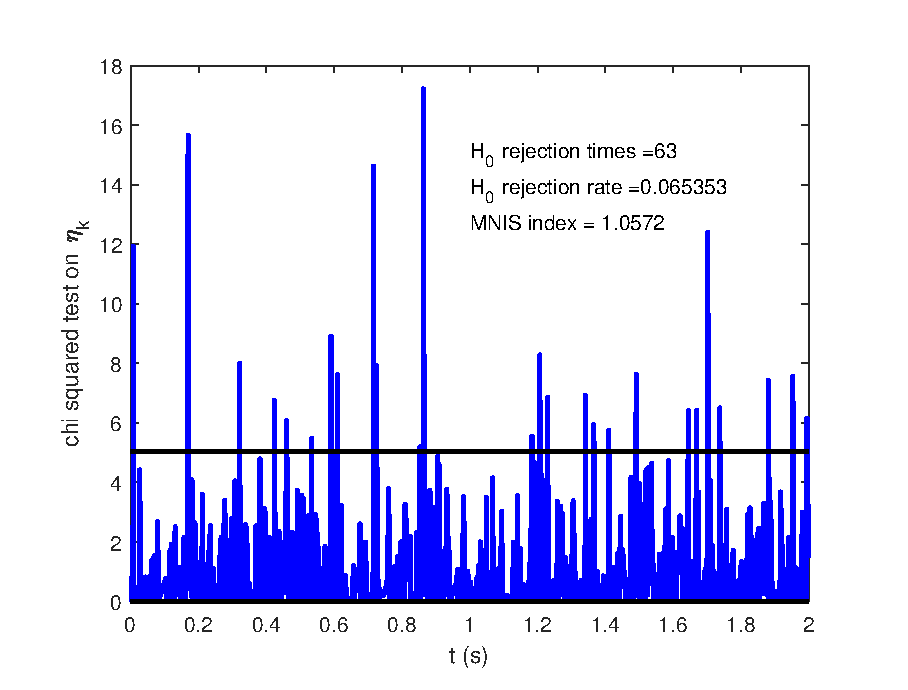
\includegraphics[width=.45\textwidth]{Imagens/chi_eta_with.eps}}\\
	{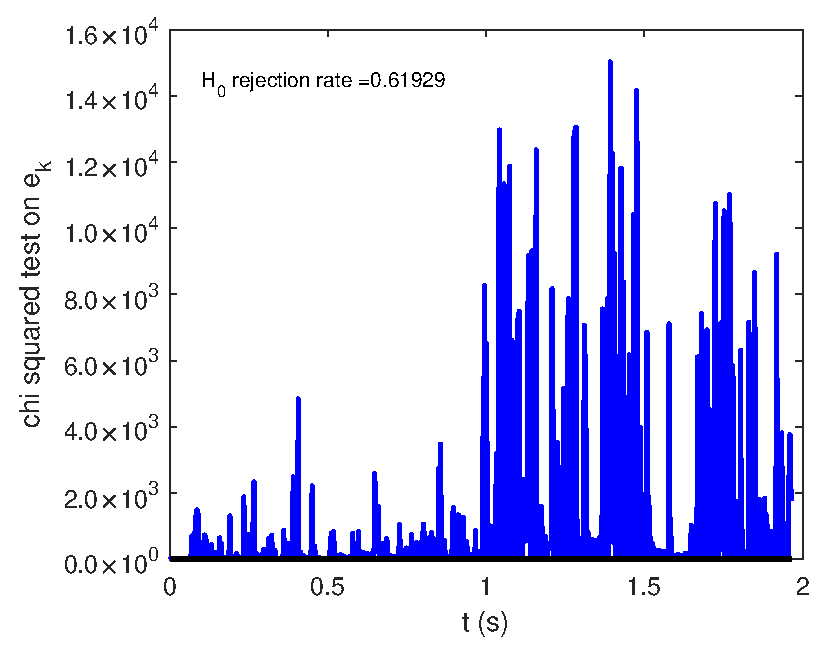
\includegraphics[width=.45\textwidth]{Imagens/chi_e_without.eps}}\quad
	{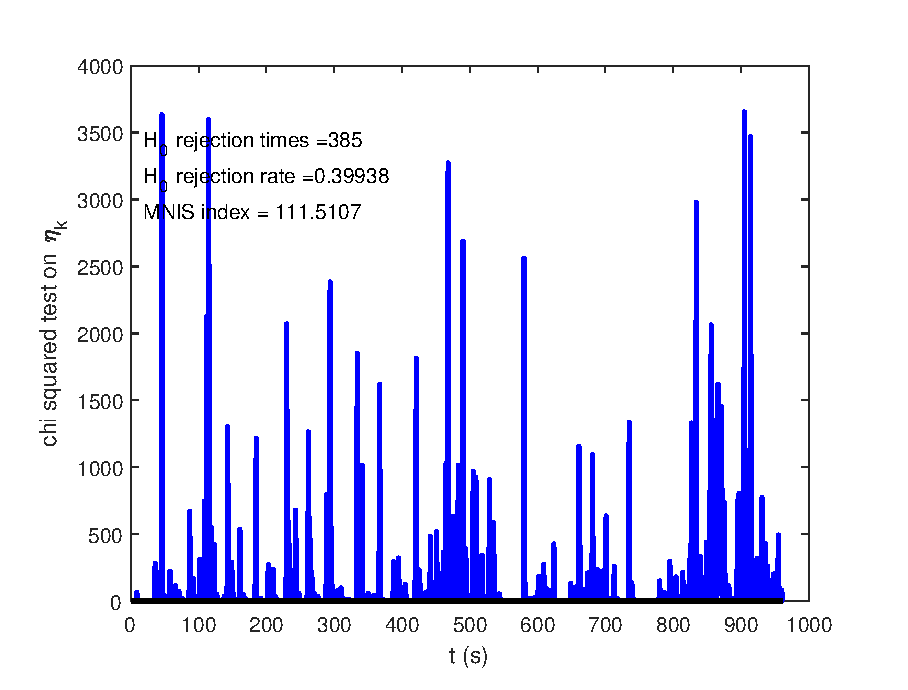
\includegraphics[width=.45\textwidth]{Imagens/chi_eta_without.eps}}
	\caption{First group of subfigures.}
	\label{fig:sub1}
\end{figure}






\subsection{Measurement Signal-to-Noise Ratio Variation}\label{sec:ruido-AC}

\subsubsection{Changing input and measurement noise jointly}

\begin{figure}[H]
	\centering
	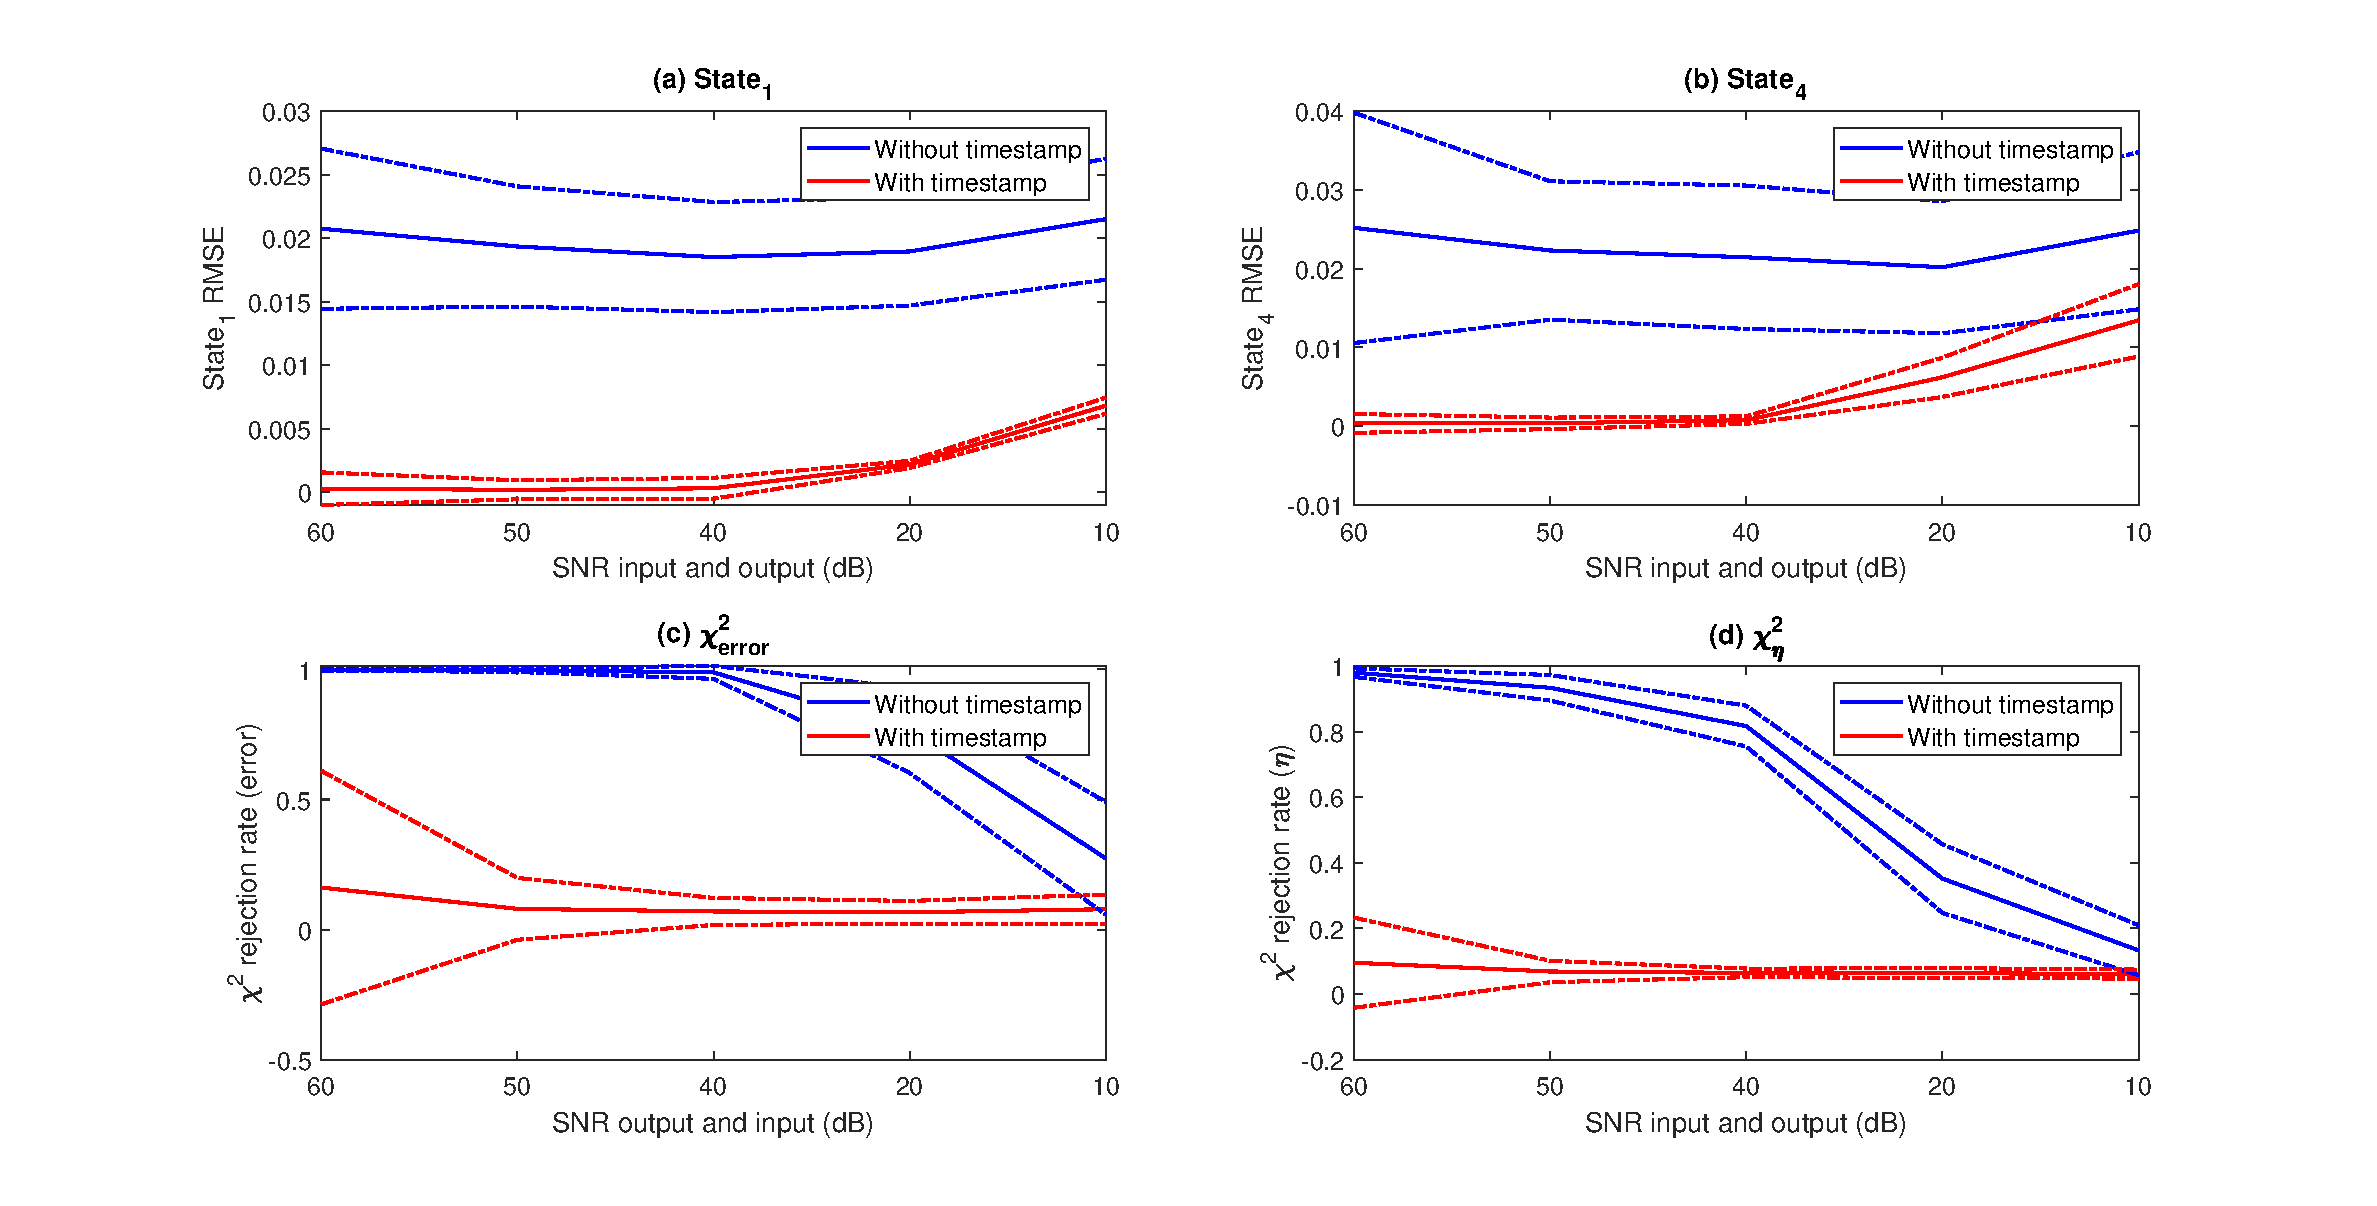
\includegraphics[width=1\textwidth]{Imagens/noise_results_all-uy.eps}
	\caption[entrada]{Performance, as a function of input and observation SNR}
	\label{fig:ulinearSamp}
\end{figure} 

\subsubsection{Changing only measurement noise}

\begin{figure}[H]
	\centering
	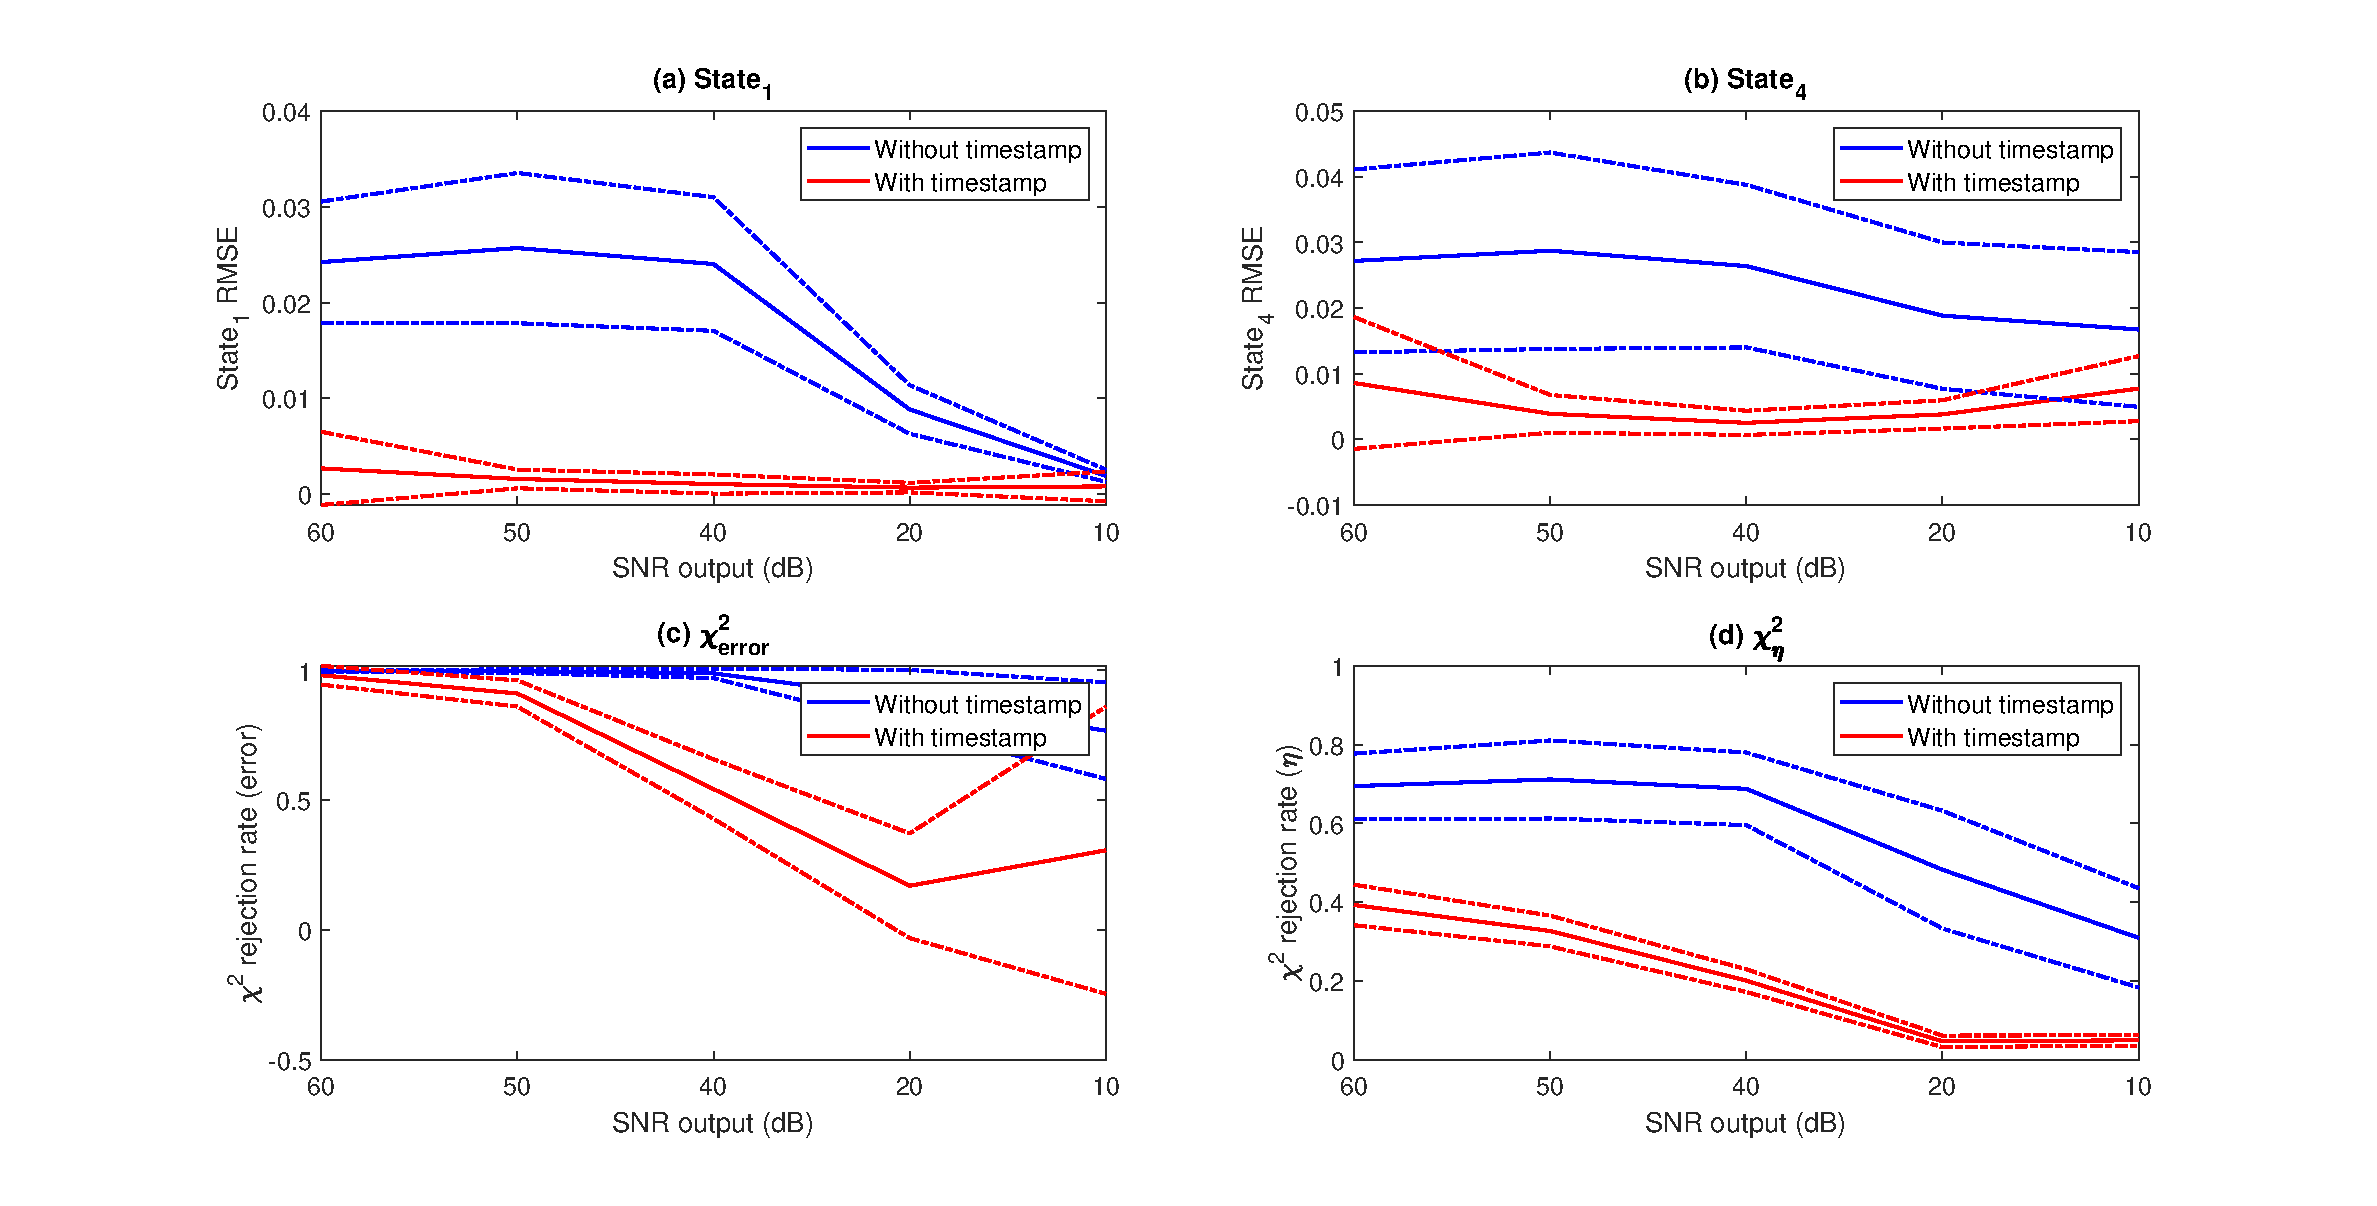
\includegraphics[width=1\textwidth]{Imagens/noise_results_all.eps}
	\caption[entrada]{Performance, as a function of observation SNR}
	\label{fig:ulinearSamp}
\end{figure} 



%	
%\begin{figure}[H]
%	\centering
%	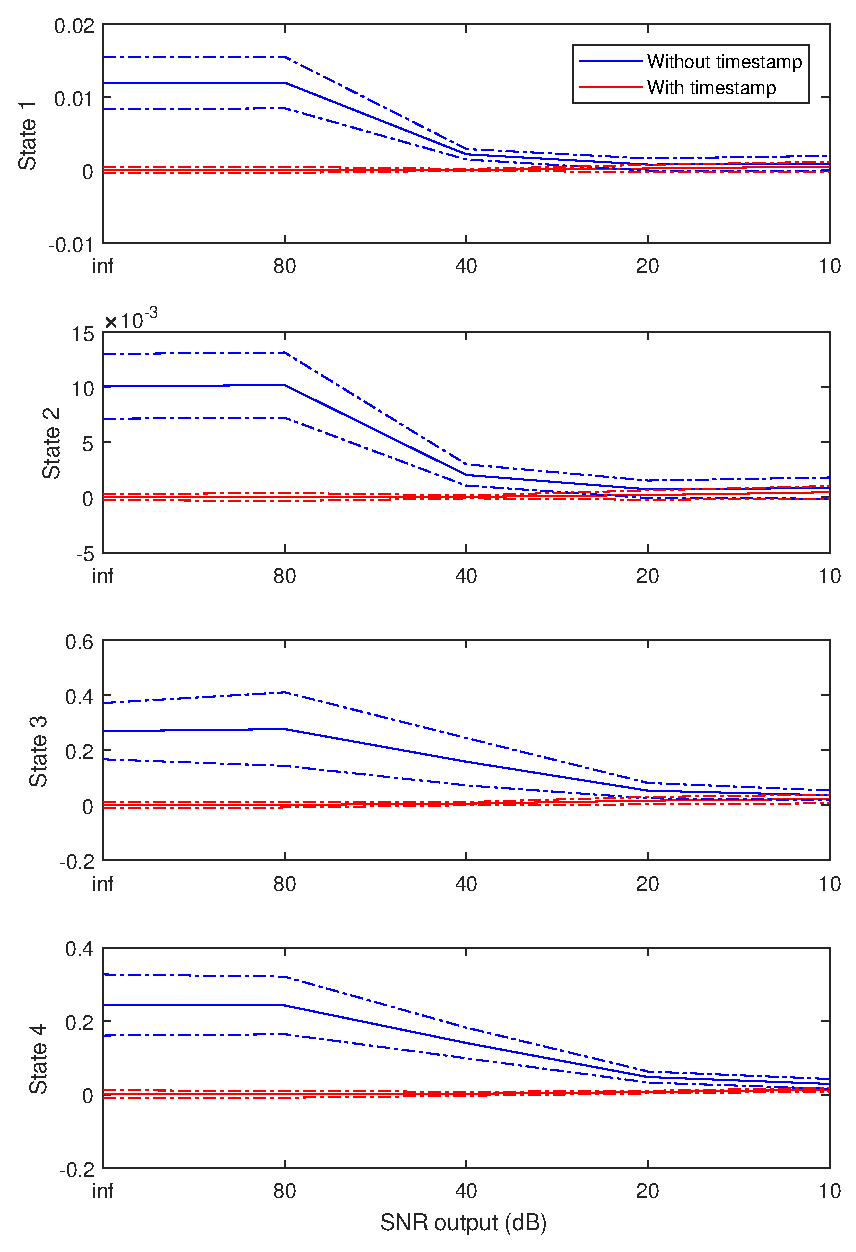
\includegraphics[width=0.8\textwidth]{Imagens/linearNoise.eps}
%	\caption[entrada]{Root mean square error variation, as a function of measurement noise for both KF algorithms, considering and not considering time-stamp}
%	\label{fig:linearNoise}
%\end{figure} 


\subsection{Average Sampling Rate Variation}\label{sec:lambda-AC}

\begin{figure}[H]
	\centering
	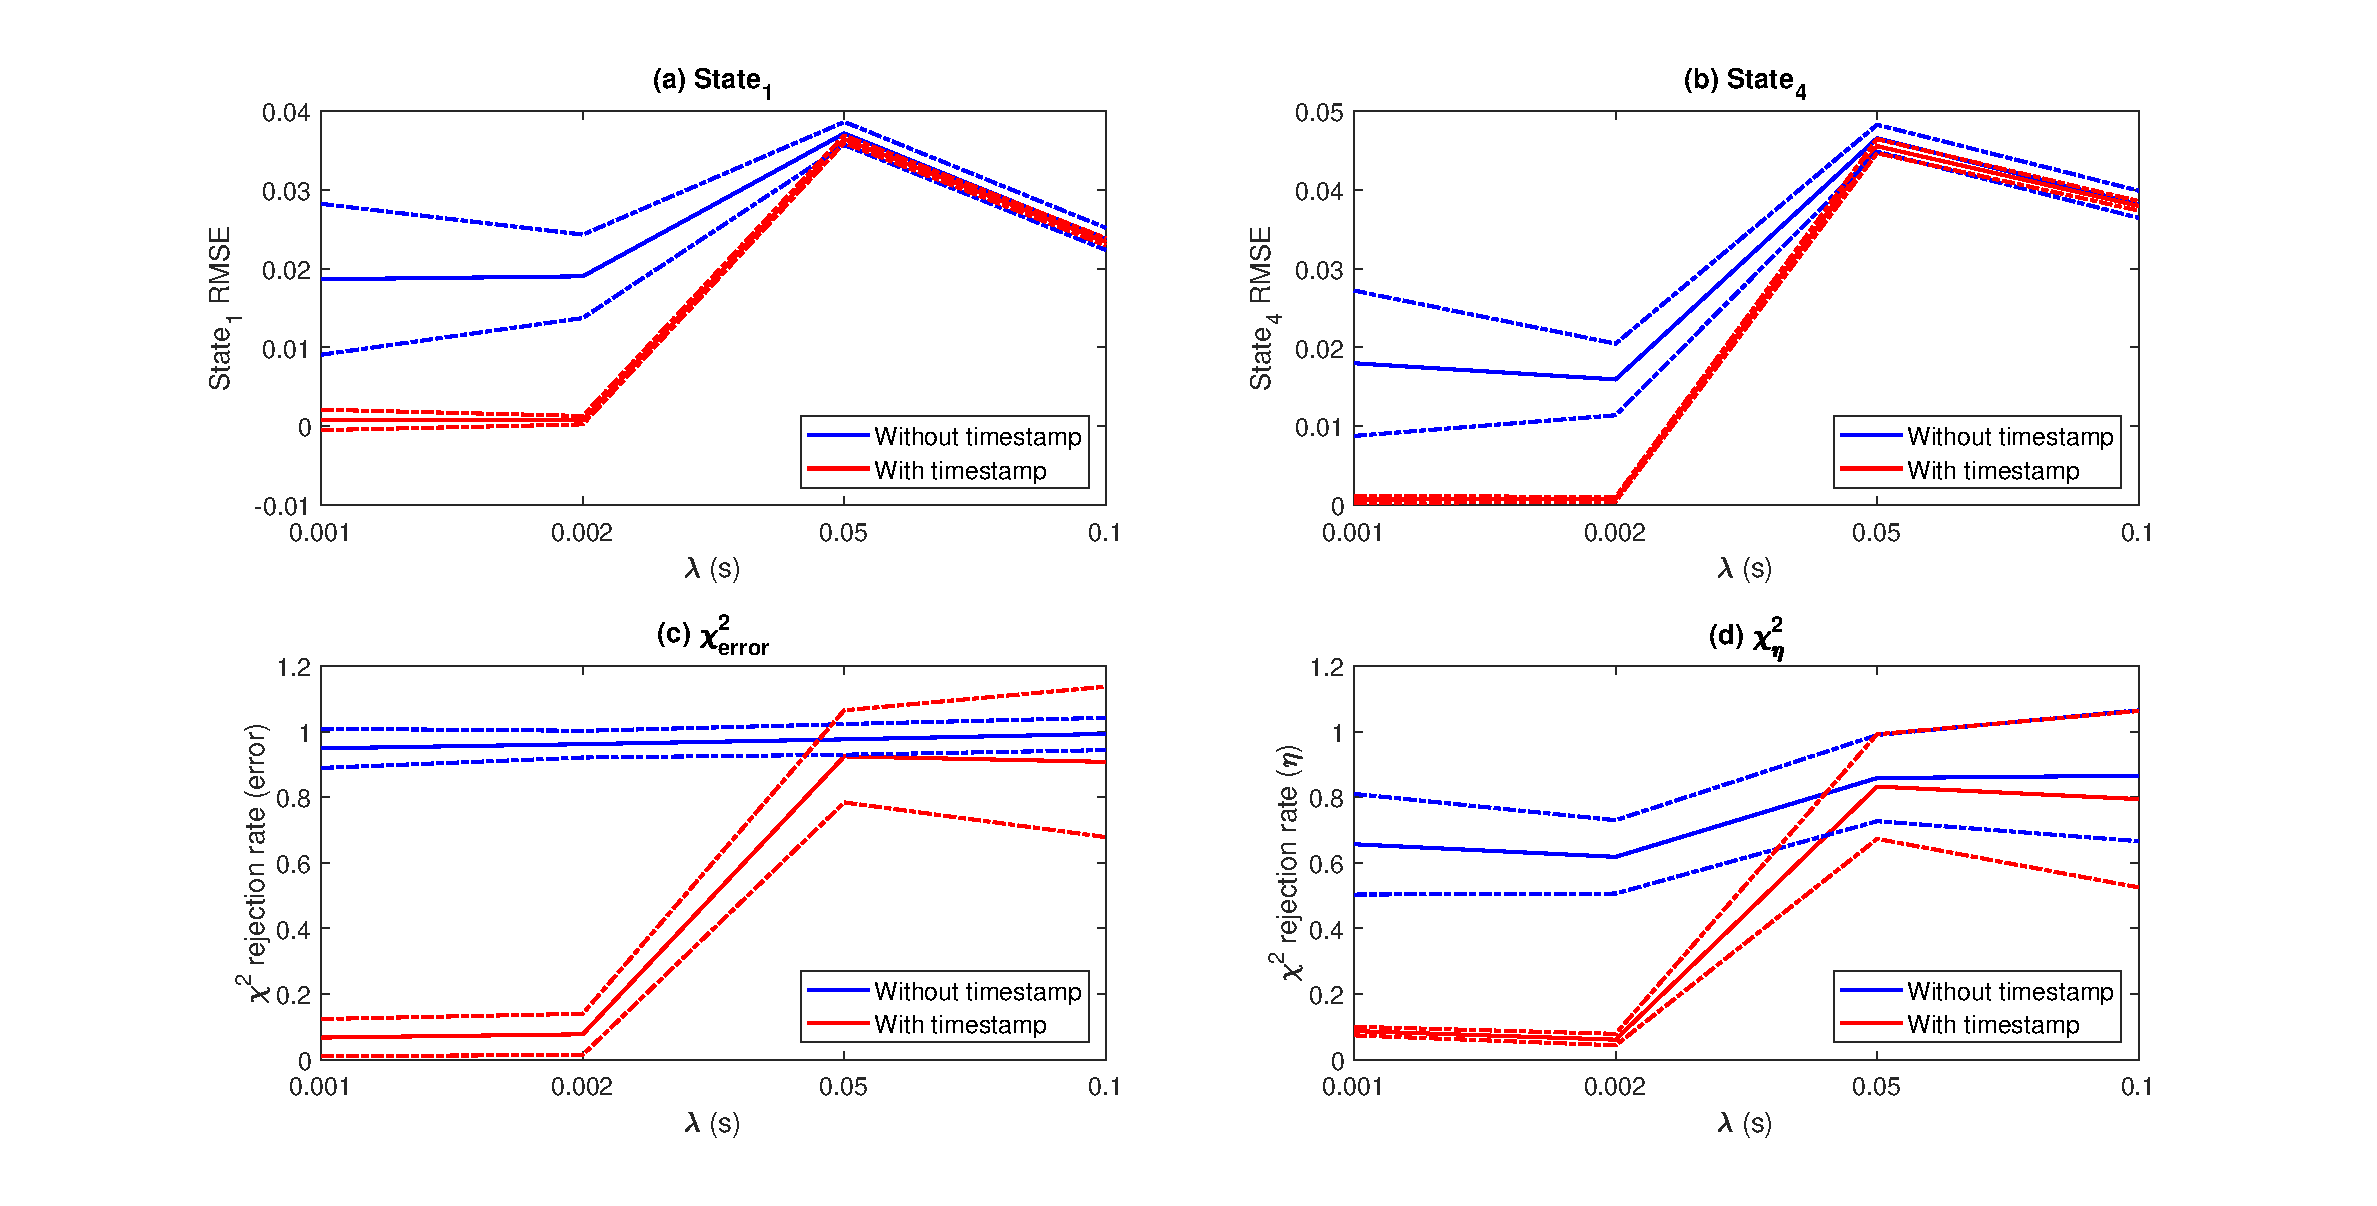
\includegraphics[width=1\textwidth]{Imagens/samp_results_all.eps}
	\caption[entrada]{Performance, as a function of $\lambda$}
	\label{fig:linearSamp}
\end{figure} 



\subsection{Regular and Average Irregular Time Interval Relation Variation}\label{sec:alpha-AC}

\begin{figure}[H]
	\centering
	\includegraphics[width=1\textwidth]{Imagens/usamp_results_all.eps}
	\caption[entrada]{Performance, as a function of $\alpha$}
	\label{fig:ulinearSamp}
\end{figure} 




\subsection{Average Time Delay}\label{sec:dt-AC}

\todo[inline,caption={Falta variar o atraso nas medi��es}]{Ainda ter� uma se��o com a varia��o do time-delay e seu impacto no desempenho}


\section{Unicycle Position Estimation}

\textit{Descrever as motiva��es por tr�s do estudo da amostragem irregular para problemas de rastreamento de rob�s. Exemplos: medi��es feitas por c�meras n�o sincronizadas e utilizando redes de internet (com time delay).}

\subsection{System Description}

Consider a nonholomonic moving robot, with the cinematic process model given by

\setlength{\abovedisplayskip}{0.5pt}

\begin{equation}\label{eq:sistema}
\begin{split}
\dot{p}_\textrm{x} & = v\cos (\theta),\\
\dot{p}_\textrm{y} & = v\sin (\theta),\\
\dot{\theta}  & = u_1(t),\\
\dot{v} & = u_2(t),
\end{split}
\end{equation}

\noindent
where $p_\textrm{x}$ and $p_\textrm{y}$ are the position coordinates, $\theta$ the angular orientation, $v$ the linear velocity and inputs $u_1$ and $u_2$ are the angular velocity $\omega$ and the linear acceleration $a$, respectively. Figure~\ref{fig:robot} shows a schematic of the robot and its states,

\begin{figure}[!htb]
	\centering
	\includegraphics[width=0.4\textwidth]{Imagens/Nonholomonic-robot.pdf}
	\caption[entrada]{Nonholomonic robot system representation. The system states $p_\textrm{x}$, $p_\textrm{y}$, $v$ and $\theta$ are highlighted.}
	\label{fig:robot}
\end{figure} 

The system described by~\ref{eq:sistema} is discretized by a 4$^{th}$ order Runge-Kutta method and the state vector $x_i$ is given by $x_i \overset{\Delta}{=} [p_{\textrm{x},i}\ p_{\textrm{y},i}\ \theta_i\ v_i]^T$.

The observation model $y(t_k) \in \mathbb{R}^2$

\begin{equation}
y(t_k) = 
\begin{bmatrix}
p_\textrm{x}(t_k) \\
p_\textrm{y}(t_k)
\end{bmatrix}+v(t_k), \\
\end{equation}

\noindent
is given by the position coordinates and $v(t_k) \sim \mathcal{N} (0,R_{t_k})$ is the observation noise, with zero mean and covariance $R_{t_k}$. When time-stamp is not available, the observation vector is approximated by $\tilde{y}_i \approx y(t_k)$, where $i$ is the index of the next time instant, multiple of $T$.

Input vector $u_i = [\omega_i\ a_i]^T$ is measured by a girometer and accelerometer, respectively. We assume that 

\begin{equation}\label{eq:entrada}
u_i = \tilde{u}_i - w_i,
\end{equation}

\noindent
where $\tilde{u}$ is the sensors measured valueand $w \sim \mathcal{N} (0, Q_i)$ represents the corresponded noise, of zero mean and covariance $Q_i$. 

We simulate 60 seconds of robot movement, considering a step size of $\delta t_{\textrm{sim}} = 10^{-4}$. Irregular sampling time intervals $h_k$ are simulated by the exponential probability distribution function from MatLab\texttrademark \ and approximated to the nearest discrete time instant, from the 600,000 available samples. Input signals were generated arbitrarily according to Figure~\ref{fig:entrada}. Figure~\ref{fig:exukf} shows robot trajectory on $xy$-plane for the given input signals, leaving from point $(0,0)$, as well as a realization of noisy and aperiodic measurements with signal-to-noise ratio of SNR\textsubscript{y} $= 30$ dB and $\lambda=0.3$ s as red dots and the hatched blue line represents UKF estimation, considering time-stamp, $\alpha=5$ and SNR\textsubscript{u} $= 10$ dB. 


\begin{figure}[!htb]
	\centering
	\begin{subfigure}
		\centering
		\includegraphics[width=\textwidth]{Imagens/entradas1.eps}	
		%		\caption{}
		\label{fig:sfig1}
	\end{subfigure}
	\begin{subfigure}
		\centering
		\includegraphics[width=\textwidth]{Imagens/entradas2.eps}
		%		\caption{}
		\label{fig:sfig2}
	\end{subfigure}
	\caption[Entradas]{Simulation input signals. (a) shows temporal sequence of angular velocity $\omega$ and (b) shows linear acceleration $a$.}
	\label{fig:entrada}
\end{figure}

\begin{figure}[!htb]
	\centering
	\includegraphics[width=0.8\textwidth]{Imagens/exemplo_03_30db_desloc.eps}
	\caption[entrada]{True position, noisy measurements and UKF estimates considering time-stamp, for a measurement noise of SNR\textsubscript{y} $= 30$ dB, $\lambda=0.3$ s and $\alpha=5$.}
	\label{fig:exukf}
\end{figure} 

To analyze the effect of considering time-stamp in the estimation algorithm, we use the performance index $J$

\begin{equation}\label{eq:inddesemp}
J = \frac{ \sum_{i=1}^N \sqrt{(\hat{p}_{\textrm{x},i}-p_{\textrm{x},i})^2+(\hat{p}_{\textrm{y},i}-p_{\textrm{y},i})^2}}{N}
\end{equation}

\noindent
where $\hat{p}_{\textrm{x},i}$ and $\hat{p}_{\textrm{y},i}$ are filter position estimates produced at a regular interval $T$, $\hat{p}_{\textrm{x},i}$ and $\hat{p}_{\textrm{y},i}$ the true coordinates of the robot at the same time instants and $N$ the total number of estimates. This index represents the average estimator position error in $xy$-plane.

Figure~\ref{fig:realizacaoJ} shows a timespan from 0 to 1.3 seconds of a $J$ realization, considering $\lambda=0.5$, $\alpha=5$, SNR\textsubscript{y} $=60dB$ dB and SNR\textsubscript{u} $=20$ dB, for the UKF considering and not considering time-stamp. Black dots represent the regular time instants $kT$ whereas the asterisks on x-axis match the exact measurement instants $t_k$. As expected, before the first data assimilation steps, both performances are identical. Since the first measurement $t_1$ was taken almost at the same time as regular estimation time instant $4T$, both estimation performances maintain close to each other. That is because the approximation error due to $\tilde{y}_i \approx y(t_k)$ is irrelevant. At $t_2$ we can observe significant deviation from index $J$ in benefit of the algorithm considering time-stamp, since it performs data assimilation at the exact time measurement was taken. The same effect can be noted at $t_4$, after 1 second of simulation, when there is a significant different between time the measurement was taken and the next regular estimation instant.


\begin{figure}[!htb]
	\centering
	\includegraphics[width=0.8\textwidth]{Imagens/J_umarealizacao.eps}
	\caption[entrada]{Temporal cut from 0 to 1.3 seconds, for a realization of $J$ of both estimators, with and without time-stamp. Asterisks on $x$ axis match the measurement sampling instants $t_k$. Black dots represent the regular estimation instants, same as input regular sampling instants.}
	\label{fig:realizacaoJ}
\end{figure} 

%\begin{figure}[!htb]
%	\centering
%	\includegraphics[width=0.8\textwidth]{Imagens/J_umarealizacao-timedelay.eps}
%%%	\caption[entrada]{Recorte temporal de 1 a 1.3 segundo, do �ndice J de uma realiza��o dos dois estimadores, com e sem carimbo de tempo. Os asteriscos no eixo $x$ representam os instantes de amostragem das observa��es $t_k$. Os pontos pretos apresentados nas linhas representam os instantes de tempo regulares de amostragem da entrada}
%	\label{fig:realizacaoJ2}
%\end{figure} 



%\setlength{\abovedisplayskip}{0.5pt}
%
%\begin{equation}\label{eq:sistema}
%\begin{split}
%\dot{\delta_e} & = -\tau^{-1},\\
%\dot{W} & = Z_{de}\delta_e + Z_wW + S_0q,\\
%\dot{q}  & = S_1 \delta_e + S_2 W + S_3q,\\
%\end{split}
%\end{equation}
%\noindent

\subsection{Measurement Signal-to-Noise Ratio Variation}\label{sec:ruido-robo}

In this subsection we compare the estimation performance impact of considering time-stamp in the algorithm, by varying the measurement noise level. The signal-to-noise ratio for the input sensors and the measurement average time interval are held constant, SNR\textsubscript{u} $= 20$ dB and $\lambda = 0.1$ s.

We considered an observation signal-to-noise variation of SNR\textsubscript{y} = $\infty$,  $80$, $60$, $40$, $20$, $10$ dB. That is, initially the system was simulated considering no measurement noise and then it was gradually increased. For each noise scenario, we ran 100 realizations of the random variables for each algorithm and Figure~\ref{fig:noise} shows the results. Solid lines represent the average values for $J$ and the dashed lines are the 95\% confidence interval.

\todo[inline]{Falta incluir resultados com time-delay}


\begin{figure}[!htb]
	\centering
	\includegraphics[width=0.8\textwidth]{Imagens/noise.eps}
	\caption[entrada]{Performance index $J$ variation, as a function of measurement noise for both UKF algorithms considering and not considering time-stamp}
	\label{fig:noise}
\end{figure} 


\textit{� poss�vel observar que o estimador que considera o carimbo de tempo possui desempenho estatisticamente superior apenas para baixos n�veis de ru�do da observa��o. Quando SNR\textsubscript{y} � igual a $\infty$ e $80$ dB, o �ndice de desempenho $J$ do filtro com carimbo de tempo � aproximadamente $1.25$ e $1.26$ cm, respectivamente, mais preciso do que sem carimbo de tempo e com vari�ncia pequena. Quando a rela��o sinal ru�do se aproxima de $40$ dB, no entanto, n�o � poss�vel distinguir estatisticamente o efeito de se considerar ou n�o carimbo de tempo.
}


\subsection{Average Sampling Rate Variation}\label{sec:lambda-robot}

We now consider the variation of the average time interval that observations are taken, according to $\lambda =$ $0.1$, $0.2$, $0.3$, $0.4$, $0.5$, $0.6$ s, maintaining the other parameters constant, namely the noise level of inputs and observations, SNR\textsubscript{u} $= 20$ dB and SNR\textsubscript{y} $= 40$ dB, respectively. We carried out 100 realizations for each $\lambda$ and for each algorithm and Figure~\ref{fig:samp} presents the results. Again, the solid lines are the average values of $J$ and the 95\% confidence interval is between the dashed lines.

\begin{figure}[!htb]
	\centering
	\includegraphics[width=0.8\textwidth]{Imagens/samp.eps}
	\caption[entrada]{Performance index $J$ variation, as a function of measurement noise both UKF algorithms considering and not considering time-stamp}
	\label{fig:samp}
\end{figure}


\textit{Os resultados obtidos demonstram que a diferen�a no desempenho dos filtros � mais significativa para intervalos de tempo mais espa�ados, mantendo-se a din�mica do sistema e os outros par�metros fixos. Inicialmente, para valores pequenos de $\lambda$	, n�o h� diferen�a estat�stica entre o desempenho dos estimadores, mas a medida que o intervalo cresce, ela aparece, chegando a aproximadamente $3.1$ cm para um $\lambda = 0.6$ s. Uma interpreta��o poss�vel � que, se o intervalo de tempo m�dio das observa��es for muito pequeno em compara��o com a velocidade em que a din�mica do sistema varia, o erro de aproxima��o do instante de amostragem das observa��es $t_k$ � reduzido. O ru�do do sensor pode acabar sendo mais relevante do que o erro devido ao tempo incorreto de assimila��o.}


\subsection{Regular and Average Irregular Time Interval Relation Variation}\label{sec:alpha-robot}

We also analyze the performance impact of varying the parameter $\alpha$, which is the relation between regular input time interval $T$ and average measurements time interval $\lambda$. The simulated values were $\alpha = 10$, $5$, $2$, $1$. That means we start with higher frequency values for input sampling in comparison to measurement sampling and this values is gradually decreased. Other parameters were maintained constant SNR\textsubscript{u} $= 20$ dB and SNR\textsubscript{y} $= 40$ dB.

The same way we did for the other scenarios, 100 realizations were simulated and Figure~\ref{fig:dtudty} presents the results. Solid lines are the average values for $J$ and dashed lines represent the 95\% confidence interval.

\begin{figure}[!htb]
	\centering
	\includegraphics[width=0.8\textwidth]{Imagens/dtudty.eps}
	\caption[entrada]{Performance index $J$ variation, as a function of measurement noise both UKF algorithms considering and not considering time-stamp}
	\label{fig:dtudty}
\end{figure}


\textit{
	Nota-se que, quando o carimbo de tempo � considerado, n�o h� diferen�a significativa em se variar o $\alpha$ no desempenho do filtro, com o �ndice de desempenho $J$ se mantendo pouco abaixo dos $3$ cm. Ou seja, n�o importa a rela��o entre as frequ�ncias de amostragem da observa��o e das entradas. Por outro lado, quando n�o se considera o carimbo de tempo, essa rela��o se torna relevante para o �ndice de desempenho do estimador. Quanto mais lento a frequ�ncia da entrada em compara��o com a frequ�ncia da sa�da, maior o erro obtido. Para o caso mais extremo utilizado, $\alpha=1$, a diferen�a no �ndice $J$ foi mais do que o dobro. Esse resultado era esperado, uma vez que quanto maior o valor de $\alpha$, mais r�pida � a taxa de discretiza��o do modelo de processo em rela��o � frequ�ncia dos sensores de observa��o. Consequentemente, o erro obtido na aproxima��o $\tilde{y}(i) \approx y(t_k)$ diminui.
}

\subsection{Average Time Delay}\label{sec:dt-robot}

\todo[inline,caption={Falta variar o atraso nas medi��es}]{Ainda ter� uma se��o com a varia��o do time-delay e seu impacto no desempenho}


\clearpage

\clearpage
\thispagestyle{empty}
\cleardoublepage

%Cap�tulo 5 - Conclusions
%-------------------------------------------------------------------------------
\chapter{Conclusions}
\label{cap6} \vspace{-1cm} \vspace{1cm}

%\begin{flushright}
%\begin{minipage}{0.7\linewidth}
%\emph{``Enquanto existir vontade de lutar, existem esperan�as de
%vencer.''}
%\end{minipage}
%\end{flushright}
%
%\begin{flushright}
%{A. Agostinho}
%\end{flushright}


\section{Project Overview}

Investigou-se isso e aquilo... (caso algum leitor pule direto para a conclus�o)

\section{Main Results}

Como os resultados corroboram os objetivos perseguidos. O que � relevante dizer sobre cada objetivo descrito no cap�tulo 1, com o que foi feito no trabalho.

Autocr�tica sobre o trabalho: alguma hip�tese foi pouco realista? o que n�o foi feito t�o bem? o que foi feito bem?

\section{Future Work}
Talvez uma lista itemizada
Trabalhos futuros podem vir diretamente da autocr�tica.


\clearpage

\clearpage
\thispagestyle{empty}
\cleardoublepage
%
%--------------------------------------------------------------------
%--------------------------------------------------------------------
%Bibliografia
%--------------------------------------------------------------------
%Defini��o de cabe�alhos
\bibliographystyle{apalike} %plainnat_mod
\bibliography{library}
\addcontentsline{toc}{chapter}{References}
 \clearpage
\thispagestyle{empty}
%\cleardoublepage

%Ap�ndices
%\appendix
%\begin{center}
\appendix{-- \ \ Arquivos do analisador simbólico-numérico}\label{ApendiceA}
\end{center}



\section{Arquivo do analisador léxico}\label{ApendiceA:Lex}

\lstinputlisting[language=Perl, label=sources:AnalisadorLexico, caption={Arquivo para geração de
um analisador léxico}]{./apendices/sources/calculator.l}


\section{Arquivo do analisador sintático}\label{ApendiceA:Sintatico}

\lstinputlisting[language=Perl, label=sources:AnalisadorSintatico, caption={Arquivo para geração de
um analisador sintático}]{./apendices/sources/calculator.y}


\section{Arquivo de interface entre o $hp^2$FEM e o analisador
simbólico-numérico}\label{ApendiceA:Analisador}

\lstinputlisting[language=Perl, label=sources:AnalisadorSintatico, caption={Arquivo de interface
entre o \textit{software} $hp^2$FEM e o analisador
simbólico-numérico}]{./apendices/sources/calculator.y}



% Apêndices\index{apêndices} complementam o texto principal da tese com informações para leitores com
% especial interesse no tema, devendo ser considerados leitura opcional, ou seja, o entendimento do
% texto principal da tese não deve exigir a leitura atenta dos apêndices.
% 
% Apêndices usualmente contemplam provas de teoremas, deduções de fórmulas\index{fórmulas}
% matemáticas\index{fórmulas!matemáticas}, diagramas esquemáticos, gráficos e trechos de código.
% Quanto a este último, código extenso não deve fazer parte da tese, mesmo como apêndice. O ideal é
% disponibilizar o código na Internet para os interessados em examiná-lo ou utilizá-lo.
% 
% \section{Seção do apêndice}
% Equação:
% \begin{equation}\label{eq:WTS}
% w_i=X_{1}^i(x_1)t \ldots tX_{n}^i(x_n)
% \end{equation}

%\clearpage
%\thispagestyle{empty}
%\cleardoublepage

%
% \chapter{Demonstra��es}
 %\appendix
%\chapter{Demonstra��es}
\label{B}
\section{Demonstra��o - Equa��es Matriciais Entrada-Sa�da}\label{eqmat_in_out}
Num primeiro momento ser� provada a equa��o (\ref{y_past_det}).
Portanto, considere o vetor de sa�das que varia de $k$ at� $k+i-1$:

\begin{equation}
\textbf{y}_k=\left[y_k~y_{k+1}~\cdots~y_{k+i-1}\right]^{T},
\end{equation}
em que $i>n$. Assim, de (\ref{mat_y}), tem-se que:
\begin{eqnarray}
y_{k+1}&=Cx_{k+1} + Du_{k+1}=C(Ax_{k} + Bu_{k}) +
Du_{k+1}\nonumber\\
&= CAx_{k} + \left[\begin{array}{cc}
                       CB & D
                     \end{array}
\right] \left[\begin{array}{c}
                u_{k} \\
                u_{k+1}
              \end{array}\right],~~~~~~~~~~~~~~~~\label{y_k_1_teo1}
\end{eqnarray}
e,
\begin{eqnarray}
x_{k+2}&=Ax_{k+1} + Bu_{k+1} = A(Ax_{k} + Bu_{k}) +
Bu_{k+1}= A^{2}x_{k}+ ABu_{k}+ Bu_{k+1},\\
y_{k+2}&=Cx_{k+2} + Du_{k+2}=C(A^{2}x_{k}+ ABu_{k}+
Bu_{k+1})+ Du_{k+2}\nonumber~~~~~~~~~~~~~~~~~~~~~~\\
&= CA^{2}x_{k} + \left[\begin{array}{ccc}
                                             CAB & CB & D
                                           \end{array}\right]\left[ \begin{array}{c}
                        u_{k} \\
                        u_{k+1} \\
                        u_{k+2}
                      \end{array}
 \right].~~~~~~~~~~~~~~~~~~~~~~~~~~~~~~~~~~~~~~~~~~~~~~\label{y_k_2_teo1}
\end{eqnarray}

Seguindo o mesmo procedimento at� $k+i-1$, obt�m-se:

\begin{equation}\label{y_k_i_1_teo1}
y_{k+i-1}=CA^{i-1}x_{k}+ \left[\begin{array}{cccccc}
                                       CA^{i-2}B & CA^{i-3}B & CA^{i-4}B& \cdots & CB &
                                       D
                                     \end{array}
\right]\left[\begin{array}{c}
                u_{k} \\
                u_{k+1} \\
                u_{k+2} \\
               \vdots \\
                u_{k+i-2} \\
                u_{k+i-1}
             \end{array}
 \right].
\end{equation}

Colocando as equa��es (\ref{mat_y}), (\ref{y_k_1_teo1}),
(\ref{y_k_2_teo1}) e (\ref{y_k_i_1_teo1}) na forma matricial,
tem-se:
\begin{eqnarray}
\left[\begin{array}{c}
        y_{k} \\
        y_{k+1} \\
        y_{k+2} \\
        \vdots \\
        y_{k+i-1}
      \end{array}
\right]_{li \times 1}&=&\left[\begin{array}{c}
        C \\
        CA \\
       CA^{2} \\
       \vdots\\
       CA^{i-1}
      \end{array}
\right]_{li \times n}\left[x_{k}\right]_{n \times 1}+\nonumber\\
&+&\left[\begin{array}{ccccc}
           D & 0 & 0 & 0 \cdots & 0 \\
           CB & D & 0 & \cdots & 0 \\
           CAB & CB & D & \ddots & 0 \\
           \vdots & \vdots & \vdots & \ddots & \vdots \\
           CA^{i-2}B & CA^{i-3}B & CA^{i-4}B  & \cdots & D
         \end{array}
\right]_{li \times mi}\left[\begin{array}{c}
                              u_{k} \\
                              u_{k+1} \\
                              u_{k+2} \\
                              \vdots \\
                              u_{k+i-1}
                            \end{array}
\right]_{mi \times 1}.
\end{eqnarray}

Empregando-se nota��o de matriz de observabilidade estendida
(\ref{observabilidade_estendida_1}) e de matriz em blocos triangular
inferior de Toeplitz (\ref{toeplitz_det}), obt�m-se:

\begin{equation}
\left[\begin{array}{c}
        y_{k} \\
        y_{k+1} \\
        y_{k+2} \\
        \vdots \\
        y_{k+i-1}
      \end{array}
\right]=\Gamma_{i}x_{k}+H^{d}_{i}\left[\begin{array}{c}
                              u_{k} \\
                              u_{k+1} \\
                              u_{k+2} \\
                              \vdots \\
                              u_{k+i-1}
                            \end{array}
\right].
\end{equation}

Em seguida, varia-se $k$ de $0$ a $j-1$, como a seguir:
\begin{flushleft}
\begin{minipage}{10.75cm}
\begin{eqnarray}
&\text{\normalsize{Para $k=0$,~ent�o}}&\left[\begin{array}{c}
        y_{0} \\
        y_{1} \\
        y_{2} \\
        \vdots \\
        y_{i-1}
      \end{array}
\right]=\Gamma_{i}x_{0}+H^{d}_{i}\left[\begin{array}{c}
                              u_{0} \\
                              u_{1} \\
                              u_{2} \\
                              \vdots \\
                              u_{i-1}
                            \end{array}
\right],\nonumber\\
&\text{\normalsize{Para $k=1$,~ent�o}}&\left[\begin{array}{c}
        y_{1} \\
        y_{2} \\
        y_{3} \\
        \vdots \\
        y_{i}
      \end{array}
\right]=\Gamma_{i}x_{1}+H^{d}_{i}\left[\begin{array}{c}
                              u_{1} \\
                              u_{2} \\
                              u_{3} \\
                              \vdots \\
                              u_{i}
                            \end{array}
\right],\nonumber\\
&\text{\normalsize{Para $k=j-1$,~ent�o}}&\left[\begin{array}{c}
        y_{j-1} \\
        y_{j} \\
        y_{j+1} \\
        \vdots \\
        y_{i+j-2}
      \end{array}
\right]=\Gamma_{i}x_{j-1}+H^{d}_{i}\left[\begin{array}{c}
                              u_{j-1} \\
                              u_{j} \\
                              u_{j+1} \\
                              \vdots \\
                              u_{i+j-2}
                            \end{array}
\right].\nonumber
\end{eqnarray}
\end{minipage}
\end{flushleft}

Expressando essas equa��es em matrizes de blocos, obt�m-se:

\begin{eqnarray}
\left[\begin{array}{cccc}
        y_{0} & y_{1} & \cdots & y_{j-1} \\
        y_{1} & y_{2} & \cdots & y_{j} \\
        y_{2} & y_{3} & \cdots & y_{j+1} \\
        \vdots & \vdots & \cdots & \vdots \\
        y_{i-1} & y_{i} & \cdots & y_{i+j-2}
      \end{array}
\right]&=&\Gamma_{i}\left[\begin{array}{ccccc}
                            x_{0} & x_{1} & \cdots & x_{j-2} & x_{j-1}
                          \end{array}
\right]+\nonumber\\
&+&H^{d}_{i}\left[\begin{array}{cccc}
        u_{0} & u_{1} & \cdots & u_{j-1} \\
        u_{1} & u_{2} & \cdots & u_{j} \\
        u_{2} & u_{3} & \cdots & u_{j+1} \\
        \vdots & \vdots & \cdots & \vdots \\
        u_{i-1} & u_{i} & \cdots & u_{i+j-2}
      \end{array}\right].
\end{eqnarray}

Portanto, pode-se concluir que:
\begin{equation}
   Y_{p}=\Gamma_{i}X_{p} + H^{d}_{i}U_{p}.\nonumber
\end{equation}

Agora ser� provada a equa��o (\ref{y_future_det}). Considere o
seguinte vetor de sa�das que varia de $k+i$ at� $k+2i-1$:

\begin{equation}
\textbf{y}_{k+i}=\left[y_{k+i}~y_{k+i+1}~\cdots~y_{k+2i-1}\right]^{T},
\end{equation}
em que $i>n$. Seguindo o mesmo racioc�nio utilizado para provar
(\ref{y_past_det}), fazendo-se substitui��es sucessivas para cada
medida do vetor $\textbf{y}_{k+i}$, obt�m-se:

\begin{eqnarray}
\left[\begin{array}{c}
        y_{k+i} \\
        y_{k+i+1} \\
        y_{k+i+2} \\
        \vdots \\
        y_{k+2i-1}
      \end{array}
\right]_{li \times 1}&=&\left[\begin{array}{c}
        C \\
        CA \\
       CA^{2} \\
       \vdots\\
       CA^{i-1}
      \end{array}
\right]_{li \times n}\left[x_{k+i}\right]_{n \times 1}+\nonumber\\
&+&\left[\begin{array}{ccccc}
           D & 0 & 0 & 0 \cdots & 0 \\
           CB & D & 0 & \cdots & 0 \\
           CAB & CB & D & \ddots & 0 \\
           \vdots & \vdots & \vdots & \ddots & \vdots \\
           CA^{i-2}B & CA^{i-3}B & CA^{i-4}B  & \cdots & D
         \end{array}
\right]_{li \times mi}\left[\begin{array}{c}
                              u_{k+i} \\
                              u_{k+i+1} \\
                              u_{k+i+2} \\
                              \vdots \\
                              u_{k+2i-1}
                            \end{array}
\right]_{mi \times 1}.
\end{eqnarray}

Variando-se $k$ de $0$ a $j-1$ e expressando as equa��es resultantes
na forma de matrizes de blocos, resulta em:

\begin{eqnarray}
\left[\begin{array}{cccc}
        y_{i} & y_{i+1} & \cdots & y_{i+j-1} \\
        y_{i+1} & y_{i+2} & \cdots & y_{i+j} \\
        y_{i+2} & y_{i+3} & \cdots & y_{i+j+1} \\
        \vdots & \vdots & \cdots & \vdots \\
        y_{2i-1} & y_{2i} & \cdots & y_{2i+j-2}
      \end{array}
\right]&=&\Gamma_{i}\left[\begin{array}{ccccc}
                            x_{i} & x_{i+1} & \cdots & x_{i+j-2} & x_{i+j-1}
                          \end{array}
\right]+\nonumber\\
&+&H^{d}_{i}\left[\begin{array}{cccc}
        u_{i} & u_{i+1} & \cdots & u_{i+j-1} \\
        u_{i+1} & u_{i+2} & \cdots & u_{i+j} \\
        u_{i+2} & u_{i+3} & \cdots & u_{i+j+1} \\
        \vdots & \vdots & \cdots & \vdots \\
        u_{2i-1} & u_{2i} & \cdots & u_{2i+j-2}
      \end{array}\right].
\end{eqnarray}

Dessa forma, conclui-se que:

\begin{equation}
   Y_{f}=\Gamma_{i}X_{f} + H^{d}_{i}U_{f}. \nonumber
\end{equation}

Por fim, ser� provada a equa��o (\ref{x_future_det}). Expandindo-se
a equa��o (\ref{mat_x}), obt�m-se:

\begin{eqnarray}
x_{k+1}&=&Ax_{k} + Bu_{k},\\
x_{k+2}&=& A^{2}x_{k}+ ABu_{k}+ Bu_{k+1},\\
x_{k+3}&=& A^{3}x_{k}+A^{2}Bu_{k}+  ABu_{k+1}+ Bu_{k+2},\\
\cdots&~~~~~~~~~~&\cdots~~~~~~~~~~\cdots~~~~~~~~~~\cdots~~~~~~~~~~\cdots\nonumber\\
x_{k+i-1}&=& A^{i-1}x_{k}+A^{i-2}Bu_{k}+
A^{i-3}Bu_{k+1}+\ldots ABu_{k+i-3}+Bu_{k+i-2},\\
x_{k+i}&=& A^{i}x_{k}+A^{i-1}Bu_{k}+ A^{i-2}Bu_{k+1}+\ldots
ABu_{k+i-2}+Bu_{k+i-1}.\label{ext_dedu}
\end{eqnarray}

A equa��o (\ref{ext_dedu}) pode ser expressa como a seguir:
\begin{equation}
x_{k+i}=\left[\begin{array}{c}
                    A^{i}
                  \end{array}
\right]_{n\times n}\left[\begin{array}{c}
                    x_{k}
                  \end{array}\right]_{n\times 1} +
\left[\begin{array}{c|c|c|c|c}
             A^{i-1}B & A^{i-2}B & \cdots & AB & B
           \end{array}
\right]_{n \times mi}\left[\begin{array}{c}
                             u_{k} \\
                             u_{k+1} \\
                             \vdots  \\
                              u_{k+i-2}\\
                              u_{k+i-1}
                           \end{array}
\right]_{mi \times 1}.
\end{equation}

Empregando-se nota��o de matriz de controlabilidade estendida
(\ref{controlabilidade_estendida_det}), obt�m-se:
\begin{equation}
x_{k+i}=A^{i}x_{k}+\Delta^{d}_{i}\left[\begin{array}{c}
                             u_{k} \\
                             u_{k+1} \\
                             \vdots  \\
                              u_{k+i-2}\\
                              u_{k+i-1}
                           \end{array}
\right].
\end{equation}

Variando-se $k$ de $0$ a $j-1$, obt�m-se a seguinte equa��o na forma
de matrizes de blocos:

\begin{eqnarray}
\left[\begin{array}{ccccc}\label{x_future_det_demo}
                            x_{i} & x_{i+1} & \cdots & x_{i+j-2} & x_{i+j-1}
                          \end{array}
\right]&=&A^{i}\left[\begin{array}{ccccc}
                            x_{0} & x_{1} & \cdots & x_{j-2} & x_{j-1}
                          \end{array}
\right]+\nonumber\\
&+&\Delta^{d}_{i}\left[\begin{array}{cccc}
        u_{0} & u_{1} & \cdots & u_{j-1} \\
        u_{1} & u_{2} & \cdots & u_{j} \\
        u_{2} & u_{3} & \cdots & u_{j+1} \\
        \vdots & \vdots & \cdots & \vdots \\
        u_{i-1} & u_{i} & \cdots & u_{i+j-2}
      \end{array}\right].
\end{eqnarray}

Portanto a equa��o (\ref{x_future_det_demo}), pode ser expressa como
(\ref{x_future_det}):
\begin{equation}
   X_{f}=A^{i}X_{p} + \Delta^{d}_{i}U_{p}.\nonumber
\end{equation}
\begin{flushright}
$\Box$
\end{flushright}
\section{Demonstra��o - Teorema \ref{teo_2}}\label{demons_teo_2}

Deseja-se escrever os estados futuros $X_{f}$ como uma combina��o
linear dos dados de entradas passadas e futuras. Isto pode ser
obtido relacionando as equa��es (\ref{y_past_det}) e
(\ref{x_future_det}). Para este desenvolvimento � necess�rio
explicitar os $X_{p}$ na equa��o (\ref{x_future_det}) para, ent�o,
substitu�-los na equa��o (\ref{y_past_det}). Contudo, a matriz
$\Gamma_{i} \in \mathbb{R}^{li \times n}$ n�o � quadrada,
portanto n�o pode ser invertida. Sendo assim, %ser� utilizado um
%artif�cio amplamente conhecido em identifica��o de sistemas
%(\cite{Aguir2007}). Em um primeiro momento,
pr�-multiplicando a equa��o (\ref{y_past_det}) por $\Gamma^{T}_{i}$
de ambos os lados, resulta em

\begin{equation}\label{y_p_multi_gamma_t}
\Gamma^{T}_{i}Y_{p} =
\Gamma^{T}_{i}\Gamma_{i}X_{p}+\Gamma^{T}_{i}H^{d}_{i}U_{p}.
\end{equation}

Reorganizando (\ref{y_p_multi_gamma_t}), obt�m-se
\begin{equation}
\Gamma^{T}_{i}\Gamma_{i}X_{p}=\Gamma^{T}_{i}Y_{p}
-\Gamma^{T}_{i}H^{d}_{i}U_{p}.
\end{equation}

Tem-se que o produto de uma matriz pela sua transposta � uma matriz
quadrada, supondo-se que $\left[\Gamma^{T}_{i}\Gamma_{i}\right]$
seja n�o singular, obt�m-se a seguinte express�o

\begin{equation}\label{x_p_proof_det}
X_{p}=\left[\Gamma^{T}_{i}\Gamma_{i}\right]^{-1}\Gamma^{T}_{i}Y_{p}
-\left[\Gamma^{T}_{i}\Gamma_{i}\right]^{-1}\Gamma^{T}_{i}H^{d}_{i}U_{p}.
\end{equation}

A matriz $\left[\Gamma^{T}_{i}\Gamma_{i}\right]^{-1}\Gamma^{T}_{i}$
� conhecida como matriz pseudo-inversa de Moore-Penrose de
$\Gamma_{i}$ e � denotada por
$\Gamma^{\dag}_{i}\triangleq\left[\Gamma^{T}_{i}\Gamma_{i}\right]^{-1}\Gamma^{T}_{i}$.
Ent�o a equa��o (\ref{x_p_proof_det}) pode ser reescrita como
\begin{equation}\label{x_d_p_mod}
X_{p}=\Gamma^{\dag}_{i}Y_{p} -\Gamma^{\dag}_{i}H^{d}_{i}U_{p}.
\end{equation}

Logo, substituindo-se (\ref{x_d_p_mod}) em (\ref{x_future_det}),
obt�m-se:
\begin{eqnarray}
X_{f}&=&A^{i}(\Gamma^{\dag}_{i}Y_{p}
-\Gamma^{\dag}_{i}H^{d}_{i}U_{p})
+ \Delta^{d}_{i}U_{p}, \nonumber\\
&=&(\Delta^{d}_{i}-A^{i}\Gamma^{\dag}_{i}H^{d}_{i})U_{p}+(A^{i}\Gamma^{\dag}_{i})Y_{p}.\label{x_f_d_mod}
\end{eqnarray}

Por fim, colocando (\ref{x_f_d_mod}) na forma de matriz, tem-se que:

\begin{equation}\label{xdf_analog}
X_{f}=\left[\begin{array}{cc}
                  \Delta^{d}_{i}-A^{i}\Gamma^{\dag}_{i}H^{d}_{i} & A^{i}\Gamma^{\dag}_{i}
                \end{array}
\right]\left[\begin{array}{c}
                U_{p} \\
                Y_{p}
              \end{array}
\right].
\end{equation}

Como mostrado na equa��o (\ref{xdf_analog}) os estados futuros est�o
contidos nos dados de entradas e sa�das passados. Agora, ser�
mostrado que estes estados n�o est�o somente contidos nos dados de
entradas e sa�das passadas, mas tamb�m nos dados de entradas e
sa�das futuras. Essa demonstra��o, naturalmente, mostra como os
estados s�o obtidos por meio dos dados medidos. De
(\ref{xdf_analog}), pode-se fazer a seguinte analogia

\begin{equation}\label{x_f_d_comb}
X_{f}=L_{p}W_{p},
\end{equation}
com
\begin{equation}
L_{p}=\left[\begin{array}{cc}
                  \Delta^{d}_{i}-A^{i}\Gamma^{\dag}_{i}H^{d}_{i} & A^{i}\Gamma^{\dag}_{i}
                \end{array}
\right].
\end{equation}

Sendo assim, a equa��o (\ref{y_future_det}) pode-ser reescrita como:

\begin{equation}\label{yf_demo}
   Y_{f}=\Gamma_{i}L_{p}W_{p} + H^{d}_{i}U_{f}.
\end{equation}

Aplicando a proje��o ortogonal sobre o complemento ortogonal do
espa�o linha da matriz $U_{f}$ em $Y_{f}$, tem-se:

\begin{equation}\label{yf_proj_uf_com}
   Y_{f}\Pi_{U^{\perp}_{f}}=\Gamma_{i}L_{p}W_{p}\Pi_{U^{\perp}_{f}} + H^{d}_{i}U_{f}\Pi_{U^{\perp}_{f}}.
\end{equation}

Deve ser notado que
$U_{f}\Pi_{U^{\perp}_{f}}=U_{f}(I-\Pi_{U_{f}})=U_{f}-U_{f}\Pi_{U_{f}}=U_{f}-U_{f}=0$.
Portanto, a equa��o (\ref{yf_proj_uf_com}) torna-se

\begin{eqnarray}
   Y_{f}\Pi_{U^{\perp}_{f}}&=&\Gamma_{i}L_{p}W_{p}\Pi_{U^{\perp}_{f}},\nonumber\\
   Y_{f}/{U^{\perp}_{f}}&=&\Gamma_{i}L_{p}W_{p}/{U^{\perp}_{f}}.\label{proj_demons_teorema}
\end{eqnarray}

P�s-multiplicando-se ambos os lados de (\ref{proj_demons_teorema})
por $\left[W_{p}/{U^{\perp}_{f}}\right]^{\dag}W_{p}$, obt�m-se:

\begin{eqnarray}
\left[Y_{f}/U^{\perp}_{f}\right]\left[W_{p}/U^{\perp}_{f}\right]^{\dag}W_{p}&=&\Gamma_{i}L_{p}\left[W_{p}/U^{\perp}_{f}\right]\left[W_{p}/U^{\perp}_{f}\right]^{\dag}W_{p}.\nonumber\\
&=&\Gamma_{i}L_{p}W_{p}.\label{obl_anterior}
\end{eqnarray}
%
%Como demonstrado por \citet[pp. 201-202]{Overschee1996}, partindo-se
%das duas primeiras condi��es do teorema \ref{teo_2} � poss�vel
%provar que
%$\left[W_{p}/U^{\perp}_{f}\right]\left[W_{p}/U^{\perp}_{f}\right]^{\dag}W_{p}=
%W_{p}$, portanto:
%\begin{equation}\label{obl_anterior}
%\left[Y_{f}/U^{\perp}_{f}\right]\left[W_{p}/U^{\perp}_{f}\right]^{\dag}W_{p}=\Gamma_{i}L_{p}W_{p}.
%\end{equation}

Substituindo-se (\ref{x_f_d_comb}) em (\ref{obl_anterior}),
obt�m-se:

%\begin{equation}
%\left[Y_{f}/U^{\perp}_{f}\right]\left[W_{p}/U^{\perp}_{f}\right]^{\dag}W_{p}=\Gamma_{i}X_{f},
%\end{equation}
\begin{equation}\label{obl_anterior_ant}
\left[Y_{f}/U^{\perp}_{f}\right]\left[W_{p}/U^{\perp}_{f}\right]^{\dag}W_{p}=\Gamma_{i}X_{f}.
\end{equation}

Comparando a equa��o (\ref{obl_anterior_ant}) com a equa��o
(\ref{proj_obl_A_B_C}), verifica-se que a mesma � uma proje��o
obl�qua, portanto:

\begin{equation}\label{obl_det}
\left[Y_{f}/U^{\perp}_{f}\right]\left[W_{p}/U^{\perp}_{f}\right]^{\dag}W_{p}=Y_{f}/_{U_{f}}W_{p}.
\end{equation}

Relacionando a equa��o definida em (\ref{Oi_def}) com
(\ref{obl_det}), verifica-se que a equa��o (\ref{obl_anterior_ant})
pode ser escrita como:

\begin{equation}
O_{i}=\Gamma_{i}X_{f}.\nonumber
\end{equation}

Dessa forma a primeira assertiva do Teorema \ref{teo_2} foi provada.
Para provar a segunda assertiva, pr�-multiplica-se
$O_{i}=\Gamma_{i}X_{f}$ por $W_{1}$ e p�s-multiplica-se por $W_{2}$,
obtendo-se:

\begin{equation}\label{obl_pond_dimen}
[W_{1}]_{li \times li}[O_{i}]_{li \times j}[W_{2}]_{j \times
j}=\underbrace{[W_{1}]_{li \times li}[\Gamma_{i}]_{li \times n}}_{li
\times n}\underbrace{[X_{f}]_{n \times j}[W_{2}]_{j \times j}}_{n
\times j}.
\end{equation}

Como pode ser observado na equa��o (\ref{obl_pond_dimen}) a matriz
$W_{1}O_{i}W_{2}$ � igual ao produto de duas matrizes,
$W_{1}\Gamma_{i}$ ($n$ colunas) e $X_{f}W_{2}$ ($n$ linhas). Pela
hip�tese 3 do Teorema \ref{teo_2} pode se dizer que ambas as
matrizes possuem posto $n$, por conseguinte o produto delas tamb�m
ter� posto $n$. Portanto, tem-se que a ordem do sistema � $n$ e se
prova a segunda assertiva do teorema. Por meio desta afirma��o e de
(\ref{svd_obl_pond_simp}) pode-se reescrever a equa��o
(\ref{obl_pond_dimen}) como a seguir:

\begin{equation}\label{obl_pond_dimen_USV}
\underbrace{[W_{1}]_{li \times li}[\Gamma_{i}]_{li \times n}}_{li
\times n}\underbrace{[X_{f}]_{n \times j}[W_{2}]_{j \times j}}_{n
\times j}=\underbrace{[U_{1}]_{li \times n}[S_{1}^{1/2}]_{n \times
n}}_{li \times n}\underbrace{[S_{1}^{1/2}]_{n \times
n}[V_{1}]^{T}_{n \times j}}_{n \times j}.
\end{equation}

A equa��o (\ref{obl_pond_dimen_USV}) pode ser dividida em duas
partes (em que $T \in \mathbb{R}^{n \times n}$ � uma matriz
arbitr�ria n�o-singular representando uma transforma��o de
similaridade):

\begin{equation}\label{w_gamma_igual_us_12T}
[W_{1}]_{li \times li}[\Gamma_{i}]_{li \times n}=[U_{1}]_{li \times
n}[S_{1}^{1/2}]_{n \times n}[T]_{n \times n}~\text{\normalsize{e}},
\end{equation}

\begin{equation}\label{w_gamma_igual_us_12T}
[X_{f}]_{n \times j}[W_{2}]_{j \times j}=[T^{-1}]_{n \times
n}[S_{1}^{1/2}]_{n \times n}[V^{T}_{1}]_{n \times j},
\end{equation}
que leva a terceira e quarta assertiva do Teorema \ref{teo_2}.
Agora, pr�-multiplicando-se a equa��o (\ref{O_i_igual_GammaXdf}) de
ambos os lados pela pseudo-inversa de $\Gamma_{i}$, obt�m-se a prova
da quinta assertiva:

\begin{equation}
 X_{f}=\Gamma^{\dag}_{i}O_{i}.\nonumber
\end{equation}
\begin{flushright}
$\Box$
\end{flushright}

\clearpage

%\include{MQ}
%\appendix\chapter{Teste de Grubbs}


%--------------------------------------------------------------------
\end{document}
